\documentclass[12pt,english]{article}

%------------------------------------------%
%                Packages 
%------------------------------------------%
%These are the packages that we will use in our latex document. 

\usepackage{amsmath, amssymb,mathrsfs} %For using math
\usepackage{color}
\usepackage{enumitem}
\usepackage{graphicx}
\usepackage{grffile}
\usepackage[utf8]{inputenx}% For proper input encoding
\usepackage{mathptmx}
\usepackage{pdflscape}
\usepackage{soul}
\usepackage{libertine}% Linux Libertine, may favourite text font
%\usepackage{fontspec}
%\setmainfont{Times New Roman}
\usepackage[euler-digits]{eulervm}% A pretty math font

%\usepackage{fontspec}
%\usepackage{unicode-math}

%\setmainfont{Linux Libertine O}

%\newcommand{\setlibertinemath}{%
% use Libertine for the letters
%\setmathfont[range=\mathit/{latin,Latin,num,Greek,greek}]{Linux Libertine O Italic}
%\setmathfont[range=\mathup/{latin,Latin,num,Greek,greek}]{Linux Libertine O}
%\setmathfont[range=\mathbfup/{latin,Latin,num,Greek,greek}]{Linux Libertine O Bold}
%\setmathfont[range={"2202}]{Linux Libertine O}% "02202 = \partial % doesn't work
%\setmathfont[range={"221E}]{Linux Libertine O}% "0221E = \infty
% etc. (list should be completed depending on needs)
%}



%%% ABSTRACT
\usepackage{abstract}
\renewcommand{\abstractname}{}    % clear the title
\renewcommand{\absnamepos}{empty} % originally center

%%% PAGE DIMENSIONS
\usepackage[margin=1in]{geometry} %For controlling the dimensions. Very useful for Posters, etc
% PAPER SIZE
\setlength\paperheight{11in}
\setlength\paperwidth{8.5in}
% MARGINS 
%\topmargin=-0.5in
\parskip=0pt
%\setlength\textwidth{135.5mm}
%\setlength\textheight{200mm}
%\setlength\topmargin{-10pt}
%\setlength\oddsidemargin{14mm}
%\setlength\evensidemargin{\oddsidemargin}
%\setlength\headheight{24pt}
%\setlength\headsep{14pt}
%\setlength\topskip{11.74pt}
%\setlength\maxdepth{.5\topskip}
%\setlength\footskip{15pt}

%%% HEADERS AND FOOTERS
\usepackage{fancyhdr}
%\pagestyle{plain} % options: empty , plain , fancy
%\renewcommand{\headrulewidth}{0pt} % customise the layout...
%\lhead{}\chead{}\rhead{}
%\lfoot{}\cfoot{\thepage}\rfoot{}

%%% SECTION TITLE APPEARANCE
%\usepackage{sectsty}
%\sectionfont{\large}
%\subsectionfont{\normalsize}
%\subsubsectionfont{\small}
%\paragraphfont{\small}
%\allsectionsfont{\mdseries\upshape 
%        \sectionrule{15pt}{0pt}{-5pt}{1pt} }
\usepackage{titlesec}
\titlespacing\section{0pt}{12pt plus 4pt minus 2pt}{0pt plus 2pt minus 2pt}
\titlespacing\subsection{0pt}{12pt plus 4pt minus 2pt}{0pt plus 2pt minus 2pt}
\titlespacing\subsubsection{0pt}{12pt plus 4pt minus 2pt}{0pt plus 2pt minus 2pt}

%% JHR formatting 
\renewcommand{\thesection}{\Roman{section}}
\renewcommand{\thesubsection}{\thesection.\Alph{subsection}}
\renewcommand{\thesubsubsection}{\thesubsection.\arabic{subsubsection}}

%%% CITATIONS
\usepackage[authoryear]{natbib}	%Bibliography package. It handles citations and can easily change formats. This is done at the end of the document
\setcitestyle{aysep={}} 
%------------------------------------------%
%     Tables 
%------------------------------------------%
\usepackage{accents}
\usepackage{adjustbox} %Handles resizing of tables, figures, etc. Based off of page and/or line width/height 
\usepackage{bbm}
\usepackage{bm}
\usepackage{booktabs}% For Pretty tables
\usepackage{caption} %\captionsetup[figure]{justification=raggedright,singlelinecheck=off}
\usepackage{chngpage} 
\usepackage{comment}
\usepackage{dcolumn}
\usepackage{everypage}%For page numbers on rotated pages
%\usepackage{float}
\usepackage[capposition=top]{floatrow}
\usepackage{morefloats}
\usepackage{multicol}
\usepackage{multirow}
\usepackage{placeins}% To Create Float Barriers so the tables will stay in their sections
\usepackage[list=true]{subcaption} %For having multiple figures within the same one. Figure 1, with part (a) and (b) %\setcounter{lofdepth}{2}
\usepackage{threeparttable}% For Notes below table
\usepackage{rotating}% To Rotate Table
\usepackage{setspace} %Single, Double Space, etc 
\usepackage{siunitx} %This aligns tables by their decimal and handles processing of the numbers within the tables
  \sisetup{
    detect-mode,
    group-digits      = false,
    input-symbols     = {( ) [ ] - +},
    table-align-text-post = false,
    input-signs             = ,
    %parse-numbers=false,
    %scientific-notation = true,
        %round-mode              = places,
        %round-precision         = 2,
    %input-ignore={,},
    input-decimal-markers={.},
    group-separator={,},
    %group-minimum-digits={4},
    %group-four-digits = true,
	separate-uncertainty=true,
	%zero-decimal-to-integer=true,
   } 
%------------------------------------------%
%     Formatting options 
%------------------------------------------%

\AtBeginDocument{
    \addtolength{\abovedisplayskip}{-1.0ex}
    \addtolength{\abovedisplayshortskip}{-1.0ex}
    \addtolength{\belowdisplayskip}{-1.0ex}
    \addtolength{\belowdisplayshortskip}{-1.0ex}
}
\setlength{\parskip}{\medskipamount}
%\setlength{\parindent}{0pt}
\DeclareCaptionLabelFormat{blank}{}
\DeclareCaptionFormat{myformat}{
    \begin{varwidth}{\linewidth}
        \centering
        #1#2#3%
    \end{varwidth}
}

%------------------------------------------%
%     Hyper Ref 
%------------------------------------------%
\usepackage{silence}
\WarningFilter{hyperref}{You have enabled option `breaklinks'.}
\usepackage[unicode=true,pdfusetitle,bookmarks=true,bookmarksnumbered=false,bookmarksopen=false,breaklinks=true,pdfborder={0 0 1},backref=false,colorlinks=true,citecolor=blue,hyperfootnotes=true]{hyperref}
\def\UrlBreaks{\do\/\do-\do.\do=\do_\do?\do\&\do\%\do\a\do\b\do\c\do\d\do\e\do\f\do\g\do\h\do\i\do\j\do\k\do\l\do\m\do\n\do\o\do\p\do\q\do\r\do\s\do\t\do\u\do\v\do\w\do\x\do\y\do\z\do\A\do\B\do\C\do\D\do\E\do\F\do\G\do\H\do\I\do\J\do\K\do\L\do\M\do\N\do\O\do\P\do\Q\do\R\do\S\do\T\do\U\do\V\do\W\do\X\do\Y\do\Z\do\0\do\1\do\2\do\3\do\4\do\5\do\6\do\7\do\8\do\9} 
\usepackage[hyphenbreaks]{breakurl}
% hyperef does not work with beamer (as far as I know) so comment this out if you are using it. 
% Also leave the hyperfootnotes as false as when they are true they oddly clash with the caption or subcaption package.

%------------------------------------------%
%    Appendix
%------------------------------------------%
\usepackage[titletoc]{appendix}

%------------------------------------------%
%    To Do Notes
%------------------------------------------%

%\usepackage[colorinlistoftodos,prependcaption,textsize=tiny]{todonotes}
\usepackage{xcolor}
\usepackage{xargs}
%Use \todo to create a general todo item for anyone
%Something for Chris to do
%\newcommandx{\todochris}[2][1=]{\todo[linecolor=green,backgroundcolor=green!25,bordercolor=yellow,#1]{Chris: #2}}
%\newcommandx{\todokk}[2][1=]{\todo[linecolor=green,backgroundcolor=green!25,bordercolor=yellow,#1]{Chris: #2}}
%Something for Anthony to do
%\newcommandx{\todoanthony}[2][1=]{\todo[linecolor=green,backgroundcolor=green!25,bordercolor=yellow,#1]{Anthony: #2}}
% To just make a comment use this
%\newcommandx{\todocomment}[2][1=]{\todo[linecolor=yellow,backgroundcolor=yellow!25,bordercolor=cyan,#1]{Comment: #2}}

%\renewcommand{\thefootnote}{\fnsymbol{footnote}}

% JHR requires endnotes

% this does not work with our appendix formattting 

%\usepackage{endnotes}
%\let\footnote=\endnote
%\renewcommand{\theendnote}{\arabic{endnote}}

% these are various things I tried with bibliography.
%\usepackage{multibib}
%\usepackage{filecontents}
%\usepackage{biblatex}

%------------------------------------------%
%              Custom Commands 
%------------------------------------------%
%These are the custom commands that I use in the latex document

\newcommand\iid{i.i.d.} %Makes iid a command
\newcommand\pN{\mathcal{N}} %Makes the natural numbers a command

\setcounter{MaxMatrixCols}{20}

\newtheorem{theorem}{Theorem}%[section]
\newtheorem{lemma}[theorem]{Lemma}
\newtheorem{proposition}[theorem]{Proposition}
\newtheorem{corollary}[theorem]{Corollary}
\newtheorem{assumption}[theorem]{Assumption}
\newenvironment{proof}{\paragraph{Proof:}}{\hfill$\square$ \\} %This fixes the problem with dynamic tables for some reason

%For Page Numbers while rotated
\newlength{\hfoot}
\newlength{\vfoot}
\AddEverypageHook{\ifdim\textwidth=\linewidth\relax
\else\setlength{\hfoot}{-\topmargin}%
\addtolength{\hfoot}{-\headheight}%
\addtolength{\hfoot}{-\headsep}%
\addtolength{\hfoot}{-.5\linewidth}%
\ifodd\value{page}\setlength{\vfoot}{\oddsidemargin}%
\else\setlength{\vfoot}{\evensidemargin}\fi%
\addtolength{\vfoot}{\textheight}%
\addtolength{\vfoot}{\footskip}%
\raisebox{\hfoot}[0pt][0pt]{\rlap{\hspace{\vfoot}\rotatebox[origin=cB]{90}{\thepage}}}\fi}
%http://tex.stackexchange.com/questions/209685/landscape-mode-and-page-numbering

%For figure notes
\newcommand{\Ftext}[1]{%
    \begin{minipage}[b]{1.0\linewidth}
        \vspace{2mm}
        \begin{flushleft}
            \subcaption*{#1}
        \end{flushleft}
    \end{minipage}
 }
\newcommand{\Fnote}[1]{\Ftext{\text{Notes:~}~#1}}

%Math
\newcommand{\ev}[1]{\mathop{\mathbb E\,} \left[#1\right]}
\newcommand{\indep}{\perp \!\!\! \perp}
\newcommand{\var}{\operatorname{var}}
\newcommand{\cov}{\operatorname{cov}}

%------------------------------------------%
%      Matter Related to Table Creation 
%------------------------------------------%
%This helps with custom automatic tables. It uses latex  functions
%http://www.jwe.cc/2012/03/stata-latex-tables-estout/
%http://repec.org/bocode/e/estout/estout.html

% *****************************************************************
% Estout related things
% *****************************************************************
\let\estinput=\input % define a new input command so that we can still flatten the document

\newcommand{\estwide}[3]{
    \vspace{.25ex}{
      \textsymbols% Note the added command here
      \begin{tabular*}
      {\textwidth}{@{\hskip\tabcolsep\extracolsep\fill}l*{#2}{#3}}
      \toprule
      \estinput{#1}
      \bottomrule
      \addlinespace[.75ex]
      \end{tabular*}
      }
    } 

\newcommand{\estauto}[3]{
    \vspace{.25ex}{
      \textsymbols% Note the added command here
      \begin{tabular}{l*{#2}{#3}}
      \toprule
      \estinput{#1}
      \bottomrule
      \addlinespace[.75ex]
      \end{tabular}
      }
    }

% Allow line breaks with \\ in specialcells
\newcommand{\specialcell}[2][c]{%
    \begin{tabular}[#1]{@{}c@{}}#2\end{tabular}
}
\DeclareUnicodeCharacter{00A0}{ }
% *****************************************************************
% Custom subcaptions
% *****************************************************************
% Note/Source/Text after Tables
% The new approach using threeparttables to generate notes that are the exact width of the table.
\newcommand{\Figtext}[1]{%
  \begin{tablenotes}[para,flushleft]
  %\hspace{6pt}
  %\hangindent=1.75em
  #1
  \end{tablenotes}
  }
\newcommand{\Fignote}[1]{\Figtext{\text{Notes:~}~#1}}
\newcommand{\Figsource}[1]{\Figtext{\text{Source:~}~#1}}
\newcommand{\Starnote}{\Figtext{Point estimates marked ***, **, and * are statistically significant at the 1, 5, and 10 percent levels, respectively.}}% Add significance note with \starnote
% If you are using hyper-ref (recommended), this command must go after all 
% other package inclusions (from the hyperref package documentation).
% The purpose of hyperref is to make the PDF created extensively
% cross-referenced.

\newcommand{\sym}[1]{\rlap{#1}} %Allows for fancy stars in tables that also works in beamer

% Create a function that works for the non-linear symbols
\newcommand{\nlsym}[1]{\rlap{\append{}{*}{#1}}} %Allows for fancy stars in tables that also works in beamer

% Character substitution that prints brackets and the minus symbol in text mode. Thanks to David Carlisle
\def\yyy{%
  \bgroup\uccode`\~\expandafter`\string-%
  \uppercase{\egroup\edef~{\noexpand\text{\llap{\textendash}\relax}}}%
  \mathcode\expandafter`\string-"8000 }

\def\xxxl#1{%
\bgroup\uccode`\~\expandafter`\string#1%
\uppercase{\egroup\edef~{\noexpand\text{\noexpand\llap{\string#1}}}}%
\mathcode\expandafter`\string#1"8000 }

\def\xxxr#1{%
\bgroup\uccode`\~\expandafter`\string#1%
\uppercase{\egroup\edef~{\noexpand\text{\noexpand\rlap{\string#1}}}}%
\mathcode\expandafter`\string#1"8000 }

\def\textsymbols{\xxxl[\xxxr]\xxxl(\xxxr)\yyy}


%Protects against odd minus sign errors within the tables
\catcode`_11
\protected\def \c__siunitx_minus_tl {$-$}
\catcode`_ 8 

%-----------Tables-------------%
% This Section is needed to make the tables work with amsmath. But because of the \( being open and having no match, Sublime Text thinks that everything after it (all text) is in math mode and hence changes the text color. This annoys me so the only ``solution'' is to just place this preamble here. It seems to work still. 
\makeatletter 
\edef\originalbmathcode{%
    \noexpand\mathchardef\noexpand\@tempa\the\mathcode`\(\relax} %\)

\def\resetMathstrut@{%
  \setbox\z@\hbox{%
    \originalbmathcode

    \def\@tempb##1"##2##3{\the\textfont"##3\char"}%
    \expandafter\@tempb\meaning\@tempa \relax
  }%
  \ht\Mathstrutbox@\ht\z@ \dp\Mathstrutbox@\dp\z@
}
\makeatother %./tables.tex:25: LaTeX Error: Bad math environment delimiter. [\)]
\usepackage{xparse}

\ExplSyntaxOn
\DeclareExpandableDocumentCommand{\append}{mmm}
 {
  #1\prg_replicate:nn{#3}{#2}
 }
\ExplSyntaxOff

\doublespacing

%------------------------------------------%
%      Begin Document 
%------------------------------------------%
\begin{document}

%------------------------------------------%
%     Title Page
%------------------------------------------%

\begin{titlepage}
\vspace*{-2cm}
\begin{center}
\textbf{\noindent\singlespacing\Large Lifetime and intergenerational \\ consequences of poor childhood health}
\end{center}
\vspace{-0.25cm}
\begin{center}
    \text{\noindent\large Krzysztof Karbownik and Anthony Wray}\\
    \vspace{0.25cm}
    {\large{\today}}
\end{center}
\vspace{-0.25cm}
\begin{abstract}
\begin{normalsize}
\begin{singlespace}
\noindent Does childhood health capital affect long-run labor market success? We address this question using inpatient hospital records linked to population census records. Sibling fixed effects estimates indicate that in comparison to their brothers, boys with health deficiencies were more likely to experience downward occupational mobility relative to their father's occupational rank. The decline in occupational success across generations can be separated into a lower likelihood of attaining white collar status and a higher likelihood of working in unskilled jobs, which translated into lower occupational wages on average. Additionally, we find an increase in the probability of being single in adulthood for both male and female patients compared with their siblings of the same gender. Evidence indicates that lower participation in schooling and higher rates of disability in both childhood and adulthood are plausible mechanisms for our findings.
\end{singlespace}
\end{normalsize}
\end{abstract}

\begin{singlespace}
\noindent Krzysztof Karbownik (corresponding author) is an assistant professor of economics at Emory University. E-mail: krzysztof.karbownik@emory.edu

\noindent Anthony Wray is an assistant professor of economics at University of Southern Denmark

\noindent Acknowledgements: We are grateful to Dr. Sue Hawkins for providing access to data on hospital patients admitted to Great Ormond Street Hospital (GOSH) from the Historic Hospital Admission Records Project (\href{http://www.hharp.org}{HHARP}), to Barts Health NHS Trust Archives for providing access to the archival records of St. Bartholomew's Hospital, to the London Metropolitan Archives for providing access to the archival records of Guy's Hospital, and to Hardish Bindra at Paradigm Data Services for coordinating the transcription of the admission records from St. Bartholomew's and Guy's Hospitals. Wray is indebted to his dissertation committee members Joel Mokyr (chair), Joseph Ferrie, and David Dranove for encouragement and guidance. We also thank Guillermo Marshall, Tymon S{\l}oczy{\'n}ski, Werner Troesken, seminar participants at Emory University, the Federal Reserve Bank of Chicago, Hitotsubashi University, the Max Planck Institute for Demographic Research, the National Graduate Institute for Policy Studies (GRIPS), Northwestern University, the Rockwool Foundation (Rockwool Fonden), and the University of Southern Denmark, and conference participants at the World Congress of Cliometrics, the European Historical Economics Society, the Economic History Association, the Social Science History Association, the H2D2 Research Day at the University of Michigan, the NBER Children's Meeting, and the Public Health and Development Workshop at the University of Gothenburg for helpful comments and suggestions. We are also appreciative of BrightSolid, the UK Data Archive, the UK Data Service, and the Integrated Census Microdata (I-CeM) project at the University of Essex for providing public access to the complete count census records for Great Britain and providing restricted-use access to the names and addresses in the censuses through a Special License. Views expressed here are those of the authors and do not necessarily reflect those of the institutions which provided us with data access or the institutions to which the authors are affiliated. All errors of omission are our own.

\noindent Disclosure Statement: Wray appreciates financial support from the Japan Society for the Promotion of Science KAKENHI Young Scientists B Grant Number J160100115 (PI: Wray), the Hitotsubashi Institute for Advanced Study (HIAS), Hitotsubashi University, the Northwestern University Economics Department's Eisner Fund and Center for Economic History, Northwestern University's Graduate Travel Grant, the Economic History Association's Sokoloff Fellowship, and the Social Sciences and Humanities Research Council of Canada's Doctoral Fellowship. Karbownik did not receive any funding in connection with this research. The authors do not hold any positions as officers, directors, or board members of relevant for-profit or nonprofit entities. The UK Data Service and BrightSolid had the right to review the paper prior to its publication as stipulated in our Data Use Agreement, but they did not modify the paper in any way. No IRB approval was required for this work because it uses secondary administrative data and all individuals in the sample are already deceased. 

\noindent Data Availability Statement: A replication package that contains code, output, raw data, and Stata packages is available online at Zenodo: XXX. Replication materials are provided under a BSD 3-Clause License. Instructions for accessing restricted-use data are provided in the README file of the replication package. The hospital inpatient admissions data from St. Bartholomew's and Guy's Hospitals that support the findings of this study are included with the replication package. The hospital inpatient admissions data from Great Ormond Street Hospital are publicly available from the Historic Hospital Admission Records Project (\href{https://hharp.org/}{HHARP}). The HHARP data used in this study were kindly shared by \href{mailto:drsuehawkins@gmail.com}{Dr. Sue Hawkins}. They cannot be posted online or included with the replication materials. The anonymized complete-count data (UK Data Archive study number \href{https://beta.ukdataservice.ac.uk/datacatalogue/studies/study?id=7481#!/details}{7481}) for the Censuses of England and Wales, 1881 to 1911, are publicly available from the \href{https://icem.data-archive.ac.uk/#step1}{Integrated Census Microdata} (I-CeM) project. Since data access is \href{https://ukdataservice.ac.uk/find-data/access-conditions/}{safeguarded}, the data files used for this study cannot be included with the replication materials. ``Integrated Census Microdata (I-CeM) Names and Addresses, 1851-1911: Special Licence Access'' (UK Data Archive study number \href{https://beta.ukdataservice.ac.uk/datacatalogue/studies/study?id=7856#!/details}{7856}) is a safeguarded dataset that contains names and addresses from the Integrated Census Microdata (I-CeM) dataset of the censuses of Great Britain for the period 1851 to 1911. These data can only be accessed by obtaining a Special License agreement with the UK Data Archive and the data distributor, FindMyPast Ltd. Prior versions of the complete count 1881 Census of England and Wales were accessed from the \href{https://www.nappdata.org/napp/}{North Atlantic Population Project} in 2013. The NAPP data are now distributed through the \href{https://international.ipums.org/international/}{IPUMS International} data system. At the time we accessed the data, the residential address variable was available for download from NAPP, but it is now only available as part of the restricted-use dataset ``Integrated Census Microdata (I-CeM) Names and Addresses, 1851-1911: Special Licence Access.'' Thus, we cannot include our original extracts from NAPP as part of the replication materials. All other data are contained in the Zenodo repository. Additional replication materials, including an Online Appendix, can be found at \href{http://jhr.uwpress.org/}{http://jhr.uwpress.org/}.

\noindent JEL codes: I14, J62, N33

\end{singlespace}

\end{titlepage}
\setcounter{footnote}{0}

%------------------------------------------%
%                Main text
%------------------------------------------%
\FloatBarrier
%\onehalfspacing
\doublespacing
\renewcommand{\thefootnote}{\arabic{footnote}}

\section[Introduction]{Introduction\label{sec:Introduction}}

Childhood health is an important determinant of future economic success \citep{Currie2009} while parental socioeconomic status in turn affects children's health \citep{CaseLubotskyPaxson2002}, potentially creating a vicious cycle linking health and inequality across generations. An extensive body of research has shown that in utero conditions have persistent effects on human capital accumulation and labor market outcomes \citep{AlmondCurrie2011-JEP}. The extant literature has also been largely successful in estimating the socioeconomic consequences of health during the first few years after birth \citep{AlmondCurrie2011-HLE}. However, much less is known about the long-run effects of health throughout childhood \citep{ACD2018}. Moreover, it remains an open question whether health shocks experienced throughout the formative years of childhood, for example at age 10 \citep{Heckman2006}, are as consequential as those that occur prenatally or early in life. 

We address this gap in the literature by documenting that individual health capital between ages 0 and 11 affected participation in schooling, disability during childhood and adulthood, the probability of remaining single in adulthood, and long-run occupational success in the context of England during the late-nineteenth and early-twentieth centuries. Our work offers three main contributions to the existing literature. First, we obtain an individual-level measure of health from hospital admissions that captures influences throughout childhood rather than during infancy alone and allows us to estimate average treatment effects rather than reduced-form associations. Second, we link individual childhood health status to not only medium-run health and educational consequences, but also to long-run occupational and social outcomes. And third, we connect childhood health to intergenerational mobility during the early-twentieth century.

We construct a multidimensional measure of childhood health deficiencies from historical inpatient records for the universe of children ages 0 to 11 admitted to three large London-area hospitals between 1870 and 1902.\footnote{Other papers using hospital inpatient data to study the consequences of poor health include \cite{ArthiSchneider2021} and \cite{Doyle-etal2019} in historical settings, and \cite{Currie2010} and \cite{Schwandt2018} in modern contexts.} We then combine the hospital admissions with linked census data, using newly available complete-count records for the Censuses of England between 1881 and 1911, to document the medium-run and long-run effects. We estimate average treatment effects of childhood health deficiencies by implementing a sibling fixed effects identification strategy that compares hospital patients to their siblings who lived in the same household during childhood but were not hospitalized, as far as we can observe in the surviving records. Thus, our estimates control for environmental factors common to the childhood household, as well as any time-invariant unobservables that may be correlated with both health status and outcomes.

We find that boys admitted to the hospital before age 12 were 2.8 percentage points more likely to experience downward occupational mobility than their brothers. The likelihood of upward mobility decreased in approximately equal magnitude. These two results can be separated into a 4.3 percentage point decline in white collar employment and an increase in unskilled employment of 3.3 percentage points. Therefore, the effects of childhood health deficiency are concentrated in the upper and lower quartiles of the occupational outcomes distribution, and on average, lead to a 3.2 percent reduction in occupational wages. Furthermore, for both genders, we find statistically significant effects of lower health capital on the likelihood of remaining single as an adult. Since marriage was one of the primary pathways to social mobility for women during the time period considered in this paper, our results suggest that lower childhood health capital constrained the economic opportunities of both boys and girls. These results are robust to a variety of specification checks related to selective mortality, sample selection, and the linking algorithm. 

We then consider potential mechanisms for the long-run effects and show that hospitalized boys were 2.9 percent less likely to participate in schooling compared to their non-hospitalized brothers in the 10-year period after the hospital admission. Furthermore, the likelihood that boys reported a disability in a census after admission to the hospital more than doubled in both childhood and adulthood. We also find that the effects on both outcomes are similar for hospitalized girls compared to their sisters. Importantly, our results cannot be explained by pre-existing differences in health status prior to hospitalization or by changes in parental socioeconomic status around the time of hospitalization. However, the sibling fixed effects approach does not separately account for time-varying factors that are related to the treatment such as compensatory or reinforcing responses by parents. To the extent that these resource reallocation mechanisms are triggered by the initial health shock that led to the hospitalization, they would be captured by our long-run reduced-form estimates. 

Our results contribute to several strands of the literature. First, our work connects with studies that evaluate the long-run consequences of childhood health as proxied by health insurance policy interventions \citep{BrownKowalskiLurie2019,GoodmanBacon2017}, adult height \citep{CasePaxson2008}, and the disease environment around the time of birth. In the latter case, studies have typically exploited cross-sectional variation in mortality from infectious diseases such as hookworm \citep{Bleakley2007}, malaria \citep{Barreca2010,Venkataramani2012,Hong2013}, pneumonia \citep{Bhalotra2012}, typhoid fever \citep{Beach-etal2016}, or yellow fever \citep{Saavedra2017}. Many studies obtain causal estimates by interacting this cross-sectional variation with quasi-random temporal changes in mortality due to the discovery of antibiotics \citep{Bhalotra2012,Lazuka2019} or public health campaigns that sought to eradicate tropical diseases \citep{Bleakley2007,Bleakley2010a,Venkataramani2012,Baird2016}.\footnote{Other papers that evaluate long-run outcomes obtain exogenous variation in early-life health conditions from the roll-out of policy interventions. Many studies focus on interventions during infancy such as access to infant health care centers and their impact on socioeconomic outcomes \citep{ButikoferLokenSalvanes2018} or the introduction of a home visiting program and its impact on health outcomes \citep{Hjort2017}. Other childhood health interventions shown to have affected socioeconomic outcomes include improvements in nutrition \citep{Adhvaryu-etal2019}.} 

Our hospitalization-based indicator of childhood health has several advantages over these proxy measures. Unlike studies investigating policy changes targeted at particular conditions (e.g., antibiotics) or populations (e.g., the uninsured), we can be sure that treated children in our sample suffered from having a lower health stock. Additionally, in prior studies that define exposure at the cohort-by-location level, the first stage effect of treatment on health status is not observed and reported estimates are intention-to-treat effects, whereas our individual-level estimates are average treatment effects. Since the hospital admissions occurred independently of any disease-specific intervention or population-wide mortality shock, we can also abstract from any potential partial or general equilibrium effects. Furthermore, our historical urban setting is characterized by variation in health status that stems from a broad range of conditions, which arguably supports the external validity of our estimates. Likewise, our treatment yields estimates that are unconfounded by the positive effects of advanced inpatient care to a larger degree than contemporaneous settings because medical treatments and mitigation strategies were much less effective historically. Finally, our measure captures health during childhood alone, in contrast to adult height, which reflects the net influence of health throughout childhood and adolescence.\footnote{\cite{CasePaxson2008, CasePaxson2010} and \cite{Parman2015-JEH} use height as a proxy for childhood health and find that it is positively associated with cognitive test scores and educational attainment, respectively. On the other hand, \cite{CaseFertigPaxson2005} document that conditional on height, the number of chronic conditions suffered at ages 7 and 11 have significant associations with education, which suggests that height does not capture all aspects of childhood health.}

Another contribution of our study is to show that the deficient health of hospitalized children has consequences that extend to the prime earning years and go beyond the effects on increased welfare participation in young adulthood found by \cite{Currie2010}. Consistent with our findings, \cite{Velasco2019} estimates that exposure to a preventative health program has a positive impact on adult earnings. Relatedly, \cite{ButikoferSalvanes2019} explore the impact of a tuberculosis testing and vaccination campaign, and \cite{Gensowski2018} use data on childhood hospitalizations for polio to study the effects of physical disability from the quasi-random incidence of paralytic polio. In contrast, our results demonstrate that the consequences of poor childhood health, broadly measured, also extend to a decline in relative occupational status between generations. These results suggest that health during childhood can represent a potentially important and previously unexplored driver of the intergenerational elasticities and rates of intergenerational occupational mobility estimated by prior literature for the historical period that we study  \citep{LongFerrie2013,Long2013,Clark2014,ClarkCummins2015,OlivettiPaserman2015,Feigenbaum2018,Perez2019,Song-etal2020,Ward2021}. Importantly, this literature only explores specific mechanisms for the estimated intergenerational correlations to a limited extent and focuses on mobility as the antithesis of persistence in status rather than disentangling its direction. In contrast, we argue that the upward or downward direction of intergenerational mobility is important for understanding inequality across generations and we provide evidence which suggests that childhood health is one of the causative factors affecting these inequalities.

\section[Historical Background]{Historical Background\label{sec:Background}}

Mid-nineteenth century England was characterized by minimally effective medical treatments and limited knowledge of preventative health behaviors \citep{Mokyr2000,Worboys2000}. Despite the decline in child mortality due to infectious diseases \citep{Mercer2014},  the perception of sickness was dominated by the daily discomforts of colds, headaches, and diarrhea \citep{Hardy2001}. Factors such as overcrowded housing, pollution, inadequate sanitation, and a lack of proper nutrition arguably contributed to poor childhood health \citep{McKeown1976,Wohl1983,Szreter2005}. However, during our study period, medical care for children would shift from informal home care to institutional settings, precipitated by changing attitudes towards childcare, the growing professionalization of medical care, and the increasing availability of medical technology, such as diagnostics \citep{Lomax1996,Higgs2009}. The Hospital for Sick Children at Great Ormond Street (GOSH) opened in 1852 in London, becoming the first institution in England to provide specialized medical care and surgical treatments for sick children. Medical attendants at hospitals had considerable authority over admissions and were known to prioritize outpatients with acute illness or rare childhood diseases for admission as inpatients.

Pediatric hospital care during the last quarter of the nineteenth century was largely limited to convalescence. Patients benefited from bed rest, nursing care, an adequate diet, and especially among the impoverished, a better sanitary environment than the overcrowded conditions at home \citep{Higgs2009}. Moreover, improved knowledge of the bacteria that caused surgical infections and better trained nurses enabled the control of post-operative sepsis \citep{HawkinsTanner2013}. As the mortality risk declined, hospitals performed a wider range of surgeries that could improve a patient's quality of life. By century's end, children's hospitals were no longer feared as places where patients would die of hospital-acquired infections. Instead, they were considered the most suitable venue for performing surgery and treating the acutely and chronically ill \citep{Lomax1996}.

\section[Data and Descriptive Statistics]{Data and Descriptive Statistics\label{sec:Data}}

Our paper draws on a new data set of individual-level hospitalization records compiled from the late-nineteenth and early-twentieth century inpatient admission registers of three large hospitals in London, England. We link these records to the complete-count Population Censuses of England to connect the data on childhood health with information on family structure, socioeconomic status, demographics, disability, and participation in schooling during childhood, as well as family structure, disability, and occupational outcomes during adulthood.

\subsection{Inpatient hospital records\label{sec:hospitaldata}}

Inpatient hospital admission records provide an individual-level measure of health during childhood. We digitized and transcribed the inpatient admission registers from two of the four largest general hospitals in London: St. Bartholomew's Hospital (Barts) and Guy's Hospital (Guy's). We supplement these data with the admission records from the Hospital for Sick Children at Great Ormond Street (GOSH), the largest and oldest children's hospital in London, which were transcribed by the Historic Hospital Admission Records Project (\citealt{Hawkins2010}). Online Appendix Figure~\ref{fig:hospital-records-map} shows the locations of the hospitals in the data as well as other nearby general and children's hospitals, and highlights the four general hospitals and two children's hospitals with surviving records in London. Importantly, these hospitals accounted for a sizable fraction of the market for hospital care at the time \citep{Belgravia1897}. Online Appendix Table~\ref{tab:TabHospAdmitTotal} shows that patients at Barts and Guy's Hospitals represented 25 percent of inpatient admissions among the twelve largest general hospitals in London, while GOSH covered a large share of the children's hospital market with 29 percent of inpatients.

The hospital records contain detailed information about the patient and the admission. Figure~\ref{fig:sample-hospital-record} presents a sample page of an admission register from Barts Hospital, which is similar to the records for the other hospitals in our sample. An individual entry includes the patient's full name, age in years, and residential address, in addition to a description of the patient's cause of admission, the dates of admission and discharge, the name of the attending physician or surgeon, and an indication of whether the patient died in the hospital.\footnote{Inpatient hospital admissions in nineteenth-century London were categorized as physician or surgeon patients. Among cohorts in our samples, physician patients accounted for 35 and 41 percent of inpatients at Barts and GOSH, respectively. For Barts Hospital and GOSH we observe the universe of admissions seen by physicians and surgeons, while for Guy's we only obtained the records of patients seen by physicians, and thus the latter may be unrepresentative of hospital admissions. In column 5 of Table~\ref{tab:TabLR_Robustness_SampleSelection-Patient} we show that the main results are robust to dropping households with patients admitted to Guy's Hospital.} For all hospitals, we observe both male and female patients. We use the information contained in the hospital records to link individuals to the census and to construct a health deficiency index that measures the severity of the cause of admission. 

Children were admitted to the hospital as inpatients for a wide-ranging set of conditions. The most common causes of admission were abscesses (4.52 percent), pneumonia (3.59 percent), and diphtheria (3.56 percent). Online Appendix Table~\ref{tab:top-25-coa} lists the 25 most common causes of admissions among all male patients, all female patients, and those in the sample of male patients used in the main analysis of long-run occupational outcomes. Among the cohorts in our study, the average in-hospital mortality rate was 11 percent for all inpatients and 26 percent for individuals admitted before the age of two (Online Appendix Figure~\ref{fig:hosp-mort-age}). Additionally, the average mortality rate was relatively constant over the entire sample period (Online Appendix Figure~\ref{fig:hosp-mort-by-yr}). To measure the severity of the insult to health capital, we construct a gender-specific childhood health deficiency index that is based on the unexplained portion of the likelihood of inpatient death after removing the influence of the hospital, age at admission, and year of admission using a procedure described in Online Appendix~\ref{sec:health-deficiency-index}. This variable is standardized on a 0 to 1 scale with higher values implying greater severity and has a mean value of 0.28 and standard deviation of 0.10 among the hospital patients in the main estimation sample. 

The analysis restricts attention to the admission records of male and female patients from the 1870 to 1890 birth cohorts who were admitted between 1870 and 1902, and hospitalized between the ages of 0 and 11 years. Although older children were also hospitalized at the general hospitals, we choose age 11 as the cutoff for inclusion in the sample since, as a rule, the children's hospitals typically did not admit patients at older ages. Furthermore, children age 12 and older were much less likely than younger individuals to be living with their parents (Online Appendix Figure~\ref{fig:live-parent-age}), which is a necessary condition to implement the sibling fixed effects estimation strategy.

\subsection[Linked census data]{Linked complete-count Censuses of England, 1881 to 1911\label{subsec:census-data}}

We create linked samples from the complete-count Population Censuses of England for 1881 to 1911, which are provided by the Integrated Census Microdata (I-CeM) project \citep{SchurerHiggs2020,SchurerHiggs2022}.\footnote{The digitized complete-count census records of Great Britain (England, Wales, and for some years, Scotland) for 1851 to 1911 are publicly available to download from I-CeM \citep{SchurerHiggs2020}, but do not include individual names or street addresses. We obtained access to these restricted-use variables through a Special License from the UK Data Service \citep{SchurerHiggs2022}.} In doing so, we apply the methods for linking historical U.S. census data developed by \cite{Ferrie1996} and refined by \cite{ABE2012}, \cite{Feigenbaum2016}, \cite{MillStein2016}, and \cite{BaileyColeHendersonMassey2020}. Here, we briefly describe the linking procedure used for evaluating long-run outcomes, which is restricted to men because women changed their surnames at marriage.  We provide additional details on our linking methods in Online Appendix~\ref{sec:linking-procedure}.

Our analysis of long-run outcomes is based on a sample of hospital patients and their brothers that pools together multiple hospital-to-census and census-to-census linkages. First, we locate the hospital patients in their childhood household in the 1881 through 1901 censuses, and collect information on their father's occupational title, the identity of their siblings, the educational and disability status of patients and siblings, and the places of birth (parish and county for domestic births or country for foreign births) of all family members. We use first and last name and the approximate birth year implied by the age at admission or age at enumeration as matching variables. Then, we link individuals across censuses to observe patients and their siblings as adults in the 1901 and 1911 censuses, and use occupational titles to evaluate their long-run labor market outcomes. In creating the census-to-census links, we use place of birth as a linking variable, which allows us to match individuals who migrate within England between childhood and adulthood.

Across columns 1 to 3 of panel A in Table~\ref{tab:TabM_HOSP_ICEM_Aggregate_Males}, we present baseline sample sizes and linkage rates of male patients from hospital admission-to-census records for the 1881, 1891, and 1901 censuses. In each case we consider hospital admissions that occurred within ten years of census enumeration. Column 4 shows pooled linkage rates for hospital admissions from combining the three admission-to-census linked data sets, as we do in the long-run labor market analysis. We find a unique match to a census record for 34.3 percent of hospital admissions, fail to find any match for 3.5 percent of admissions, and exclude the remaining 62.2 percent of cases for which there are multiple potential matches. The unique match rate is similar to the match rates in other related studies \citep{ABE2012,LongFerrie2013}. Further restricting the unique matches to households in which a male sibling is present only eliminates an additional 2.1 percent of all admissions, leaving us with 32.2 percent of the baseline sample. Panel B presents consolidated linkage rates for each childhood census year from combining matches of patients and siblings to either the 1901 or 1911 censuses during adulthood. We match 21.9 percent of the baseline sample of patients to census records in both childhood and adulthood, while in 10.9 percent of cases, we are also able to link a male sibling between censuses. After eliminating observations with missing causes of admission or occupational outcomes, our final empirical sample includes 2,146 hospital admissions or 7.5 percent of the baseline sample. 

\subsection{Occupational titles, HISCO, and HISCLASS}\label{subsec:hisclass}

The source material for an individual's occupational and social rank -- the long-run outcomes of interest -- are the occupational titles reported in the complete count Population Censuses of England. To each of the text strings, the I-CeM project \citep{SchurerHiggs2020} has assigned the corresponding Historical International Standard Classification of Occupations (HISCO) code \citep{Leeuwen2002}, which in turn can be mapped into one of twelve social classes according to the Historical International Social Class Scheme (HISCLASS) \citep{Leeuwen2011}. We consolidate the HISCLASS ranking into four groups, which we refer to as white collar (e.g. clerk), skilled (e.g. cabinet maker), semi-skilled (e.g. house painter), and unskilled (e.g. general laborer).\footnote{The corresponding HISCLASS ranks are 1 to 5, 6 to 8, 9, and 10 to 12, respectively. Online Appendix Table~\ref{tab:top-occ-by-class} lists the most common occupations in each of the four groups.} To help fix ideas, the reader may chose to think about these four groups as roughly corresponding to the 1st through 4th quartiles of the occupational class distribution. 

The econometric analysis uses two sets of outcome variables for patients and siblings based on data from the 1901 and 1911 censuses. The first set includes indicators for ``upward'' and ``downward'' mobility which are equal to one if an individual's occupational rank was higher or lower, respectively, than his father's occupational rank.\footnote{A father's occupational rank is based on the occupational title obtained from censuses 10 to 30 years earlier, in 1881, 1891, or 1901.} These outcomes capture an improvement or deterioration in occupational rank across all combinations of father and sons' ranks. They also have a normative interpretation since the stratification of occupations into four groups is assumed to follow an ordered ranking. Arguably, knowing the direction of a change in occupational rank is more informative than defining mobility as a difference in rank in comparison to one's father regardless of its direction, as has been done in prior work \citep{LongFerrie2013,Perez2019}. Nonetheless, a limitation of the relative mobility outcomes is that they do not distinguish between differences in the degree of upward or downward mobility. Furthermore, irrespective of the father's occupational status, attaining white collar status is qualitatively and economically different from entering a semi-skilled occupation. In other words, we also care about an individual's absolute outcome, and thus we construct three indicators for a patient or sibling's own occupational rank in adulthood: white collar, white collar or skilled, and unskilled status. In contrast to the relative mobility outcomes, these outcomes separately measure the absolute likelihood of success at different parts of the occupational distribution. Thus, the relative and absolute outcomes capture distinct aspects of occupational status, and therefore we view them as being complementary. Online Appendix~\ref{subsec:matrix} provides a descriptive comparison of patient-sibling differences in labor market outcomes using occupational transition matrices to summarize the distribution of the father's occupational rank in comparison to all sons, and to sons separated by their treatment status.

\subsection{Occupational wages\label{subsec:wages}}

While individual-level wage data are unavailable for England during the period of study, \citeauthor{Williamson1980} (\citeyear{Williamson1980}, \citeyear{Williamson1982}) produced estimates of occupational wages for twenty-one occupational categories by census year. We identify individuals who had occupational titles that belonged to one of the occupational categories based on the occupation's HISCO code and the I-CeM ``Occode'' variable in the complete-count census records for England and Wales from 1881 to 1911. Similar to \citet{Long2006} and \citet{Long2013}, we assign the average occupational wage of an individual's HISCLASS rank if their occupation does not fall into one of the occupational wage categories.\footnote{We also replace the \citeauthor{Williamson1980} (\citeyear{Williamson1980}, \citeyear{Williamson1982}) wage estimates for solicitors and barristers, which are outliers in the data, with the average occupational wage in the highest HISCLASS category. This adjustment affects three observations in our estimation sample and has no substantive bearing on the results. See \citet{Long2006} and \citet{Long2013} for a discussion of the basis for this adjustment.} The occupational wages are consistent with our classification of occupational rank into four groups, as the average occupational wage among white collar occupations is 87 percent higher than skilled occupations, while occupational wages in semi-skilled and unskilled occupations are 9 percent and 40 percent lower, respectively.

\subsection{Likelihood of enumeration as a single adult \label{subsec:marriage}}

Marriage was an indicator of social status in Victorian and Edwardian England, and for women it was one of the main pathways to social mobility across generations \citep{Miles1999,Mitch2005}. However, name changes at marriage make it challenging to link married women to their early-life circumstances.\footnote{Notable exceptions in the literature include U.S.-based studies by \citet{CEN-2019} and \citet{Withrow-2021} who use marriage records to link women across censuses. \citet{Curtis2020} utilizes the fact that Qu\'{e}b\'{e}coise women retained their family name after marriage. A few other studies have also tracked always-single women over time using methods similar to what we apply in this paper \citep{FG-2020,PriceBVR2021}. \citet{PriceBVR2021} are also able to link always-married women.} Instead, we consider the likelihood of being enumerated as a single adult as an alternative proxy for social status related to marriage and family that does not require linking census records to auxiliary data sources. In 1911, among women ages 18 to 45, those who remained single were socially worse off and at an economic disadvantage compared to married women given that they could not depend upon a spouse for support. For this reason, single women were also more likely to be in the labor force (75 percent compared to 14 percent for married women).\footnote{The share of women who were single declined from 83 percent at age 21 to 47 percent at age 26, 28 percent at age 31, and 20 percent at age 40.} Furthermore, conditional on working, single women were more likely to have unskilled occupations (33 versus 26 percent). Thus, in our setting, marital status also represents a proxy for socioeconomic well-being.

Armed with this measure, we can investigate the effects of lower childhood health capital in the long-run for women in addition to men. We begin with the baseline sample of girls linked from hospital registers to a childhood census record, along with their sisters enumerated in the same household. Since women changed their surname at marriage, linked individuals have unchanged names and necessarily remain single. Our indicator outcome variable assigns one to women located in the target census and zero for all other girls in the baseline sample. We also study the same outcome for men in a sample constructed in an identical way as the sample for women and in a sub-sample with only linked men. In the latter case, we can be certain that single men are compared to their married counterparts, which alleviates the issue that we cannot differentiate between name changes and other factors as reasons why individuals are unmatched. To the extent that estimates are comparable across these two gender-specific samples and generalize to women, we are less concerned that our results are driven by differences in linkage success between married and single women. We provide additional details on how we construct the linked samples and the outcome variable in Online Appendix~\ref{subsubsec:link-marital-status}.

\subsection{Participation in schooling\label{subsec:schooling-spec}}

We construct a measure of participation in schooling for children ages 5 to 10 to assess the role of human capital accumulation as a potential mechanism for the long-run effects. During our sample period, children were subject to compulsory schooling until age 10 under the Elementary Education Act of 1880. In the absence of specific questions on education in the Censuses of England, we use information contained in the occupational fields in the 1881 and 1891 censuses.\footnote{The 1901 census did not report whether a child was a ``scholar.'' The Elementary Education (School Attendance) Act of 1893 raised the minimum school leaving age to 11, while an amendment to the Act in 1899 further raised the compulsory age to 12, but these changes occurred after the latest census years in which we observe participation in schooling, 1891, and thus we exclude 11 and 12 year olds from this analysis. See Online Appendix~\ref{sec:linking-schooling} for details on the construction of the linked samples for this analysis.} Enumerators were instructed to record ``scholar'' in the occupational field for children above the age of four who attended school or were privately tutored at home on a daily basis. Furthermore, since enumerators typically did not record an occupation for children younger than 12 years old, being regarded as a``scholar'' arguably provides a reliable indicator of participation in schooling.\footnote{We code an individual as a scholar if the occupation string from the childhood census contains the words scholar, student, or school. We allow for typographical errors and exclude cases that contain the following words: master, mistress, monitor, monitress, teacher, and under training. We also identify scholars from occupation codes (Occode) and relationship to household head (Rela) variables which include codes for different types of students.} These instructions are born out in the census data. Online Appendix Figure~\ref{fig:Fig_LFP_SchoolByAge} plots the school participation and the labor force participation rates for children ages 5 to 18 in the 1881 census. This measure suggests that compliance with compulsory schooling was relatively high as 65 to 81 percent of children ages 5 to 10 were recorded as a ``scholar,'' while fewer than 0.2 percent of children age 10 and below reported a gainful occupation. Thus, our measure is arguably a good proxy for participation in schooling. 

\subsection[Disability]{Disability\label{subsec:disability}}

Another possible mechanism for our long-run occupational findings is the persistence of poor health. We examine this idea using a measure of extreme health impairment -- disability status as reported in the census. Individuals were asked about their disability status in all censuses between 1881 and 1911, which allows us to study effects on disability in both childhood and adulthood. While the raw census data contain a string variable for the disability recorded by the enumerator, our measure is based on two enriched variables coded by the I-CeM project. The first assigns disabilities to one of five categories (DisCode1): visual impairment, hearing impairment, idiocy and imbecility, lunacy, or other disability. The second (DisCode2) contains more detailed information on physical disabilities. We code disability as an indicator variable taking the value of one if an individual reports \textit{any} disability in one of the categories for either of the two aforementioned variables. Online Appendix~\ref{sec:linking-disability} describes the procedure that generates the linked samples for this analysis.

\section[Empirical Specification]{Empirical Specification\label{sec:Empirical_Specification}}

We implement a sibling fixed effects research design to deal with concerns that hospitalization is correlated with time-invariant household characteristics that are also determinants of the outcomes. We identify the effects of childhood health on the variable $Y_{ij}$ which represents either a binary indicator -- for participation in schooling, having a disability, being enumerated as a single adult, occupational status, or intergenerational mobility --- or occupational wages, by estimating the following regression: 

\begin{equation}
    Y_{ij} = \alpha_j + \beta D_{ij} + \mathbf{X_{ij}}^{\prime}\gamma + \varepsilon_{ij} \label{eqn:HospFEWithControls}
\end{equation}

\noindent where $i$ indexes individuals and $j$ indexes households. $\alpha_j$ is a sibling fixed effect that captures unobservable time-invariant factors common to the household. Our data structure implies that we observe information for $i \in \{1,\ldots,N\}$ individuals who belong to household $H_i=j$ for $j=1,\ldots, H$. We refer to the set of individuals in a household as siblings. In general, the number of observations in each household $j$ can range from 2 to $N$, but to facilitate a clear interpretation of our estimates, we ensure that our samples are always balanced so that each household includes exactly two individuals: a patient and the sibling closest in age of the same gender who remains in the data set after implementing our matching procedure. Given that exactly half of our sample is hospitalized, our estimate of the treatment effect can roughly be interpreted as the average treatment effect of hospitalization \citep{Sloczynski2020}. We test the consequences of this restriction in Section~\ref{sec:Robustness} and show that our results are unchanged when it is relaxed.

In the primary specifications, we measure childhood health deficiencies using an indicator for hospitalization $D_{ij}$ which is equal to one for patients and zero for control siblings and assume strict exogeneity: 
\begin{equation*}
    \ev{\varepsilon_{ij} | D_{ij}, \alpha_{j}, \mathbf{X_{ij}'}}=0
\end{equation*}
\noindent which implies that conditional on household fixed effects $\alpha_j$ and controls $\mathbf{X_{ij}}$, the error term in the sibling fixed effects regression, $\varepsilon_{ij}$, is orthogonal to treatment status $D_{ij}$ for both patients and siblings. In other words, childhood health deficiency is as good as randomly assigned amongst siblings conditional on controls. The coefficient of interest is $\beta$, which can be interpreted as the differential effect of lower childhood health capital for a hospitalized child compared to their brother or sister, as we always make same-sex comparisons in our analyses. If the strict exogeneity assumption holds, then $\beta$ represents the average treatment effect $\tau_{ATE}$. The vector of individual characteristics $\mathbf{X_{ij}}$ includes age at enumeration-by-census year fixed effects, birth order fixed effects, an indicator for the older sibling in the pair, measures of name commonness to proxy for the socioeconomic content of names (a standardized measure of first name frequency and an interaction of first name and surname frequency), and matching controls (indicators for exact matches on first name, surname, and birth parish between censuses, as well as for cleaned birth places). An error term $\varepsilon_{ij}$ is clustered at the childhood household level and represents sibling-specific unobserved characteristics. In separate specifications, we replace the indicator for hospitalization with the health deficiency index that is described in Online Appendix~\ref{sec:health-deficiency-index}. We also provide further details on the interpretation of our absolute and relative mobility measures in the context of the sibling fixed effects research design in Online Appendix~\ref{subsec:mobility_interpretation}.

\section[Main Results]{Main Results\label{sec:MainResults}}

Our main sibling fixed effects regression results for the long-run occupational outcomes are presented in Table~\ref{tab:TabLR_Occup_Main}. Panel A displays estimates in which the treatment of interest is an indicator variable for hospitalization, while panel B replaces the treatment with the health deficiency index that exploits variation in severity across causes of admission. Columns 1 and 2 display the results for occupational success relative to the father's rank, while columns 3 to 5 separate these mobility outcomes into the likelihoods of attaining a particular occupational rank: white collar, skilled or white collar, and unskilled. The final column presents results with log occupational wages as an alternative measure of labor market success. 

We find that poor childhood health, when proxied by hospitalization, reduces the likelihood that a patient, relative to his brother, surpasses his father's occupational rank. This 3.0 percentage point (pp) reduction corresponds to a 8.5 percent effect relative to the mean. Patients are also 2.8 pp or 10.6 percent more likely than their siblings to experience a decline in occupational success relative to the socioeconomic status of their childhood household. Taken together, these results indicate that the occupational status of patients was worse than that of their non-hospitalized siblings in the long-run. While the specifications with the upward and downward mobility outcomes have a convenient normative interpretation, they do not reveal the parts of the occupational distribution to which patients and siblings were more or less likely to belong. In addition, the specifications treat the outcomes of patients and siblings as being the same in cases where they attain different status levels that are both higher (or lower) than their father's. Thus, to unpack our directional mobility results, we next consider outcomes that account only for the absolute rank of patients and siblings during adulthood.

Our findings for the own occupational rank outcomes indicate that the effects on upward and downward mobility are driven by patient-sibling differences in the tails of the occupational distribution. In particular, we find that poor childhood health reduces the probability of attaining a while-collar occupation as an adult by 4.3 pp or 15.9 percent relative to the mean. The estimates for the likelihood of entering skilled or white-collar occupations, and for ending up in an unskilled occupation, are 6.7 and 21.5 percent, respectively. On the whole, hospital patients were less likely than their brothers to move up to the highest professional ranks and more likely to fall into the lowest status positions as a consequence of their poor health during childhood. These movements across the occupational rank distribution entail a 3.2 percent decline in occupational wages, on average, for hospitalized children with lower health capital compared to their brothers. Taken together, the long-run occupational results reveal that patients, on average, experienced worse occupational mobility than their siblings in both relative and absolute terms. 

Given that the binary measure of hospitalization treats all causes of admission equally, we also present estimates with the health deficiency index (HDI) as an alternate treatment variable, the construction of which we discuss in Section~\ref{sec:hospitaldata} and Online Appendix~\ref{sec:health-deficiency-index}. The HDI exploits the variation in severity across causes of admission and is standardized on a 0 to 1 scale with higher values indicating more severe diagnoses. In the population of hospital patients, the mean value of the HDI is 0.30 and the standard deviation is 0.13. To fix ideas, a one-standard deviation increase in the HDI relative to the mean corresponds to being admitted for heart disease (morbus cordis) or sequela of diphtheria (diphtheric paralysis) as opposed to the causes of admission around the mean value of the HDI such as rheumatism and diseases of the hip or knee. A change in severity of this magnitude decreases the likelihood of attaining higher occupational status as an adult by 2.8 to 6.7 percent, depending on the outcome variable. These effects, along with an increase in the probability of being employed in an unskilled occupation by 8.7 percent, translate to a drop in occupational wages of 1.3 percent.\footnote{The standard deviation of the health deficiency index (HDI) is 0.129. A change in the HDI of this magnitude reduces log wages by $0.104 \times 0.129 = 0.0134$ log points. This change represents a $\mid 100 \times [\exp(-0.0134) - 1] \mid = 1.3$ percent change in log wages.} In sum, the HDI results highlight the degree to which a modest increase in the severity of the hospitalized condition resulted in lower occupational status for patients compared to their siblings.

Next, we compare the magnitudes of our long-run estimates with other findings in the literature, namely evidence from the U.S. during the early-twentieth century. The 3.2 percent reduction in log occupational wages due to hospitalization during childhood (Table~\ref{tab:TabLR_Occup_Main}) is larger in absolute magnitude than the 1.2 percent increase in log wages from eliminating early-life exposure to typhoid fever \citep{Beach-etal2016} and smaller than the 4.6 percent increase in log wages from exposure to community health departments at ages 0 to 5 for treated siblings in comparison to their brothers \citep{Velasco2019}. These comparisons suggest that our results are broadly representative of impacts on long-run labor market outcomes due to changes in childhood health studied in the context of specific policy interventions or diseases. Moreover, they suggest that the studies focused on singular health shocks are externally valid. We can also assess whether the effects of poor childhood health on long-run occupational outcomes were economically meaningful in the context of late-nineteenth and early-twentieth century England by comparing our effect sizes to estimates of intergenerational elasticities during our study period. Online Appendix Table~\ref{tab:TabIGM_PR} present regression estimates of associations of father's and son's occupational status in a sample of over 2 million children age 0 to 11 in England linked between the 1881 and 1911 census complete-count files:

\begin{equation}
    \textit{Son's status}_i = \alpha + \beta\cdot\textit{Father's status}_i + \gamma X_i + \varepsilon_i
\end{equation}

\noindent where $i$ indexes individuals, and $\textit{Son's status}$ and $\textit{Father's status}$ are one of three measures of status in adulthood: indicators for white collar occupations, or skilled occupations and above, or log occupational wages. $\mathit{X}_{i}$ is a vector of individual characteristics that includes son's and father's age fixed effects, indicators for a first-born child and above median sibship size, as well as measures of name frequency and match quality. Columns 1 and 2 indicate that having a high status father increases the likelihood of attaining high status as an adult by 22 to 25 pp. In column 3, we regress the log occupational wage of sons as adults on their father's log occupational wage and estimate an intergenerational occupational wage elasticity of 0.255.\footnote{This estimate is comparable to the intergenerational elasticity estimates in England between 1851 and 1881 which range from 0.240 to 0.283 \citep{Long2006}.} The magnitudes of the estimated coefficients on the hospitalization indicator from columns 3, 4, and 6 in panel A of Table~\ref{tab:TabLR_Occup_Main} are thus approximately one-sixth the size of the intergenerational status premium (or 16.4 to 17.2 percent). When it comes to occupational log wages, the absolute value of the effect size for lower health capital is 12.9 percent of the intergenerational occupational wage elasticity. In sum, across the various comparisons of magnitudes, the consequences of poor childhood health appear socially and economically relevant in England during the early-twentieth century.

As a benchmark for the upward and downward mobility results in columns 1 and 2 of Table~\ref{tab:TabLR_Occup_Main}, we also consider the extent of upward and downward occupational mobility in the synthetic linked population presented in panel D of Online Appendix Table~\ref{tab:TabD_PatSib_Mobility_Matrix} and introduced in Online Appendix~\ref{subsec:matrix}. The rates of upward and downward mobility in the synthetic linked population are somewhat lower than in our estimation sample at 31.8 and 24.7 percent compared to 35.7 and 26.0 percent, respectively. In comparison to these figures, the effects of poor childhood health account for 9.4 percent of overall upward  mobility and 11.3 percent of overall downward mobility in the linked population, which likewise suggests that poor childhood health accounts for a meaningful but reasonable share of overall mobility in England at the turn of the twentieth century.

Thus far, the analysis of long-run labor market outcomes has been limited to men and we have remained silent about the outcomes for women. This omission is common in the literature using historical data and is attributable to name changes by women at marriage. To alleviate this shortcoming, we assess the effects on the likelihood of being enumerated as a single adult -- a long-run outcome that we can observe for both men and women in our sample and that serves as a proxy for having lower social status. We present the results of our sibling fixed effects analysis with the likelihood of being enumerated as a single adult as an outcome in Table~\ref{tab:TabLR_Single_Marital_Status}. Column 1 compares hospitalized girls with their sisters while columns 2 and 3 compare hospitalized boys with their brothers. Whereas the first two columns present estimates that use the baseline samples of hospital patients and their siblings, column 3 restricts the sample to males linked to a census record in adulthood. Thus, the first two columns involve a comparison to individuals who are married and those who are not successfully matched, while in the last column, the single marital status outcome can be interpreted relative to married men. The latter case ensures that differences in the likelihood of remaining single are not driven by differences in the likelihood of being matched.

We find that irrespective of gender and the exact treatment definition, children with lower health capital are more likely to be observed as single in adulthood up to 40 years after hospitalization compared to their brothers and sisters. Strikingly, the coefficients and effect sizes are very similar for both genders, suggesting that men and women suffered to the same degree when it came to their marriageability and opportunities for social mobility through marriage. Furthermore, to the extent that selection into linked samples works similarly for both genders, it is unlikely that our results for women from column 1 are driven by differences in match rates between married and single women. For men, column 2 includes unmatched individuals, but column 3 does not, and yet the two specifications yield very similar estimates. Given that marriage was one of the primary pathways to social mobility for women during the time period considered in this paper, our results are some of the first in the literature to document that lower childhood health capital can constrain this opportunity for women.

Beyond the likelihood of being enumerated as a single adult, we have also examined effects of childhood health on long-run outcomes for linked men that capture other socioeconomic aspects of life, including the quality of the residential neighborhood, migration, and fertility. These results are presented in Online Appendix Table~\ref{tab:TabA_Social_Outcomes}. We do not find statistically significant estimates for these non-labor market outcomes, with the exception of effects on neighborhood quality. Specifically, children with lower health capital are more likely to live as adults in neighborhoods with a higher share of residents working in unskilled occupations, which can proxy for social affluence.

\subsection[Potential mechanisms]{Potential Mechanisms}\label{subsec:Mechanisms}

In Table~\ref{tab:Tab_Mechanisms}, we consider schooling and disability as potential mechanisms or mediators linking poor childhood health to long-run outcomes. The schooling results are documented in columns 1 to 3 of Table~\ref{tab:Tab_Mechanisms}. The first two columns display results from single sex samples where we compare male patients to their brothers and female patients to their sisters. The third column then shows results from a larger sample that pools together the boys and girls from the single-sex samples in the first two columns to increase our statistical power. Across the various specifications, the results are very similar, as hospitalization is associated with a 2.1 to 3.2 pp (2.9 to 4.3 percent) decrease in the probability of attending school up to 10 years after hospitalization. Similarly, a 1 s.d. (0.13) increase in the health deficiency index leads to a 1.4 percent decrease in participation in schooling. We conclude that the reduction in schooling could have impeded human capital accumulation in childhood and contributed to the decline in occupational status as adults for boys and the marriage penalty for both boys and girls. We are unable to isolate whether the specific pathway is an adverse effect on cognitive ability, chronic health conditions that prevented regular school attendance, parental reinforcement of the health shock that reduced human capital investments, or a combination of these factors.

Next, we examine the persistence in the effects on health capital in both the medium and the long run. Columns 7 to 9 present effects on childhood disability observed up to 10 years post admission for the within-gender sibling comparisons. Since severe disability is an extremely rare outcome that is reported by only 0.5 percent of the sample, we multiply these dependent variables by 100 to ease the interpretation. With that caveat in mind, we find very robust differences in childhood disability rates between hospitalized patients and their non-hospitalized siblings across all samples. Since the mean of the dependent variable is very low, all estimated effect sizes exceed 100 percent. These findings suggest that, for at least some patients, the scarring effect of poor childhood health manifested as general disability later in adolescence. 

Given the short-run results for childhood disability, it is natural to ask whether these disabilities persisted into adulthood and could have plausibly restricted the pool of occupational choices. For boys only, we can examine these long-run effects in a sample with an additional linkage to a census during adulthood. Column 10 shows that the differences in the rates of disability between patients and siblings persist into adulthood, at the same range of ages at which we measure labor market outcomes. Thus, these results suggest that the main effects on occupational success could, at least partially, work through the persistence of poor health. Nonetheless, given the low rates of reported disability, these results should not fully explain our occupational findings. However, it is possible that a non-trivial number of individuals who experienced a negative health shock in childhood may have suffered from long-run health deficiencies that were sufficiently serious to impede their occupational success, but were not reported in the census, perhaps due to their lower severity than the extreme conditions recorded by census enumerators, or due to the stigma of disability in Victorian England \citep{Cohen2014}.

While suggestive of the persistence of poor health, the disability results could otherwise reflect pre-existing health differences prior to hospitalization that jointly determine the likelihood of being sent to a hospital and being observed with a disability in the census records. In columns 4 to 6 of Table \ref{tab:Tab_Mechanisms}, we address this issue by examining the relationship between our two measures of childhood health and the likelihood of being observed with a disability in the census prior to the hospital admission, for patients compared to their siblings. Irrespective of the exact sample and specification, we do not find any statistically significant estimates, which suggests that differential disability prior to hospitalization was not an important driver of our measure of childhood health deficiency and later long-run outcomes. This further implies that our results should not be explained solely by differences in prenatal or infant health, or at least not by those leading to disability.  

A decline in the occupational status of the father is another possible mechanism, one that we also view as a potential confounder. A negative employment shock experienced by the father could have triggered within-sibling differences in childhood hospitalization due to lower quality of nutrition available to children who experienced the shock during critical periods of growth. These differences could then lead to adverse occupational outcomes. We deal with this concern in two ways. First, we proxy for sibling-specific socioeconomic status (SES) by counting the number of young children (age 0 to 5) who were in the household at two points in time: during infancy (age 0 to 2) and at the time of hospitalization.\footnote{In the latter case, for control siblings we assign the number of children present at the same age as the hospitalized sibling's first admission.} In our main specification, we include flexible controls for these variables, but they do not alter our coefficients of interest. Second, we provide descriptive evidence of potential changes in a father's SES based on a sample of fathers linked between successive censuses.\footnote{We describe the procedure for generating the linked sample of fathers in Online Appendix~\ref{sec:linking-fathers}.} Online Appendix Figure~\ref{fig:intragen-fathers} shows that 70 percent of fathers have the same occupational rank in both censuses, which suggests that a shock to household SES that could differentially affect patients and their siblings is an unlikely explanation for the main results. Given that approximately 15 percent of fathers experience a reduction in their occupational status, we randomly impute the father's SES to be one rank lower for 15 percent of patients in the sample. We repeat this exercise 1,000 times and report the distribution of point estimates for the long-run labor market outcomes in Online Appendix Figure~\ref{fig:randomize-sibs-father}.\footnote{Note that this change directly affects the values of our downward and upward mobility outcome variables. For the remaining outcomes we include flexible controls for father's status in the sibling fixed effects specifications.} As our results remain very similar to those presented in Table~\ref{tab:TabLR_Occup_Main}, we conclude that unobserved changes in paternal SES are an unlikely confounder or mechanism.

In short, the evidence supports both human capital accumulation and the persistence of poor health as plausible mechanisms for the long-run results. Conversely, our results are not driven by pre-existing health difference prior to hospitalization or by changes in parental SES. Nonetheless, we cannot rule out reinforcement of childhood health shocks by parents as another channel and thus our estimates may partly capture the role of parental behavioral responses triggered by their children's lower health capital.

\subsection[Heterogeneity]{Heterogeneity}\label{sec:Heterogeneity}

Having discussed the plausible mechanisms for the long-run effects, we now consider the heterogeneity in the effects of hospitalization by cause of admission. An advantage of using hospital records rather than intervention-specific health shocks to study childhood health is that the causes of admission are wide-ranging. However, our main results may not be generalizable if they are driven solely by sub-groups of patients who suffered from particularly severe or chronic health insults that resulted in a persistent scarring and lead to permanent disability. Thus, we modify equation~\ref{eqn:HospFEWithControls} by including separate indicators $D_{ij}(c)$ for each cause of admission instead of a single hospitalization indicator $D_{ij}$. We classify the indicators for causes of admission $c$ according to three separate categorization schemes. First, we assign them to broad categories: acute, chronic, contagious, injuries, congenital conditions, and other admissions. Second, we estimate separate coefficients for the common causes of admission listed in Online Appendix Table~\ref{tab:top-25-coa}. Third, we categorize causes of admission using the body system classification developed by the Historical Hospital Admission Records Project (HHARP). In each case, the set of admission dummies includes an indicator for multiple categories of admission and an indicator that pools together all remaining causes of admissions. The coefficients of interest are interpreted as the effect of suffering from a specific cause of admission category in comparison to a non-hospitalized sibling.

Across the three categorizations, we find a substantial degree of heterogeneity by cause of admission. While most individual coefficients are statistically insignificant, F-tests indicate that groups of coefficients for causes of admission with the largest effect sizes are jointly significant. For example, in Online Appendix Figure~\ref{fig:coa-common}, the coefficients on admissions for cleft lip, eczema, diphtheria, scarlet fever, bronchitis, and chorea are jointly significant at conventional levels in the specification with downward occupational mobility as the outcome. Furthermore, it is clearly the case that the results are not driven by a specific type of admission. Online Appendix Figure~\ref{fig:coa-type} presents the coarsest classification and shows that the largest effects are generally found for acute admissions, injuries, and congenital conditions. Likewise, Online Appendix Figure~\ref{fig:coa-bodypt} suggests that a wide range of body systems were affected. We view these results as supporting our interpretation of hospitalization as a proxy for multidimensional childhood health deficiencies. Furthermore, they suggest that childhood health conditions that lead to long-term consequences extend beyond the infectious diseases such as influenza \citep{Almond2006,BFS2018}, polio \citep{Gensowski2018}, tuberculosis \citep{ButikoferSalvanes2019}, typhoid fever \citep{Beach-etal2016}, and yellow fever \citep{Saavedra2017}, or parasitic diseases such as hookworm \citep{Bleakley2007} or malaria \citep{Barreca2010} that have been studied in the existing literature, primarily in the context of exposure during the prenatal period or infancy.

Next, we present sample splits for two additional sources of heterogeneity: the distribution in the severity of the health insult and the age at admission. In panel A of Online Appendix Table~\ref{tab:TabLR-Heterogeneity} we estimate separate effects for causes of admission with health deficiency index (HDI) values above and below the median in the hospital population. We find very similar coefficients for the mobility estimates and the white collar occupational indicator, while the effects appear larger for above-median HDI conditions when we consider lower levels of occupational attainment (columns 4 and 5). These results suggest that despite the potential for positive selection into survival for patients admitted with high mortality conditions, the scarring effect of these conditions could be associated with worse occupational outcomes than the effects of less severe illnesses. On the other hand, our occupational wage results suggest that below-median HDI conditions had more detrimental consequences. As can be seen in Online Appendix Figures~\ref{fig:coa-type} to~\ref{fig:coa-bodypt}, some of the largest effects on occupational log wages by cause of admission are congenital conditions as well as diseases of the skin or the urinary system, which suggests that low mortality conditions could also have long-term consequences. However, we cannot reject the null of equal coefficients at conventional levels due to smaller sample sizes, even in cases where these estimates appear qualitatively different.

Previous literature suggests that shocks experienced earlier in childhood could be more consequential than those that occur later on \citep{Heckman2006}. Thus, in panel B, we present results in which we estimate separate effects for children who were first admitted to the hospital before age 5 and those who were first admitted at ages 5 to 11.\footnote{34.8 percent of patients in our main sample were admitted only at ages 0 to 4, 62.6 percent of patients were admitted only at ages 5 to 11, and 2.6 percent were admitted during both age ranges.} Our point estimates are between 1.4 and 3.0 times larger for children admitted early rather than late in childhood, with the exception of downward mobility for which the estimates are larger for shocks occurring later in childhood. However, in most specifications, the estimates for admissions later in childhood have the expected sign and are statistically significant. Thus, our findings not only provide qualitative support to literature on the importance of early childhood health, but also suggest that poor health later in childhood can likewise have detrimental effects on occupational status in the long run.

\subsection[External validity]{External validity}\label{sec:External}

We now turn to the external validity of our results, starting with the selection of individuals into hospitalization in relation to proximity to the hospitals in our sample. Although we cannot speak to hospitals without surviving records, we consider how registration districts in which the sample hospitals were located and neighboring districts differed from the rest of London. We define a hospital's catchment area as the set of registration districts in which the largest share of inpatients resided and which together accounted for at least 50 percent of admitted patients. The majority of patients admitted to the general hospitals, Barts and Guy's, resided in districts immediately surrounding the hospital, whereas a specialty children's hospital such as GOSH had a much larger catchment area and typically admitted patients from a wider part of London. Online Appendix Table~\ref{tab:TabD-HOSP-catchment-1891} presents descriptive statistics from the 1891 Census of England for the catchment areas of each of the three hospitals in the sample, in comparison to the rest of London.\footnote{The comparisons of hospital catchment areas are similar when based on the 1881 or 1901 censuses.}  Since Guy's Hospital was located in the poorer borough of Southwark to the south of the Thames River, it is not surprising that the share of unskilled fathers in its catchment area (20 percent) was much larger that the shares for Barts and GOSH (11 and 12 percent, respectively), and the share for the rest of London (16 percent). Aside from the differences in average occupation status, the hospital catchment areas were similar to one another in terms of observable measures from the census. Importantly, sample selection arising from differences in hospital catchment area characteristics will not affect the internal validity of our estimates as it will be absorbed by the sibling fixed effects. 

Next, Online Appendix Table~\ref{tab:TabD_HOSP_Selection_Male} examines how household socioeconomic status determined selection into hospital admission among children age 0 to 5 who resided in London at the time of census enumeration. When we consider inpatient hospital admissions that occurred up to 10 years after census enumeration, we find evidence of an SES gradient as children with semi-skilled or unskilled fathers were more likely to be admitted to the hospital than children with white collar fathers, regardless of whether we look across London, within registration districts, or within parishes. The finding that children from white collar backgrounds were less likely to be admitted is consistent with the fact that upper classes could afford medical treatment in the privacy of their homes and relied on general practitioners who operated private clinics \citep{Carpenter2010}. The presence of sample selection due to differences in household SES of hospital patients relative to the population further suggests that cross-sectional comparisons across households are likely biased. However, as with the catchment area characteristics, these household-level differences will not affect the internal validity of our estimates to the extent that they are absorbed by the sibling fixed effects. That said, our estimates may not generalize to the population of higher professionals such as solicitors and barristers. 

We also examine the influence of differential linkage rates and selection into having valid outcomes by re-weighting the observations in our sample based on the observable characteristics of all patients in the hospital records. This procedure is described in Online Appendix~\ref{sec:weighting} and draws on \cite{BaileyColeMassey2020} and \cite{Black2020}. The results are presented in Online Appendix Tables~\ref{tab:TabA_Weight_PatPop} and~\ref{tab:TabA_Weight_PatPop_Single}. Irrespective of the exact outcome, they point to the same conclusions as our preferred specifications, which strengthens the case for the external validity of the main estimates.

\section[Robustness]{Robustness}\label{sec:Robustness}

In Tables~\ref{tab:TabLR_Robustness_Mortality-Patient} to \ref{tab:TabLR_Robustness_Occupations}, we address concerns that the long-run labor market results are biased by selective mortality or driven by outliers. We also examine the sensitivity of the results to changes in the criteria for sample inclusion and changes in the linking algorithm. The relative mobility measures are shown in panels A and B, the occupational outcomes in panels C to E, and where applicable, the occupational wages in panel F. In each table, we present our baseline estimates in the first column and use the hospitalization indicator for the treatment. For brevity's sake, we present the same robustness checks using the health deficiency index as the treatment variable (Online Appendix Tables~\ref{tab:TabLR_Robustness_Mortality-HDI} to ~\ref{tab:TabLR_Robustness_Occupations-HDI}) and the robustness of the other outcomes (Online Appendix Tables~\ref{tab:TabA_Marital_Robustness} to \ref{tab:TabLR_Disability_Robust}) in the Online Appendix, and find that the estimates are invariant to the examined permutations.\footnote{For the robustness of the schooling and disability outcomes, we present results based on the samples that pool observations across genders.}

First, Table~\ref{tab:TabLR_Robustness_Mortality-Patient} considers factors that could generate a downward bias in our main estimates. For example, sub-groups characterized by high mortality may be positively selected in the linked samples, and thus we drop admissions in the top 10 percent of the HDI distribution (column 2), individuals admitted at ages 0 or 1 (column 3), and individuals admitted more than once (column 4). In column 5, we drop the bottom 10 percent of the HDI distribution as these patients may not have had an underlying health issue severe enough to have a lasting impact, and in column 6 we drop individuals admitted with contagious diseases to diminish the influence of within-household contagion.\footnote{An additional way in which we address potential contagion or unobserved hospitalization of siblings is with the imputation of treatment status for control siblings. In Online Appendix Figure~\ref{fig:randomize-sibs} we impute the hospitalization indicator for 10 percent of randomly selected control siblings and repeat this exercise 1000 times. The conclusions remain unchanged.} Across these specifications, our coefficients remain very stable, which suggests that our main estimates should not be biased. Ruling out that our results are solely driven by poor health during infancy, when mortality was very high and where much prior research has focused, also supports our interpretation that, broadly speaking, poor health during childhood has negative long-run consequences.

Next, Table~\ref{tab:TabLR_Robustness_SampleSelection-Patient} addresses sources of potential within- and between-household sample selection bias. In column 2 we add all linked brothers within 8 years of the patient's age to the sample because the comparison of a male patient to the brother closest in age in the main specification could be biased if there are negative spillovers from the patient's hospitalization to siblings close in age. Then, column 3 adds families with multiple hospital patients, which are likely to be negatively selected and thus ignoring them in the main analysis may make the sample less representative. Next, column 4 restricts the sample to patients residing in the County of London at the time of hospitalization to account for differential selection of patients by proximity to the hospital.\footnote{The general hospitals (Barts and Guy's) and the children's hospital (GOSH) in our sample admitted 15, 12, and 31 percent of their patients from outside the County of London, respectively. Providing care to children from outside of London was especially common at GOSH, which specialized in the treatment of rare childhood medical conditions. Individuals residing outside the County of London when admitted to the hospital are 4.2 percentage points less likely to be matched to any census record, which suggests that they may be selectively linked.} As parents faced a higher cost of bringing the child to the hospital the farther they traveled, patients residing outside of London may have been less healthy, or conversely, had good unobservable characteristics that made it worthwhile to invest in hospital care. Our results are unaffected by these sample restrictions. 

A related concern is within-household differences in the selection of children sent to the hospital by parents based on unobserved health status. While  Online Appendix Table~\ref{tab:TabM_First_Born_Selection} shows that first-born males and females regardless of parity were less likely to be hospitalized (columns 1 to 4), it is reassuring that selection on first-born status is unrelated to health at admission (columns 5 to 8).\footnote{We include birth order fixed effects in our empirical specification to control for this potential bias while we abstract from gender-specific selection by restricting to a male-only sample in the analysis of labor market outcomes.} A patient's health may also affect the likelihood of finding a unique match in the census immediately following the admission. Online Appendix Table~\ref{tab:TabM_Health_Deficiency_Index_Match_Rates} shows some support for this positive selection as patients with worse health at admission are less likely to be linked to a census.\footnote{On the other hand, Online Appendix Figure~\ref{fig:hi-density} shows that the distributions of the health deficiency index in the universe of hospital admissions and the analysis sample are very similar.} However, the differences are small and point, if anything, in the direction of a slight downward bias, indicating that our results are unlikely to be driven in a meaningful way by the selection of patients linked across censuses.

Next, we assess whether our results are robust to modifications of the linking algorithm and address concerns about the likelihood of false positive matches in linked samples based on automated linking methods and imperfect historical data \citep{BaileyColeHendersonMassey2020}. For instance, the false positive rate will depend upon the degree to which names can differ across censuses and thus, in Figure~\ref{fig:jw-robust}, we plot the patient indicator coefficient as we vary the Jaro-Winkler distance threshold for differences in first and last names by increments of 0.025 from 0 to 0.2. Likewise, when ages are misreported in the census, the probability of a false match is increasing in the number of records with similar names in adjacent birth cohorts. In Figure~\ref{fig:sim-names} we allow the number of similar names to vary between 4 and 1000, while Figure~\ref{fig:age-gap-robust} varies the maximum age gap between linked sources from 0 to 3 years.\footnote{In the main specification, the maximum number of outcome-year census records with similar names in adjacent birth cohorts is 20. A similar name is defined as differing
in the Jaro-Winkler distance score by less than 0.1. The results are unchanged when we restrict similar names to have a Jaro-Winkler distance of less than 0.05.} Even in the most restrictive samples with a lower likelihood of false matches -- when names and ages match exactly and names are rare -- our results are substantively unchanged, though precision decreases and our estimates shrink in some specifications with much reduced sample sizes.\footnote{Similar robustness checks for the likelihood of being enumerated as a single adult (Table~\ref{tab:TabLR_Single_Marital_Status}) are presented in Online Appendix Figure~\ref{fig:robust-single-marital-status}. Our conclusions remain unchanged.} However, false positives and sample selection bias may also arise due to migration. Returning to Table~\ref{tab:TabLR_Robustness_SampleSelection-Patient}, in column 6, we impose a restriction that hospital-to-census links are uniquely identified within the county of residence at enumeration to avoid biasing the sample towards non-movers. Then, we additionally require links to have the same county of residence in the hospital registers and the census to balance the trade-off between restricting to non-movers and the potential for false matches across counties (column 7). In both cases the results are consistent with the main estimates.

Lastly, Table~\ref{tab:TabLR_Robustness_Occupations} focuses on issues with inferring SES from occupational titles. A potential concern with our mobility estimates is that the occupations of a father and his sons are each observed at a single point in time. While we lack additional information on the occupational status of patients and siblings, column 2 infers childhood SES from the highest occupational rank among the father, the mother, and the household head (if the latter is someone other than one of the child's parents). More conservatively, column 3 infers childhood status from other household members only when the father's occupation was missing. Either way, the estimates are very similar to our preferred specification and bring the additional benefit that households with a missing father's occupation are added to the sample. In columns 4 and 5 we provide bounds on our estimates in the spirit of \citet{Lee2009} as an alternative approach to dealing with missing occupations. We assign the highest and lowest ranks to individuals with missing occupational status and find that the results point to the same qualitative conclusions.

\section[Conclusions]{Conclusions}\label{sec:conclusion}

An extensive body of research has documented long-run consequences of prenatal health shocks, but much less is known about the role of health capital during childhood. In this paper, we show that individual-level health deficiencies, measured by hospital admissions at ages 0 to 11, affect a slew of lifetime outcomes: participation in schooling, disability in both childhood and adulthood, the likelihood of remaining single as an adult, long-run occupational success, and intergenerational mobility. Thus, our evidence that health matters post-infancy provides an additional explanation for socioeconomic inequality within and across generations.

To estimate the impact of childhood health deficiencies, we link hospital admission records to longitudinal census data and implement a sibling fixed effects identification strategy that contrasts patients with their siblings. We find that compared to their brothers, hospitalized males were 15.9 percent less likely to work in white collar occupations and 21.5 percent more likely to work in unskilled occupations as adults. Consistent with these results, we also find that these patients were 10.6 percent more likely than their brothers to experience downward occupational mobility compared to the social standing of their father. Finally, we show that their occupational wages were, on average, 3.2 percent lower. Although we only observe long-run labor market outcomes for men, we document the social consequences of lower childhood health capital for both men and women. Namely, hospitalized children faced a 6.5 to 8.5 percent higher probability of remaining single as an adult compared to a sibling of the same gender. We find that potential mechanisms for the long-run results include effects of health capital on schooling and disability that extend to both boys and girls. 

Overall, these results indicate that the persistence of poverty and within-household differences in occupational success can be attributed in part to inequality in childhood health. Furthermore, the heterogeneity in effect sizes by cause of hospital admission suggests that poor childhood health encompasses not only the infectious fevers of childhood or chronic tuberculosis, which have been the focus of prior literature, but also health conditions that were typically non-fatal and commonly occurring. Past research has overlooked these common illnesses given that our measurement of the historical health environment is mainly informed by mortality statistics \citep{Hardy2001}. For example, our findings suggest that conditions that leave visible scars, including skin conditions such as eczema or congenital conditions such as cleft lip, could hurt an individual's occupational attainment in the long run.

It remains an open question whether our micro-level results scale up to the macro-level in the context of England during the early-twentieth century. Despite steady economic growth and a decline in infectious disease mortality throughout the Victorian era from 1850, economic insecurity and poverty remained pervasive in Edwardian England. These conditions at the beginning of the twentieth century precipitated a change in social policy starting in 1906 as the Liberal government aimed to improve the health of working-class children and adults \citep{Boyer2019}. Our results on the negative impact of poor childhood health for intergenerational mobility provide a micro-level explanation for the prevalence and persistence of working-class poverty during Victorian and Edwardian England. Could the policies that targeted the working class have led to increases in social mobility? Existing evidence on the persistence of status in England throughout the twentieth century is either based on elites \citep{ClarkCummins2015} or on birth cohorts from the 1950s onward \citep{DMR1997}. At the same time, our findings based on the working class population at the turn-of-the-twentieth century suggest that health matters for individual mobility. 

As was the case historically, serious and unexpected illnesses remain a significant threat to the economic opportunities of households in developing counties today, especially in the absence of formal health and disability insurance schemes \citep{Gertler2002}. Furthermore, the rapid urbanization as well as changes in the disease environment and mortality trends taking place in these countries \citep{Fogel2004,Floud2011,CurrieVogl2013} are arguably similar to the historical experience of late-nineteenth and early-twentieth century England \citep{Mercer2014}, notwithstanding differences in public health infrastructure and the availability of antibiotics. Thus, the consequences of the historical health environment appear relevant in modern times as well. To the extent that our results generalize and scale-up beyond the marginal effects estimated in this paper, it stands to reason that both historical and contemporaneous improvements in public health and average health capital of the population, and children especially, should translate to improvements in intergenerational mobility as well as a narrowing of health and economic inequality. 


%------------------------------------------%
%                References
%------------------------------------------%
\newpage
\begin{singlespace}
    \bibliographystyle{references/jhr}
    \phantomsection\addcontentsline{toc}{section}{\refname}\bibliography{references/hospital_references}
\end{singlespace}

%------------------------------------------%
%                Endnotes
%------------------------------------------%
%\newpage
%\theendnotes

%------------------------------------------%
%                Tables and Figures
%------------------------------------------%

% Table 1
\newpage
\FloatBarrier
\section[Tables]{Tables\label{sec:Tables}}
\begin{table}[H]\centering
	\begin{adjustbox}{width=0.9\textwidth}
	\centering
	\begin{threeparttable}
		\caption{Linkage rates from hospital records to childhood census \label{tab:TabM_HOSP_ICEM_Aggregate_Males}}
		\setlength{\tabcolsep}{16pt}
		\estauto{../output/01_paper/table_01}{4}{c}
		\Fignote{Panel A presents sample sizes (and linkage rates in parentheses) from matching inpatient hospital admission records to the 1881, 1891, and 1901 censuses (columns 1 to 3), as well from pooling linkages across the three censuses (column 4). ``Total admissions'' represents the number of admissions that we attempt to match to the census in each case. The sample includes all patients from the 1870 to 1890 birth cohorts who were admitted at ages 0 to 11 between 1870 and 1902 no more than 10 years before or after enumeration in the census. In the top panel we first show the number of admissions with either no match, multiple matches, or a unique match in each census. Then, we indicate the subset of the unique matches for whom we also match a brother. Panel B shows the number of admissions by patients who were also linked to a census during adulthood, the subset of these individuals for whom a sibling was also matched, and the final sample of observations. The 2,146 admissions in the final sample in column 4 represent the total number of admissions by the 1,849 patients (and households) in the main estimation sample in Table~\ref{tab:TabLR_Occup_Main} since some patients were admitted to the hospital more than once.}
	\end{threeparttable}
	\end{adjustbox}
\end{table}

% Table 2
\newpage
\begin{sidewaystable}[ht]\centering
	\begin{adjustbox}{width=0.90\textwidth}
	\centering
	\begin{threeparttable}
		\caption{Intergenerational mobility, occupational status, and log occupational wages \label{tab:TabLR_Occup_Main}}
		\estauto{../output/01_paper/table_02}{6}{S[table-format=2.4,table-column-width=23mm]}
		\Fignote{The dependent variables in columns 1 and 2 are measures of intergenerational occupational mobility: the probability of having a higher or lower occupational status than one's father, respectively. In columns 3 to 5, the dependent variables are indicators of own occupational rank: the probabilities of entering a white-collar occupation; a white-collar or skilled occupation; or an unskilled occupation. In column 6, the dependent variable is an individual's log occupational wage. Each regression includes sibling fixed effects as well as age-by-outcome census year and birth order fixed effects, an indicator for the older sibling in each pair of observations from a household, fixed effects for the number of children age 0 to 5 in the household during one's infancy (age 0 to 2) and at the same age as the age at admission of the first sibling in the household to be hospitalized, a standardized measure of first name frequency, an interaction of first name and surname frequency, and indicators for match quality (exact matches on first name, surname, and birth parish between censuses, or cleaned birth places). Standard errors are clustered by childhood household. Percent effects for log wages (column 6) are calculated using the formula $100 \times exp(\beta) - 1$. Percent effects in panel B (columns 1 to 5) are computed as $\beta \times \sigma_{HDI}$ scaled by the dependent variable mean, where $\sigma_{HDI} = 0.13$ is the standard deviation of the health deficiency index in the hospital population. \Starnote}
	\end{threeparttable}
	\end{adjustbox}
\end{sidewaystable}

% Table 3
\newpage
\begin{table}[ht]\centering
	\begin{adjustbox}{width=0.75\textwidth}
	\centering
	\begin{threeparttable}
		\caption{Effects on the likelihood of being observed as a single adult for men and women \label{tab:TabLR_Single_Marital_Status}}
		\estauto{../output/01_paper/table_03}{3}{S[table-format=2.4,table-column-width=23mm]}
		\Fignote{The dependent variables are indicators for an individual ever reporting single marital status when linked to a census record during adulthood. In columns 1 and 2, the baseline sample includes individuals age 0 to 15 when enumerated in the census during childhood. Column 3 is restricted to only men who are linked to a census 10 to 30 years later. In all columns, individuals are required to be at least 18 years old in the later census. In panel A, the explanatory variable of interest is an indicator for hospital admission, and in panel B, it is the health deficiency index. All regressions include sibling, birth year-by-baseline census year, and birth-order fixed effects, an indicator for the older sibling in each pair of observations from a household, fixed effects for the number of children age 0 to 5 in the household during one's infancy (age 0 to 2) and at the same age as the age at admission of the first sibling in the household to be hospitalized, a standardized measure of first name frequency, an interaction of first name and surname frequency, and indicators for match quality (exact matches on first name, surname, and birth parish between censuses, or cleaned birth places). Standard errors are clustered by childhood household. Percent effects in panel B are computed as $\beta \times \sigma_{HDI}$ scaled by the dependent variable mean, where $\sigma_{HDI} = 0.13$ is the standard deviation of the health deficiency index in the hospital population.\Starnote}
	\end{threeparttable}
	\end{adjustbox}
\end{table}

% Table 4
\newpage
\begin{sidewaystable}[ht]\centering
	\begin{adjustbox}{width=1.0\textwidth}
	\centering
	\begin{threeparttable}
		\caption{Mechanisms \label{tab:Tab_Mechanisms}}
		\estauto{../output/01_paper/table_04}{10}{S[table-format=3.4,table-column-width=17mm]}
		\Fignote{In columns 1 to 3, the dependent variable is an indicator for participation in schooling (see Section~\ref{subsec:schooling-spec} for details on how the variable is coded). In each schooling-outcome regression (columns 1 to 3), the sample includes children aged 5 to 10 at the time of census enumeration. In the remaining columns, the dependent variable is an indicator variable, that is equal to one if an individual is recorded as having a disability in the census, multiplied by 100. In columns 4 to 6 the outcome is pre-existing disability, which is reported in the census up to 10 years \textit{before} hospital admission. Columns 7 to 9 present estimates for childhood disability, which is recorded in the census up to 10 years \textit{after} hospital admission. Column 10 shows estimates for disability in adulthood for boys only and involves linkages to two censuses. See Section~\ref{subsec:disability} for a description of how the variable is coded and Online Appendix~\ref{sec:linking-disability} for a discussion of the sample construction. In panel A, the explanatory variable of interest is an indicator for hospital admission, and in panel B, it is the health deficiency index. All regressions include sibling fixed effects as well as age-by-census year and birth-order fixed effects, an indicator for the older sibling in each pair of observations from a household, fixed effects for the number of children age 0 to 5 in the household during one's infancy (age 0 to 2) and at the same age as the age at admission of the first sibling in the household to be hospitalized, a standardized measure of first name frequency, an interaction of first name and surname frequency, and indicators for match quality (exact matches on first name and surname). For each group of specifications, the third column pools together the samples in the first two columns and makes same-gender comparisons within households. Standard errors are clustered by childhood household. Percent effects in panel B are computed as $\beta \times \sigma_{HDI}$ scaled by the dependent variable mean, where $\sigma_{HDI} = 0.13$ is the standard deviation of the health deficiency index in the hospital population. \Starnote}
	\end{threeparttable}
	\end{adjustbox}
\end{sidewaystable}

% Table 5
\newpage
\begin{table}[ht]\centering
	\begin{adjustbox}{width=0.90\textwidth}
	\centering
	\begin{threeparttable}
		\caption{Long-run outcomes: Robustness to selective mortality \label{tab:TabLR_Robustness_Mortality-Patient}}
		\estauto{../output/01_paper/table_05.tex}{6}{S[table-format=2.4,table-column-width=20mm]}
		\Fignote{Each cell displays the coefficient for the hospitalization indicator from a separate regression. The dependent variables in panels A to F mirror those in columns 1 to 6 of Table~\ref{tab:TabLR_Occup_Main}. Column 1 reproduces the estimates in panel A of Table~\ref{tab:TabLR_Occup_Main}. Column 2 drops households with patients admitted for conditions in the top decile of the health deficiency index distribution, column 3 excludes households with patients aged 0 or 1 at admission, column 4 drops households with patients admitted multiple times, column 5 drops households with patients admitted for conditions in the bottom decile of the health deficiency index distribution, and column 6 leaves out households with patients admitted for contagious illnesses. See Table~\ref{tab:TabLR_Occup_Main} for a description of the control variables. Standard errors are clustered by childhood household. \Starnote}
	\end{threeparttable}
	\end{adjustbox}
\end{table}

%Table 6
\newpage
\begin{table}[ht]\centering
	\begin{adjustbox}{width=1.0\textwidth}
	\centering
	\begin{threeparttable}
		\caption{Long-run outcomes: Robustness to sample selection \label{tab:TabLR_Robustness_SampleSelection-Patient}}
		\estauto{../output/01_paper/table_06.tex}{7}{S[table-format=2.4,table-column-width=20mm]}
		\Fignote{Each cell displays the coefficient for the hospitalization indicator from a separate regression. The dependent variables in panels A to F mirror those in columns 1 to 6 of Table~\ref{tab:TabLR_Occup_Main}. Column 1 reproduces the estimates in panel A of Table~\ref{tab:TabLR_Occup_Main}. Column 2 compares patients to all male siblings linked between censuses instead of restricting the comparison to the male sibling closest in age. Column 3 adds households with multiple patients, column 4 restricts the sample to patients and siblings residing in the Greater London area during childhood, and column 5 drops households with patients admitted to Guy's Hospital. Column 6 restricts the sample to households with patients whose name and age combinations are unique within their county of residence in the childhood census to which they are linked. Column 7 further restricts to individuals residing in the same county at the time of hospitalization and census enumeration. See Table~\ref{tab:TabLR_Occup_Main} for a description of the control variables. Standard errors are clustered by childhood household. \Starnote}
	\end{threeparttable}
	\end{adjustbox}
\end{table}

%Table 7
\newpage
\begin{table}[ht]\centering
	\begin{adjustbox}{width=0.80\textwidth}
	\centering
	\begin{threeparttable}
		\caption{Long-run outcomes: Robustness to variations in occupational status \label{tab:TabLR_Robustness_Occupations}}
		\estauto{../output/01_paper/table_07.tex}{6}{S[table-format=2.4,table-column-width=25mm]}
		\Fignote{Each cell displays the coefficient for the hospitalization indicator from a separate regression. The dependent variables in panels A to E mirror those in columns 1 to 5 of Table~\ref{tab:TabLR_Occup_Main}. Column 1 reproduces the estimates in panel A of Table~\ref{tab:TabLR_Occup_Main} which excludes observations with missing adult occupation or father's occupation. Column 2 uses the highest occupational rank among the father, mother, and the household head as a measure of childhood socioeconomic status (SES) while column 3 sequentially uses the mother's occupation or the occupation of the household head in place of the father's occupation in measuring childhood SES if the father's occupation is missing. Columns 4 and 5 impute the highest and lowest occupational class, respectively, for individuals with missing occupations. See Table~\ref{tab:TabLR_Occup_Main} for a description of the control variables. Standard errors are clustered by childhood household. \Starnote}
	\end{threeparttable}
	\end{adjustbox}
\end{table}

\newpage
\FloatBarrier

\begin{landscape}
\section[Figures]{Figures\label{sec:Figures}}
% Figure 1
\begin{figure}[!ht]
\caption[Robustness to changing Jaro-Winkler distance threshold]{Robustness to changing Jaro-Winkler distance threshold}
\centering
\begin{subfigure}{0.46\textwidth}
    \centering
    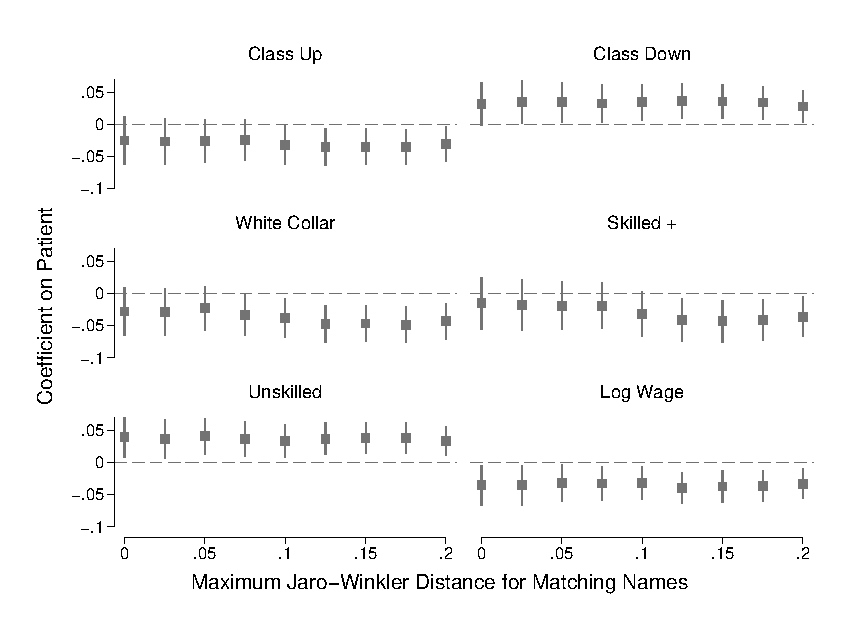
\includegraphics[width=1.0\linewidth]{../output/01_paper/figure_01a.eps}
    \caption{Occupational outcomes}
    \label{fig:jw-robust-occupational}
\end{subfigure}
\begin{subfigure}{0.46\textwidth}
    \centering
    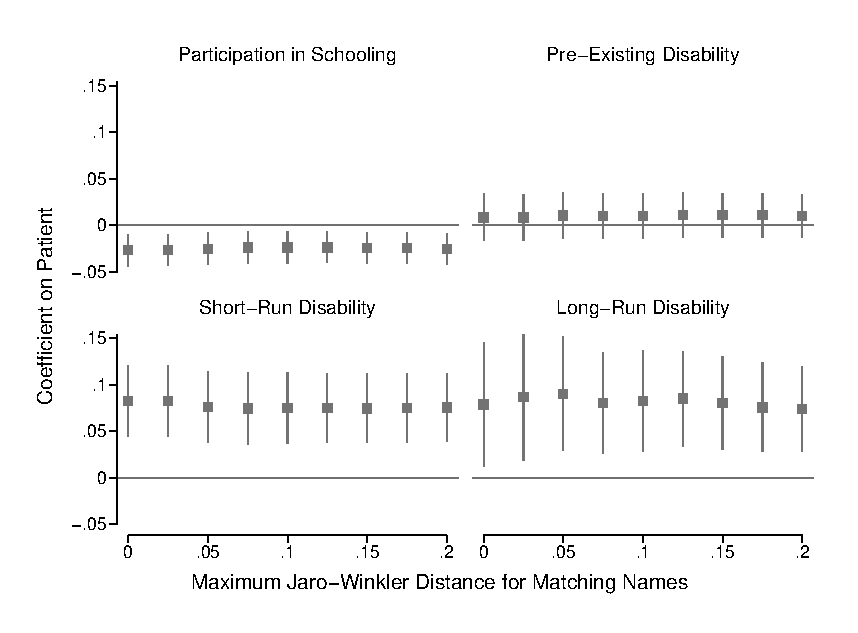
\includegraphics[width=1.0\linewidth]{../output/01_paper/figure_01b.eps}
    \caption{Mechanisms}
    \label{fig:jw-robust-mechanisms}
\end{subfigure}
\Fnote{This figure presents estimated coefficients on the patient indicator variable and 95-percent confidence intervals from separate regressions in which we decrease the Jaro-Winkler distance threshold for inclusion in the sample, moving from the right to the left side of the figures. The long-run occupational outcomes are shown in Figure~\ref{fig:jw-robust-occupational} and the mechanisms are shown in Figure~\ref{fig:jw-robust-mechanisms}. The left side ($x = 0$) of each figure corresponds to the restriction that names must match exactly across censuses and hospital-to-census linkages, while the right side ($x = 0.2$) corresponds to the main sample where Jaro-Winkler distances of up to 0.2 are tolerated. See Tables~\ref{tab:TabLR_Occup_Main} and \ref{tab:Tab_Mechanisms} for a description of the empirical specifications in Figures~\ref{fig:jw-robust-occupational} and \ref{fig:jw-robust-mechanisms}, respectively. The disability outcomes are multiplied by 10 for ease of visualization. With the exception of the long-run disability outcome, which is based on a sample of linked males only, the disability and participation in schooling outcomes use samples that are pooled across genders. Standard errors are clustered by childhood household. The corresponding figure with the single marital status outcome is shown in Online Appendix Figure~\ref{fig:robust-single-marital-status}.}
\label{fig:jw-robust}
\end{figure}
\end{landscape}

% Figure 2
\begin{sidewaysfigure}[!ht]
\caption[Robustness to changing similar names threshold (JW = 0.1)]{Robustness to changing similar names threshold (JW = 0.1)}
\centering
\begin{subfigure}{0.46\textwidth}
	\centering
	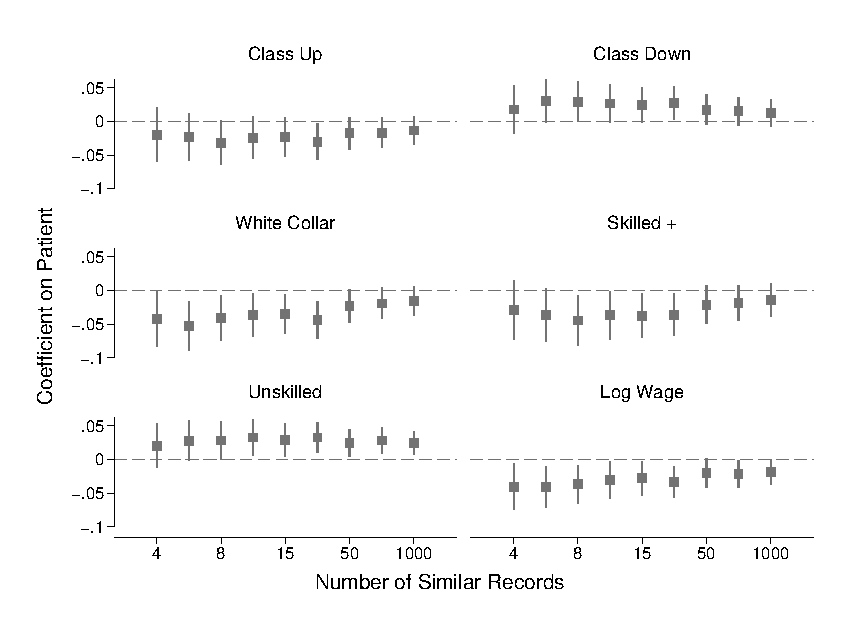
\includegraphics[width=1.0\textwidth]{../output/01_paper/figure_02a.eps}
	\caption{Occupational outcomes}
	\label{fig:sim-10-occupational}
\end{subfigure}
\begin{subfigure}{0.46\textwidth}
	\centering
	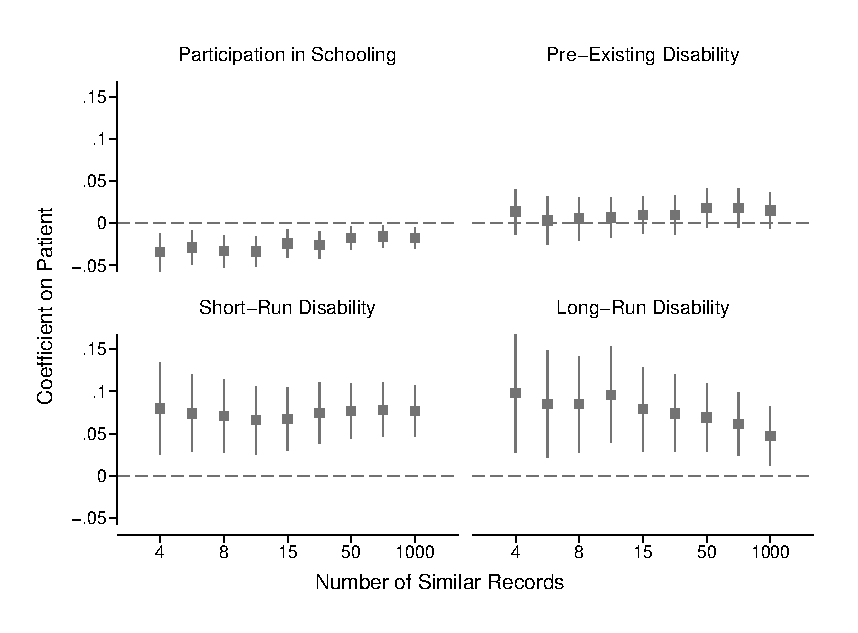
\includegraphics[width=1.0\textwidth]{../output/01_paper/figure_02b.eps}
	\caption{Mechanisms}
	\label{fig:sim-10-mechanisms}
\end{subfigure}
\Fnote{This figure presents estimated coefficients on the patient indicator variable and 95-percent confidence intervals from separate regressions in which we vary the number of records permitted to have similar names that are within one year of birth for a uniquely matched record to be included in the sample. Moving from the left to the right side of the figures, we increase the number of similar records allowed. Similar names are defined as differing in Jaro-Winkler scores by less than 0.1 for the first and last names compared to the name of the matched individual. The long-run occupational outcomes are shown in Figure~\ref{fig:sim-10-occupational} and the mechanisms are shown in Figure~\ref{fig:sim-10-mechanisms}. The main specification corresponds to the estimates with 20 similar names and a Jaro-Winkler threshold of 0.1 for a name to be similar to the matched record. See Tables~\ref{tab:TabLR_Occup_Main} and \ref{tab:Tab_Mechanisms} for a description of the empirical specifications in Figures~\ref{fig:sim-10-occupational} and \ref{fig:sim-10-mechanisms}, respectively. The disability outcomes are multiplied by 10 for ease of visualization. With the exception of the long-run disability outcome, which is based on a sample of linked males only, the disability and participation in schooling outcomes use samples that are pooled across genders. Standard errors are clustered by childhood household. The corresponding figure with the single marital status outcome is shown in Online Appendix Figure~\ref{fig:robust-single-marital-status}.}
\label{fig:sim-names}
\end{sidewaysfigure}

% Figure 3
\begin{sidewaysfigure}[!ht]
\caption[Robustness to changing age-gap threshold for linking]{Robustness to changing age-gap threshold for linking}
\centering
\begin{subfigure}{0.46\textwidth}
    \centering
    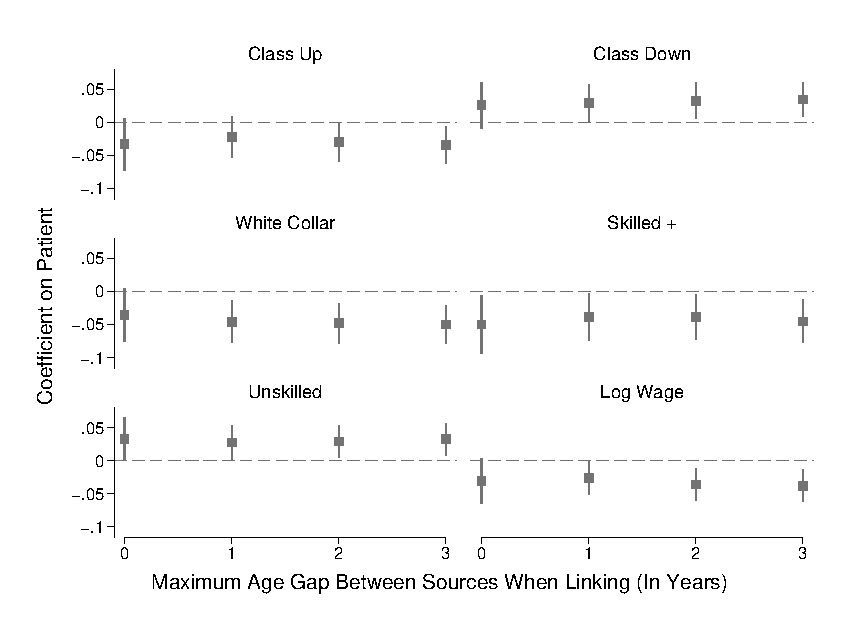
\includegraphics[width=1.0\linewidth]{../output/01_paper/figure_03a.eps}
    \caption{Occupational outcomes}
    \label{fig:age-gap-robust-occupational}
\end{subfigure}
\begin{subfigure}{0.46\textwidth}
    \centering
    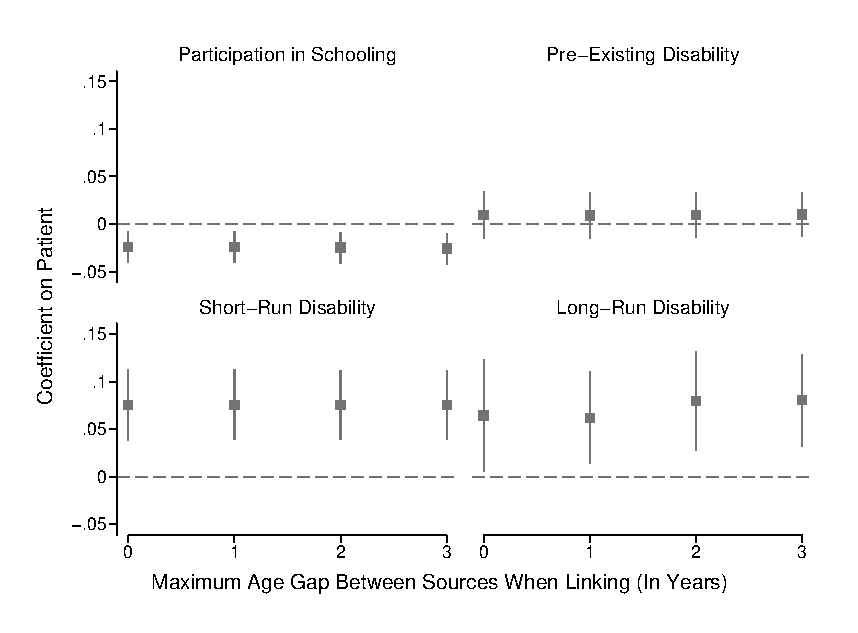
\includegraphics[width=1.0\linewidth]{../output/01_paper/figure_03b.eps}
    \caption{Mechanisms}
    \label{fig:age-gap-robust-mechanisms}
\end{subfigure}
\Fnote{This figure presents estimated coefficients on the patient indicator variable and 95-percent confidence intervals from separate regressions in which we decrease the threshold for differences in reported ages when linking between hospital and census records or between multiple censuses, moving from the right to the left side of the figures. The long-run occupational outcomes are shown in Figure~\ref{fig:age-gap-robust-occupational} and the mechanisms are shown in Figure~\ref{fig:age-gap-robust-mechanisms}. The left side $(x = 0)$ of each figure corresponds to the restriction that ages must match exactly across censuses and hospital-to-census linkages, while the right side $(x = 3)$ corresponds to the main sample where differences in ages of up to 3 years are tolerated. See Tables~\ref{tab:TabLR_Occup_Main} and \ref{tab:Tab_Mechanisms} for a description of the empirical specifications in Figures~\ref{fig:age-gap-robust-occupational} and \ref{fig:age-gap-robust-mechanisms}, respectively. The disability outcomes are multiplied by 10 for ease of visualization. With the exception of the long-run disability outcome, which is based on a sample of linked males only, the disability and participation in schooling outcomes use samples that are pooled across genders. Standard errors are clustered by childhood household. The corresponding figure with the single marital status outcome is shown in Online Appendix Figure~\ref{fig:robust-single-marital-status}.}
\label{fig:age-gap-robust}
\end{sidewaysfigure}

%------------------------------------------%
%                Online Appendix
%------------------------------------------%
\appendix

\renewcommand{\thesection}{\Alph{section}}
\renewcommand{\thesubsection}{\thesection.\arabic{subsection}}
\renewcommand{\thesubsubsection}{\thesubsection.\arabic{subsubsection}}

\newpage
\FloatBarrier
%\newgeometry{left=1in,top=1in,bottom=1in,right=1in}
\setcounter{page}{1}
\setcounter{footnote}{0}

\section*{For Online Publication: Online Appendix\label{sec:online-appendix}}
\addcontentsline{toc}{section}{Online Appendix}

\onehalfspacing

\noindent This document contains supplementary materials for the paper "Lifetime and intergenerational consequences of poor childhood health" by Krzysztof Karbownik and Anthony Wray published in the Journal of Human Resources. 

\section{Data linking procedure\label{sec:linking-procedure}}

In this section we describe the linking algorithms used to match inpatient admission records to census records and to match individuals across censuses. We explain the census-to-census linkage in detail as it is the most basic procedure and it is the basis for the hospital-to-census linkage with some modifications. The description applies to the linkage of male patients and their siblings for the analysis of long-run occupational outcomes. Where applicable, we indicate how the linkage procedure differs for the analysis of mechanisms (participation in schooling and disability) for which only a hospital-to-census linkage is required. We describe the procedure for linking men and women to study effects on the probability of being enumerated as a single adult in Online Appendix Section~\ref{subsubsec:link-marital-status}, and the procedure for linking fathers in Online Appendix Section~\ref{sec:linking-fathers}.

\subsection[Census-to-census linkages]{Census-to-census linkages\label{sec:linking-census-census}}

We use the complete count data for the Censuses of England from the I-CeM project to create five linked samples: 1881 to 1901, 1881 to 1911, 1891 to 1901, 1891 to 1911, and 1901 to 1911 \citep{SchurerHiggs2020,SchurerHiggs2022}.\footnote{We also link the 1881 and 1891 censuses but only use this sample in the auxiliary analysis of fathers described in Online Appendix Section~\ref{sec:linking-fathers}.} In each case, we start with all males aged 0 to 21 in the base year census. Census-to-census linkages are based on time-invariant characteristics such as first name, surname, birth year, and county of birth.\footnote{We choose not to match on birth parish during the initial step given that the variable is a non-standardized text string and parish boundaries changed significantly over the time period of study \citep{SchurerDay2019}.} We begin by separating given names into first and middle names, and then standardize diminutives and common nicknames of first names to their proper equivalents. We follow the procedure in \cite{Parman2015-EEH} and construct the Phonex codes for the first and last names in each data set, which enables us to allow for differences in the spelling of phonetically similar names across data sets that might arise from factors such as typographical errors.\footnote{See \cite{DahisNixQian2020} and the supplemental materials to \cite{Parman2015-EEH} for discussions of the Phonex algorithm.} Prior to the implementation of the matching algorithm, we perform a ``blocking'' step in which the two data sets are joined using four blocking variables: the Phonex code of the first and last names, age in years when enumerated in the later census, and county of birth \citep{Christen2012}. 

The linkage procedure draws on elements of the methods pioneered by \cite{Ferrie1996} and utilized by \cite{ABE2012}, modifications developed by \cite{Feigenbaum2016} and \cite{MillStein2016}, and recommendations made by \cite{BaileyColeHendersonMassey2020}.\footnote{While the linking methods used in this paper are not exact replications of traditional methods, the approach of incorporating features from different methods is validated by the findings of \cite{BaileyColeHendersonMassey2020} that using a combination of samples generated with the \cite{Ferrie1996} and \cite{Feigenbaum2016} methods results in a much lower Type I error rate.} It proceeds as follows: 

\begin{enumerate}
	\item Re-code all births in the counties of Kent, Middlesex, and Surrey as births in ``London'' to account for changes in county boundaries over time and the fact that many people simply report their place of birth as ``London'' in the 1911 census.
	\item Drop all pairs of linked observations that do not have matching Phonex codes or county of birth, while allowing for discrepancies in the reported age of up to 3 years.
	\item Compute the Jaro-Winkler score between the first names and last names in each pair of observations. Discard all pairs with a Jaro-Winkler score less than 0.75 for either the first or last name.\footnote{Economic historians have preferred the Jaro-Winkler score as a string distance measure for linking names across censuses because it places greater weight on characters that match at the beginning of a string \citep{Feigenbaum2016,MillStein2016}. Jaro-Winkler scores range from 0 to 1, where a score of 0 indicates no common letters, while a score of 1 indicates a perfect match. For more details on the Jaro-Winkler method, and other string comparison algorithms, see \cite{Christen2012}.} For first names, we use both the original string and the edited string, and take the highest Jaro-Winkler score among all possible comparisons of first name strings between the two censuses. 
	\item For each record in the earlier census, determine the maximum Jaro-Winkler score averaged over the first and last names, and the minimum discrepancy in age among all records identified in Step 2. Count the number of records in the later census with a Jaro-Winkler score $(J_{s})$ satisfying $(1+0.1)\,J{}_{s}\geq\overline{J}$, where $\bar{J}$ is the Jaro-Winkler score of the best match, and having a reported age within one year of the closest match. 
	\item Prioritize linked observations that match on birth parish.
	\item Drop all pairs of linked observations with a discrepancy in reported age greater than the minimum discrepancy across all later-year census records matched to an earlier-year census record.
	\item Drop any remaining pairs of linked records with a Jaro-Winkler score $(J_{s})$ satisfying $(1+0.1)\,J{}_{s}<\overline{J}$, where $\bar{J}$ is the Jaro-Winkler score of the best match. In other words, we consider a record uniquely matched on name-age combinations if it is sufficiently ``better'' than the next closest match.
	\item Keep all pairs of linked records with a Jaro-Winkler score greater than 0.80 for both the first and last names, that satisfy the following conditions: each earlier-year census has a unique match in the later-year census, and each later-year census record has a unique match in the earlier-year. We exclude records that have unique name-age combinations if the second best match is sufficiently similar.
\end{enumerate}

We present linkage rates separately for all census-to-census linkages in Online Appendix Table~\ref{tab:TabM_ICEM_Census_Match_Rates}. The share of unique matches ranges from 51 to 64 percent across the set of census pairs, with higher match rates for censuses that are closer together, especially those that are only 10 years apart. The census-to-census linkage rates typically found in the literature using complete-count U.S. census data are somewhat lower. This difference can be explained in part by applications with longer windows of time between censuses, typically 30 to 40 years, where sample attrition is of greater concern. Furthermore, the U.S. censuses have less precise information on birth place, at the state level instead of county or parish, which reduces the likelihood of finding unique matches. 

\subsection[Hospital-to-census linkage]{Hospital-to-census linkage\label{sec:linking-hosp-census}}

The procedure for linking inpatient hospital admission records to population censuses follows the steps outlined above for census-to-census linkages with a few important modifications. First, we do not observe place of birth in the hospital records and thus do not use it as a linking variable. Second, we do not require that each census record is linked to a unique admission record, given that we do not observe a patient identifier and some patients may be admitted multiple times. Instead, we treat multiple admission records that match to the same census records as belonging to the same person.

We link each hospital admission record to the 1881, 1891, and 1901 censuses provided that the admission occurred within 10 years of the census enumeration date. We do so for both boys and girls. We use information on the age in years on the day of the hospital admission to determine the age in years on the days of census enumeration. As with the census-to-census linkages, we require the age to differ by no more than 3 years between sources. In the absence of information on place of birth, we prioritize linkages of records that match on county of residence, but we do not require either district or county of residence to match since individuals moved often, even in short time windows between hospital admission and census enumeration. We discuss the overall linkage rates from hospital records to censuses in Section~\ref{subsec:census-data}.  

\subsection[Multiple linkages to a sample of unique individuals]{Multiple linkages to a sample of unique individuals\label{sec:resolve-unique-match}}

In order to execute our empirical strategy we must perform three separate linkages: 
\begin{enumerate}
	\item Patients, from hospital admission records to childhood census records
	\item Patients, from childhood census record to census record during adulthood
	\item Siblings, from childhood census record to census record during adulthood
\end{enumerate}
As a substantial portion of the starting sample is lost through multiple linkages, we must compensate by pooling together multiple hospital-to-census and census-to-census linkages. This section describes the procedure used to identify which records belong to the same individual, and which linked records to use in the analysis for a given individual. 

As described in Section~\ref{sec:hospitaldata}, the hospital admission records do not include a unique patient identifier. We start by assuming that separate admissions belong to the same person if the surname, first name, middle name, implied birth year, and registration district of residence all match across a set of admission records. We use the grouping of records based on these variables as a proxy patient identifier.

Among those patients linked to census records during childhood, we update the unique identifiers based on the census linkages. In a small number of cases, admissions of patients with different proxy identifiers are linked to the same census record in either 1881, 1891, or 1901, and we consider them to be the same individual. When we conduct the second linkage to census records during adulthood, we further consolidate the proxy identifiers. For example, if one admission record is linked to the 1881 census, and another record is linked to the 1891 census, and both census records are linked to the same individual in either the 1901 or 1911 census, then we consider the two admission records to belong to the same patient. As illustrated in Table~\ref{tab:TabM_HOSP_ICEM_Aggregate_Males}, many patients are linked to more than one census, with hospital-to-census linkage rates ranging from 25 to 28 percent for each of the 1881 through 1901 censuses, and 34 percent of patients matched to any census. 

To select the patient and census record pair to use in the analysis of long-run occupational outcomes, we implement an algorithm which prioritizes linkages according to the following criteria: 

\begin{enumerate}
    \item Choose the census closest to the admission year.
    \item Select the census record with the smallest deviation in age between the hospital admission record and the childhood census.
    \item Choose the childhood census record linked to the latest census year during adulthood (1901 or 1911).
    \item Choose the earliest childhood census record (1881, 1891 or 1901). 
\end{enumerate}
Upon completion of these steps, we update the proxy patient identifiers and repeat the procedure once more. The samples used in the main analysis of occupational outcomes and disability in adulthood are formed by pooling together individuals from the three childhood census years (1881, 1891 or 1901) who were linked to either of the adulthood census years (1901 or 1911).

\subsection{Patient-sibling comparisons\label{subsubsec:pat-sib-comp}}

When linking the male siblings of male hospital patients across census years, we attempt to match all siblings within 8 years of age of the patient. In the main regression analysis, we impose some restrictions to limit the sample to comparisons of one patient and one sibling per household:
\begin{enumerate}
    \item Drop households with multiple patients.
    \item Among successfully matched male siblings, keep the sibling who is closest in age to the hospital patient. In the cases where we link both an older and younger sibling with the same age gap in comparison to the hospital patient, we choose the older sibling if the patient's unique identifier in the I-CeM complete count files is an even number and the younger sibling if it is an odd number, in order to avoid biasing the sibling fixed effects comparisons to either younger or older siblings.
\end{enumerate}

\subsection{Linking to long-run marital status: Likelihood of enumeration as a single adult \label{subsubsec:link-marital-status}}

Here we describe the process of generating the samples used to study the effects on the likelihood of being enumerated as a single adult for men and women that are presented in Table~\ref{tab:TabLR_Single_Marital_Status}. The starting point for the analysis of women in column 1 is the sample of girls admitted to a hospital as children and linked to 1881, 1891, or 1901 Censuses of England, along with their sisters who were enumerated in the same household, which we discussed above in Online Appendix Section~\ref{sec:linking-hosp-census}. In comparison to the main analysis, we impose a further restriction that individuals must be no older than age 15 when enumerated in the childhood census. Online Appendix Figure~\ref{fig:Fig_MarriedByAge} shows that only a trivial number of girls below the age of 16 are married, based on the 1911 complete-count census data, and thus this restriction ensures that our sample of patients and their siblings is not biased by selection into marriage. As with the main analysis we match patients to multiple censuses and select a single linked pair of records for each patient based on the following steps:
\begin{enumerate}
    \item Choose the census closest to the admission year.
    \item Select the census record with the smallest deviation in age between the hospital admission record and the childhood census.
    \item Choose the earliest census data (1881 or 1891).
\end{enumerate}
\noindent We restrict the sample to siblings within 5 years of age of the patient. We then attempt to link patients and siblings to censuses 10, 20, or 30 years later, restricting to women who are single and at least 18 years old in the later census. We ensure that linked women are in fact single by excluding individuals who report ever being married. The outcome variable in the regressions is an indicator for a successful linkage to a single women in at least one of the later censuses. The sample of men in column 2 is constructed in identical fashion. In column 3 we restrict the sample to men who are successfully linked to one of the later censuses irrespective of their marital status.

\subsection{Linked samples for analysis of participation in schooling\label{sec:linking-schooling}}

The algorithm for prioritizing a pair of records within a set of census linkages for a given patient when considering school attendance as an outcome differs slightly in comparison to the case of long-run outcomes and proceeds as follows:

\begin{enumerate}
    \item Choose the census closest to the admission year.
    \item Select the census record with the smallest deviation in age between the hospital admission record and the childhood census.
    \item Prioritize matches to census records of school-aged individuals at the time of enumeration.
    \item Choose the most recent census data (1881 or 1891).
\end{enumerate}

When constructing the linked sample, we match both male and female patients to either the 1881 or the 1891 censuses if they were admitted to the hospital prior to enumeration and were ages 5 to 10 years old at the time of the census. This implies that the estimation sample includes individuals from the 1871 to 1876 birth cohorts linked to the 1881 census and individuals from the 1881 to 1886 birth cohorts linked to the 1891 census. This procedure ensures that we choose the highest quality match for the analysis sample, before we impose additional restrictions so that we observe the individual in the census during the compulsory schooling years and after the hospital admission. 

\subsection{Linked samples for analysis of disability\label{sec:linking-disability}}

For the childhood disability analysis, our sample consists of male and female patients linked from the hospital records to one of the 1881 through 1911 censuses up to 10 years post admission, as well as their siblings located in the same household in the census. In the same manner as in the main occupational analysis, we restrict the sample to patients born between 1870 and 1890 and admitted at ages 0 to 11. We further require that both patients and siblings be 21 years or younger at the time of census enumeration. 

When we turn to disability in adulthood we can only include men in the sample due to name changes at marriage by women. The construction of the long-run sample follows the procedure outlined for the long-run occupational outcomes, but we additionally include individuals with missing occupational outcomes. In a separate exercise, we examine whether hospitalization is associated with within-household differences in the likelihood of disability prior to admission. In this case, the sample construction is identical to the childhood disability sample, with the exception that patients are linked from the hospital records to a census up to 10 years before admission.

\subsection[Linked sample of fathers]{Linked sample of fathers\label{sec:linking-fathers}}

Thus far, we have described methods for linking population censuses over time and to hospital admission records, which we use to generate our main analysis samples. In an auxiliary analysis discussed in Section~\ref{subsec:Mechanisms} and reported in Online Appendix Figure~\ref{fig:intragen-fathers}, we also make use of a sample of fathers linked between adjacent censuses. The starting points for the linked sample of fathers are the samples of children age 0 to 21 linked from the 1881 to 1891 and 1891 to 1901 censuses. We append to these samples pairs of census records that are linked to the same hospital patients. We require children to be enumerated in the same household as their father and for their father to report an occupation in both censuses.

Starting from this baseline sample, the minimum criteria for a father to be considered linked are a difference in age of no more than 3 years and a Jaro-Winkler distance of no more than 0.2 for first names (with an exception for initial-to-full name matches). We then drop ``weak'' links with a Jaro-Winkler distance for first names greater than 0.1, no initial match, an age difference greater than 1 year, and non-matching place of birth. A birth place is considered matched if either the county or parish of birth matches (allowing for one string to be contained in the other). Among remaining cases in census A (baseline) with more than one potential match in census B (target), we sequentially prioritize links with the following criteria:
\begin{enumerate}
    \item Same county of birth
    \item Same parish of birth
    \item Same occupational string (allowing for one string to be contained in the other)
    \item Closest match on age
\end{enumerate}
\noindent We then repeat the above steps for records in census B with more than one potential link to census A. We keep individuals whose fathers are uniquely matched in both directions. At this stage, the sample includes individuals whose father is uniquely linked from one census to the next. The remaining step considers cases in which there is more than one potential link for a set of siblings. Again, we repeat the above four steps to prioritize links and keep fathers who are uniquely matched in both directions. Our analysis excludes parishes with no hospital patients and drops households in which a patient is admitted to a hospital either before or after the linking window, but not within it.

\section{Transition matrices and the interpretation of absolute and relative mobility measures \label{sec:transition-matrix-mobility}}

\subsection{Occupational transition matrix}\label{subsec:matrix}

 Online Appendix Table~\ref{tab:TabD_PatSib_Mobility_Matrix} presents occupational transition matrices for households in our main estimation sample. Each column represents the occupational ranks of the fathers (white collar, skilled, semi-skilled, and unskilled) and each row represents the ranks of patients (panel A), control siblings (panel B), patients and siblings combined (panel C), and a synthetic population of linked fathers and sons in England (panel D). The synthetic population is constructed by sampling from five linked samples (1881-1901, 1891-1901, 1881-1911, 1891-1911, and 1901-1911) with sampling probabilities corresponding to the shares of each linked sample in the main estimation sample. Within each panel, a cell reports the percentage of sons in a given rank conditional on father's occupational rank, and thus the percentages sum to 100 across the four rows in each column. The diagonal elements represent cases in which the father and son are observed to have the same occupational rank, while elements above the diagonal are cases of ``upward'' mobility in which sons have a higher rank than their father, and elements below the diagonal represent ``downward'' mobility. For example, among patients in panel A, 45.8 percent of children whose father worked in a white collar occupation also worked in a white collar occupation themselves, but 11.0 percent ended up in unskilled occupations despite their father's high occupational rank. For control siblings in panel B, the corresponding figures are 49.7 percent and 9.0 percent, respectively, suggesting that poor childhood health might be linked, at least descriptively, to downward occupational mobility. Panels C and D provide descriptive measures of mobility in our main estimation sample and a benchmark population, respectively, which we use to assess the magnitude of our main results in Section~\ref{sec:MainResults}.

\subsection{Interpretation of absolute and relative mobility measures}\label{subsec:mobility_interpretation}

Here, we provide an illustrative example to highlight how the sibling fixed effects estimator for the effect of childhood health deficiency will differ in specifications with the relative mobility outcomes compared to those with the absolute occupational outcomes. Recall that we introduced these outcomes in Section~\ref{subsec:hisclass} and highlighted the differences in their respective interpretations as the former capture changes in status relative to one's father across the occupational distribution, whereas the latter measure the likelihood of attaining a rank at a specific part of the occupational distribution. Now, consider two households in which the father is observed in an unskilled occupation. In the first household, the healthy sibling is observed in a skilled occupation, while the hospitalized patient enters an unskilled occupation similar to his father. In the second household, the hospitalized patient ends up in a semi-skilled occupation while the healthy sibling enters a white collar occupation. 

If we consider the first household, the relative outcome of upward mobility will differ between patient and sibling, since only the sibling moves up in status relative to his father, whereas in the second household there is no difference in relative mobility between patient and sibling, since both improve in occupational rank compared to their father. Importantly, the coefficients on upward and downward mobility are not necessarily of equal magnitude and of opposite sign. Households in which one sibling moves up in status and the other moves down relative to the father will have differences between patient and sibling in both the upward and downward mobility outcomes. Yet, a household in which one sibling moves up and and the other stays in the same occupation as their father will have positive upward but zero downward mobility, while a household with one sibling moving down and the other staying in the same occupation as their father will have positive downward but zero upward mobility. The latter case highlights a limitation of the relative mobility outcome in that it does not distinguish between differences in the degree of upward mobility, i.e. rising by two social ranks is better than rising by one rank. Nonetheless, we include the relative mobility measures since the interpretation of these outcomes is comparable to the analysis of transition matrices that has been explored extensively in the occupational mobility literature \citep{LongFerrie2013, Feigenbaum2018, Perez2019}. 

Regardless, we also examine absolute mobility outcomes such as an indicator for white collar occupational status. For the second household in the example, there is a difference in absolute outcomes between patient and sibling, given that ending up in the middle of the occupational distribution is worse than rising to the top. However, in the first household, there is no difference in white collar status between patient and sibling, as neither attains white collar status. In the final empirical sample, 25 to 28 percent of households have variation in the mobility measures while 20 to 39 percent have variation in the own rank outcomes. An indicator for households with patient-sibling pairs that have variation in outcomes is uncorrelated with potentially confounding explanatory variables such as father's age categories, sibship size, characteristics of the patient's linkage to the census, and whether the household is located in the hospital's catchment area. As the example illustrates, in specifications with a relative mobility outcome, a different set of households contribute non-zero differences to the sibling fixed effects estimator compared to specifications with the absolute occupation outcomes. Thus, the estimates will differ and capture complementary but distinct measures of occupational success.

\section{Health Deficiency Index\label{sec:health-deficiency-index}}
In this section we describe the procedure used to construct the health deficiency index introduced in Section~\ref{sec:hospitaldata}. We start with the set of all admissions of male and female patients from the 1870 to 1902 birth cohorts who were admitted to a hospital between 1870 and 1902. Note that the estimation sample includes patients from the 1891 to 1902 birth cohorts who are excluded from the main analysis since they are too young to have occupational outcomes in the available census years. We clean the cause-of-admission text strings and categorize the information into one of seven groups:

\begin{enumerate}
	\singlespacing
	\item Disease or medical conditions
	\item Symptoms
	\item Conditions requiring surgery
	\item External factors (e.g. poisoning or collisions)
	\item Foreign objects
	\item Descriptors of severity
	\item Body parts
\end{enumerate}

\noindent If an individual's admission record $n$ reports one or more diseases or medical conditions, we take the set of these diagnoses as the cause of admission. If not, we go sequential down the list, adding information until we have assigned a primary diagnosis to all possible individuals. 

For each diagnosis, we compute its frequency and observed inpatient mortality rate by gender $g$. Then, for individuals with multiple diagnoses, we choose the diagnosis with the highest mortality rate. We break ties by choosing the most frequently occurring diagnosis. This procedure leaves us with a single primary diagnosis per admission record, which we denote $C_{n}^g$.

Next, we estimate the following linear probability model separately by gender and save the residuals:

\begin{equation}
    P(\textit{Death in hospital})_{nhay}^g = \alpha + \theta_{h} + \delta_{a} + \gamma_{y} + \epsilon_{nhay}^g\label{eq:hospdeath}
\end{equation}

\noindent where $n^g$ indexes individual in-patient admissions for gender $g$, $h$ indexes hospitals, $a$ indexes age in years at admissions, and $y$ indexes the year of admission. The dependent variable is an indicator that takes the value of one when a patient dies in the hospital. We include hospital ($\theta$), age at admission ($\delta$), and year of admission ($\gamma$) fixed effects. We save the residuals $\widehat{\epsilon_{nhay}^g}$ from the regression to use as an input in the next step of computing the health deficiency index. 

The estimation excludes observations with no diagnosis and diagnoses with at least 25 observations for which there is no variation in observed inpatient mortality.\footnote{We take 25 observations as the threshold at which we are confident that the cause of admission is certain not to result in a death in the hospital. There are no causes of admission with more than 25 observations for which all patients die in the hospital. Results are similar when we use thresholds of 10 or 50 observations.} Next, we assign patients the average residual mortality risk for their primary diagnosis as a proxy for childhood health. For each diagnosis $d_{j}^g$ of gender $g$, we compute the following:

\[
    H_{j}^g=\frac{\sum_{n=1}^{N^g}\left(I(d_{j}^g = C_{n}^g)\cdot\widehat{\epsilon_{nhay}^g}\right)}{\sum_{n=1}^{N^g}\left(I(d_{j}^g = C_{n}^g)\right)}
\]

\noindent which is the average unexplained mortality risk across all admissions of gender $g$ with primary diagnosis equal to $d_{j}^g$. Finally, we compute the health deficiency index by the following steps:

\begin{enumerate}
	\item Among diagnoses for which the average residual mortality $H_{j}^g$ was computed, we construct a max-min standardized score according to:
	\[
		Z_j^g = \frac{H_j^g - min(H_j^g)}{max(H_j^g) - min(H_j^g)}
	\]
	\item For diagnoses with at least 25 observations by gender and no observed variation in inpatient mortality, we assign $Z_j^g = 1$ if all patients died in the hospital and $Z_j^g = 0$ if no patients died in the hospital.
\end{enumerate}

\section{Weighting\label{sec:weighting}}

Here, we describe the procedure used to re-weight the data by observable characteristics of all patients in the hospital records. The results are reported in Online Appendix Tables~\ref{tab:TabA_Weight_PatPop} and~\ref{tab:TabA_Weight_PatPop_Single}. Given that the hospital records represent the starting point for our sample construction, we take inpatients at risk of being linked to the census as the baseline population. The at-risk population consists of patients born between 1870 and 1890 and admitted to one of the three hospitals in our sample at ages 0 to 11 between 1870 and 1902. 

We re-weight the data to ensure that the final empirical samples match the proportions in the hospital records based on the following observable characteristics: age at admission, year at admission and place of residence. In specifications involving male and female patients we also re-weight by gender. Our procedure follows \cite{Abramitzky-etal2021} and \cite{Black2020} in that we compute quintile bins for the continuous variables: age at admission (0-1, 2-3, 4-5, 6-8, 9-11) and year of admission (1870-82, 1883-88, 1889-93, 1894-98, 1899-02). Likewise, residential location is measured by the place of residence of a patient at the time of admission. We include indicators for registration districts of London inside and outside a hospital's catchment area, and counties of Greater London (Essex, Kent, Middlesex, and Surrey), with remaining counties as the excluded category. We estimate a probit regression on the population of hospital admissions with the dependent variable equal to one if an individual appears in the final empirical sample. Weights are computed as: $$w=\frac{1}{\widehat{p}}-1$$ where $\widehat{p}$ is the predicted value from the probit regression. Intuitively, we assign higher weight to observations that are less likely to be matched.

%------------------------------------------%
%        Appendix Tables and Figures
%------------------------------------------%

\newpage
\FloatBarrier
\section{Appendix Tables\label{sec:appendix-tables}}
\setcounter{table}{0}\renewcommand{\thetable}{A\arabic{table}}

% Table A1
\begin{table}[ht]\centering
	\begin{adjustbox}{width=.75\textwidth}
	%\setlength{\tabcolsep}{16pt}
	\centering
	\begin{threeparttable}
		\caption{Number of beds and admissions to hospitals in London, 1894
		\label{tab:TabHospAdmitTotal}}
		\vspace{.25ex}
		\textsymbols
		\begin{tabular}{l*{4}{r}}
        \toprule
        \multicolumn{1}{c}{Hospital in 1894} & \multicolumn{1}{c}{\# Beds} & \multicolumn{1}{c}{Inpatients} & \multicolumn{1}{c}{Outpatients} & \multicolumn{1}{c}{Inpatient \%} \\
        \midrule
        &\multicolumn{4}{c}{Panel A: General hospitals} \\
        Barts & 675 & 6,474 & 159,802 & 4.05  \\         
        Guy's & 695 & 6,325 & 57,223 & 11.05 \\ 
        Top-12 General & 4,937 & 52,231 & 688,187 & 7.59 \\   
        \midrule
        Barts share (\%) & 13.7 & 12.4 & 23.2 & \\ 
        Guy's share (\%) & 14.1 & 12.1 & 8.3 & \\
        \midrule
        &\multicolumn{4}{c}{Panel B: Children's hospitals} \\
        GOSH & 178 & 1,801 & 27,334 & 6.59  \\
        Top-6 Children's & 497 & 6,281 & 110,386 & 5.69 \\
        \midrule
        GOSH share (\%) & 35.8 & 28.7 & 24.8 & \\
        \bottomrule
        \addlinespace[.75ex]
        \end{tabular}
		\Fignote{This table displays the number of hospital beds, the number of inpatients, the number of outpatients, and the share of inpatients among outpatients from 1894 for hospitals used in the analysis. The original source does not indicate whether inpatients are included in the outpatient totals. The table also shows the shares for the sample hospitals relative to the twelve largest general and six largest children's hospitals in London (authors' calculations).} \Figsource{\cite{Belgravia1897}.}
	\end{threeparttable}
	\end{adjustbox}
\end{table}

% Table A2
\begin{landscape}
\begin{table}[ht]\centering
	\begin{adjustbox}{width=1.0\textwidth}
	\centering
	\begin{threeparttable}
		\caption{Common causes of admission in hospital population by gender and in long-run occupational sample \label{tab:top-25-coa}}
		\vspace{.25ex}
		\textsymbols
		\begin{tabular}{l*{4}{r}*{1}{l}*{4}{r}*{1}{l}*{3}{r}}
        \toprule
        \estinput{../output/02_appendix/table_a02.tex}
        \bottomrule
        \addlinespace[.75ex]
        \end{tabular}
		\Fignote{This table lists the 25 most common causes of admission in the populations of hospitalized male and female patients, as well as the sample of males used in the long-run occupational analysis. The hospital populations consist of all admissions by patients born between 1870 and 1902 and admitted at ages 0 to 11 from 1870 to 1902 at GOSH, Barts, or Guy's Hospitals. The causes of admission are tabulated after cleaning the text strings transcribed from the admissions registers. The mortality rate refers to the share of admissions in which a patient died in the hospital. The long-run (LR) sample of males refers to the set of 2,146 hospital admissions reported in column 4 of Table~\ref{tab:TabM_HOSP_ICEM_Aggregate_Males}, which correspond to the 1,849 male patients included in the main analysis in Table~\ref{tab:TabLR_Occup_Main}. The mortality rate is not shown for the long-run sample since it only includes patients who survived until adulthood. In the LR sample, admissions for hip disease and eczema also occurred 21 times.}
	\end{threeparttable}
	\end{adjustbox}
\end{table}
\end{landscape}

% Table A3
\newpage
\begin{table}[!t]\centering
	\begin{adjustbox}{width=0.9\textwidth}
	\centering
	\begin{threeparttable}
		\caption{Common occupational titles by occupational class \label{tab:top-occ-by-class}}
		\estauto{../output/02_appendix/table_a03.tex}{5}{l}
		\Fignote{This table lists the five most common occupations in each of four occupational classes for the final sample of patients and siblings used in the main analysis of long-run occupational outcomes reported in Table~\ref{tab:TabLR_Occup_Main}. Column 1 combines professional, managerial and clerical occupations, which correspond to classes 1 to 5 in the Historical International Social Class Scheme (HISCLASS), into a white collar class. Column 2 subsumes farmers into skilled workers (HISCLASS 6 to 8), column 3 displays semi-skilled workers (HISCLASS 9), and column 4 combines unskilled workers as well as low and unskilled farm workers (HISCLASS 10 to 12). See Section~\ref{subsec:hisclass} for further details on the occupational classification.}
	\end{threeparttable}
	\end{adjustbox}
\end{table}

%Table A4
\newpage
\begin{table}[!ht]\centering
	\begin{adjustbox}{width=1.0\textwidth}
	\centering
	\begin{threeparttable}
		\caption{Intergenerational occupational elasticities \label{tab:TabIGM_PR}}
		\estauto{../output/02_appendix/table_a04.tex}{3}{S[table-format=2.4,table-column-width=30mm]}
		\Fignote{This table presents estimates using data on males aged 0 to 11 linked from the 1881 to the 1911 complete-count census. In each column, the dependent variable is an indicator for the son's occupational status or the son's log occupational wage which are identical to the dependent variables in columns 3, 4, and 6 of Table~\ref{tab:TabLR_Occup_Main}. The treatment variable ``father's status'' varies across the columns and in each case is defined in an equivalent way as the dependent variable but for the father rather than the son. The regressions also control for an indicator for above-median sibship size, match quality dummies, as well as own and father's birth year fixed effects. \Starnote}
	\end{threeparttable}
	\end{adjustbox}
\end{table}

% Table A5
\newpage
\begin{table}[!ht]\centering
	\begin{adjustbox}{width=1.0\textwidth}
	\centering
	\begin{threeparttable}
		\caption{Intergenerational mobility matrix for linked population and estimation samples \label{tab:TabD_PatSib_Mobility_Matrix}}
		\estauto{../output/02_appendix/table_a05.tex}{6}{S[table-format=2.3,table-column-width=20mm]}
		\Fignote{This table presents occupational transition matrices for fathers and sons in the main sample used in Table~\ref{tab:TabLR_Occup_Main} (panels A to C) and in a synthetic population (panel D). Each column represents an occupational class for fathers of individuals in the main sample or synthetic population (from high to low): white collar, skilled, semi-skilled, and unskilled. The stratification of occupational titles into four groups is formed by consolidating the 12 strata of the Historical International Social Class Scheme (HISCLASS) as described in Section~\ref{subsec:hisclass}. In panels A to C, the rows of the matrices represent the occupational class as adult for patients (panel A), siblings (panel B), or patients and siblings (panel C). The set of fathers does not change across the three panels. Within each panel, a cell contains the percentages of sons in each occupational class given the rank of the father. Percentages in a given column may not sum to 100 across its rows due to rounding errors. Panel D represents the transition matrix for a synthetic population constructed by sampling from five linked samples: 1881-1901, 1891-1901, 1881-1911, 1891-1911, and 1901-1911. The sampling probabilities correspond to the share of observations from each linked sample in the main sample. Each linked population consists of males born between 1870 and 1893 who were at least 18 years old in the later census year.}
	\end{threeparttable}
	\end{adjustbox}
\end{table}

% Table A6
\newpage
\begin{sidewaystable}[ht]\centering
	\begin{adjustbox}{width=0.9\textwidth}
	\centering
	\begin{threeparttable}
		\caption{Effects on long-run social outcomes \label{tab:TabA_Social_Outcomes}}
		\estauto{../output/02_appendix/table_a06.tex}{5}{S[table-format=2.4,table-column-width=30mm]}
		\Fignote{This table presents sibling fixed effects estimates of the patient indicator (panel A) and the health deficiency index (panel B) on social outcomes observed at the time of census enumeration during adulthood. In column 1, the dependent variable is the share of individuals who work in unskilled occupations in the parish of residence during adulthood. Unskilled occupations are defined as HISCLASS ranks 10 to 12 and correspond to the outcome in column 5 of Table~\ref{tab:TabLR_Occup_Main}. In column 2, the dependent variable is an indicator for living in the same household as at least one parent. In column 3, it is an indicator for residing in a different county than when enumerated in the census during childhood. In column 4, it is an indicator for having any children. In column 5, it is an indicator for the child participating in schooling (see Section~\ref{subsec:schooling-spec} for details on how the variable is coded). In columns 1 to 4, the sample first restricts attention to individuals in the main empirical sample in Table~\ref{tab:TabLR_Occup_Main}, with further restriction to households in which the outcome variable is not missing for both patient and sibling, but allowing sample individuals and their fathers to have missing occupations. Column 5 also requires both patient and sibling to have a child. See Table~\ref{tab:TabLR_Occup_Main} for a description of the control variables. Standard errors are clustered by childhood household. Percent effects in panel B are computed as $\beta \times \sigma_{HDI}$ scaled by the dependent variable mean, where $\sigma_{HDI} = 0.13$ is the standard deviation of the health deficiency index in the hospital population. \Starnote}
	\end{threeparttable}
	\end{adjustbox}
\end{sidewaystable}

% Table A7
\newpage
\begin{sidewaystable}[ht]\centering
	\begin{adjustbox}{width=0.85\textwidth}
	\centering
	\begin{threeparttable}
		\caption{Heterogeneity by severity and age at admission \label{tab:TabLR-Heterogeneity}}
		\estauto{../output/02_appendix/table_a07.tex}{6}{S[table-format=2.4,table-column-width=20mm]}
		\Fignote{This table presents sibling fixed effects estimates. Panel A displays estimates in which we interact the indicator for hospital patient with indicators for being admitted for conditions with above and below median values of the health deficiency index. Panel B interacts the indicator variable for hospitalization with separate indicators for early- (age 0 to 4) and late-childhood (age 5 to 11) admission, which are coded based on a patient's first observed admission to a hospital. The dependent variables in columns 1 to 6 correspond to those shown in Table~\ref{tab:TabLR_Occup_Main}. See Table~\ref{tab:TabLR_Occup_Main} for a description of the control variables. Standard errors are clustered by childhood household. \Starnote}
	\end{threeparttable}
	\end{adjustbox}
\end{sidewaystable}

%Table A8
\newpage
\begin{table}[t]\centering
	\begin{adjustbox}{width=1.0\textwidth}
	\centering
	\begin{threeparttable}
		\caption{Descriptive statistics for hospital catchment areas\label{tab:TabD-HOSP-catchment-1891}}
		\estauto{../output/02_appendix/table_a08.tex}{4}{S[table-format=1.3,table-column-width=20mm]}
		\Fignote{This table presents descriptive statistics from the 1891 Census of England for the catchment area of each hospital used in the analysis. A hospital's catchment area is defined as the set of registration districts from which the most patients are admitted and which together account for at least 50 percent of total admissions by children age 0 to 11. The Barts Hospital catchment area includes: Holborn, Shoreditch, and Islington. The GOSH catchment area includes: Holborn, Islington, Pancras, Kensington, Marylebone, Shoreditch, and St Giles. The Guy's Hospital catchment area includes: St Olave Southwark and St Saviour Southwark. Results are similar when using the 1881 or 1901 census.}
	\end{threeparttable}
	\end{adjustbox}
\end{table}

%Table A9
\newpage
\begin{table}[ht]\centering
	\begin{adjustbox}{width=.75\textwidth}
	\centering
	\begin{threeparttable}
		\caption{Selection into hospitalization for male patients \label{tab:TabD_HOSP_Selection_Male}}
		\estauto{../output/02_appendix/table_a09.tex}{3}{S[table-format=3.4,table-column-width=20mm]}
		\Fignote{This table presents OLS estimates using a sample that consists of individuals who were ages 0 to 5 and residing in the County of London when enumerated in the 1881, 1891 or 1901 censuses. The dependent variable is an indicator for a unique match to an inpatient hospital admission that occurred up to 10 years after the census enumeration date and when the individual was age 0 to 11 at the time of admission. The regressions also include age-at-enumeration by census-year fixed effects for patients and their fathers. \Starnote}
	\end{threeparttable}
	\end{adjustbox}
\end{table}

% Table A10
\newpage
\begin{sidewaystable}[ht]\centering
	\begin{adjustbox}{width=1.0\textwidth}
	\centering
	\begin{threeparttable}
		\caption{Weighting by characteristics of patient population -- Occupational outcomes and mechanisms \label{tab:TabA_Weight_PatPop}}
		\estauto{../output/02_appendix/table_a10.tex}{10}{S[table-format=3.4,table-column-width=17mm]}
		\Fignote{This table displays sibling fixed effects estimates from regressions that re-weight the data by the following observable characteristics in the hospital records: admission age, admission year, and location of residence in all columns, as well as gender in columns 7 to 9. Re-weighting the data ensures that each linked sample matches the proportions in the population of inpatient hospital admissions. The weighting procedure is described in more detail in Online Appendix~\ref{sec:weighting}. In panel A, the explanatory variable of interest is an indicator for hospital admission, and in panel B, it is the health deficiency index. Columns 1 to 6 present estimates for the outcomes variables shown in Table~\ref{tab:TabLR_Occup_Main}. Columns 7 to 9 display estimates for the schooling and disability mechanisms from the pooled gender samples in Table~\ref{tab:Tab_Mechanisms}, while column 10 reports estimates for long-run disability using the linked sample of boys only. See Tables~\ref{tab:TabLR_Occup_Main} and~\ref{tab:Tab_Mechanisms} for a description of the control variables. Standard errors are clustered by childhood household. Percent effects for log wages (column 6) are calculated using the formula $100 \times exp(\beta) - 1$. Percent effects in panel B are computed as $\beta \times \sigma_{HDI}$ scaled by the dependent variable mean, where $\sigma_{HDI} = 0.13$ is the standard deviation of the health deficiency index in the hospital population. \Starnote}
	\end{threeparttable}
	\end{adjustbox}
\end{sidewaystable}

% Table A11
\newpage
\begin{table}[ht]\centering
	\begin{adjustbox}{width=0.9\textwidth}
	\centering
	\begin{threeparttable}
		\caption{Effects on likelihood of being observed as single for men and women -- Weighting \label{tab:TabA_Weight_PatPop_Single}}
		\estauto{../output/02_appendix/table_a11.tex}{3}{S[table-format=2.4,table-column-width=25mm]}
		\Fignote{This table displays sibling fixed effects estimates from regressions that re-weight the data by the following observable characteristics in the hospital records: admission age, admission year, and location of residence.  Re-weighting the data ensures that each linked sample matches the proportions in the population of inpatient hospital admissions. The weighting procedure is described in more detail in Online Appendix~\ref{sec:weighting}. In panel A, the explanatory variable of interest is an indicator for hospital admission, and in panel B, it is the health deficiency index. The estimates correspond to the outcomes variables and samples used in Table~\ref{tab:TabLR_Single_Marital_Status}. See Table~\ref{tab:TabLR_Single_Marital_Status} for a description of the control variables. Standard errors are clustered by childhood household. Percent effects in panel B are computed as $\beta \times \sigma_{HDI}$ scaled by the dependent variable mean, where $\sigma_{HDI} = 0.13$ is the standard deviation of the health deficiency index in the hospital population. \Starnote}
	\end{threeparttable}
	\end{adjustbox}
\end{table}

% Table A12
\newpage
\begin{table}[ht]\centering
	\begin{adjustbox}{width=1.0\textwidth}
	\centering
	\begin{threeparttable}
		\caption{Long-run outcomes: Robustness to selective mortality \label{tab:TabLR_Robustness_Mortality-HDI}}
		\estauto{../output/02_appendix/table_a12.tex}{6}{S[table-format=2.4,table-column-width=20mm]}
		\Fignote{This table is identical to Table~\ref{tab:TabLR_Robustness_Mortality-Patient} with the exception that the treatment variable is changed from an indicator for hospitalization to the continuous health deficiency index. Standard errors are clustered by childhood household. \Starnote}
	\end{threeparttable}
	\end{adjustbox}
\end{table}

% Table A13
\newpage
\begin{sidewaystable}[ht]\centering
	\begin{adjustbox}{width=0.80\textwidth}
	\centering
	\begin{threeparttable}
		\caption{Long-run outcomes: Robustness to sample selection \label{tab:TabLR_Robustness_SampleSelection-HDI}}
		\estauto{../output/02_appendix/table_a13.tex}{7}{S[table-format=2.4,table-column-width=17mm]}
		\Fignote{This table is identical to Table~\ref{tab:TabLR_Robustness_SampleSelection-Patient} with the exception that the treatment variable is changed from an indicator for hospitalization to the continuous health deficiency index. Standard errors are clustered by childhood household. \Starnote}
	\end{threeparttable}
	\end{adjustbox}
\end{sidewaystable}

% Table A14
\newpage
\begin{table}[ht]\centering
	\begin{adjustbox}{width=1.0\textwidth}
	\centering
	\begin{threeparttable}
		\caption{Long-run outcomes: Robustness to variations in occupational status \label{tab:TabLR_Robustness_Occupations-HDI}}
		\estauto{../output/02_appendix/table_a14.tex}{5}{S[table-format=2.4,table-column-width=20mm]}
		\Fignote{This table is identical to Table~\ref{tab:TabLR_Robustness_Occupations} with the exception that the treatment variable is changed from an indicator for hospitalization to the continuous health deficiency index. Standard errors are clustered by childhood household. \Starnote}
	\end{threeparttable}
	\end{adjustbox}
\end{table}

% Table A15
\newpage
\begin{sidewaystable}[ht]\centering
	\begin{adjustbox}{width=1.0\textwidth}
	\centering
	\begin{threeparttable}
		\caption{Robustness of effects on likelihood of being enumerated as a single adult \label{tab:TabA_Marital_Robustness}}
		\estauto{../output/02_appendix/table_a15.tex}{11}{S[table-format=2.4,table-column-width=20mm]}
		\Fignote{Each cell comes from a separate sibling fixed effects regression. In Panels A to C, the dependent variables and estimation samples are identical to those presented in columns 1 to 3, respectively, of Table~\ref{tab:TabLR_Single_Marital_Status}. Each column represents a separate modification to the main estimation sample. The exercises in columns 1 to 5 are identical to those presented in Table~\ref{tab:TabLR_Robustness_Mortality-Patient}, while the exercises in columns 6 to 11 correspond to Table~\ref{tab:TabLR_Robustness_SampleSelection-Patient}. \Starnote}
	\end{threeparttable}
	\end{adjustbox}
\end{sidewaystable}

%Table A16
\newpage
\begin{sidewaystable}[ht]\centering
	\begin{adjustbox}{width=1.0\textwidth}
	\centering
	\begin{threeparttable}
		\caption{Robustness of participation in schooling outcome \label{tab:TabCH_Scholar_Robust}}
		\estauto{../output/02_appendix/table_a16.tex}{6}{S[table-format=2.4,table-column-width=20mm]}
		\Fignote{Each cell comes from a separate sibling fixed effects regression. Column 1 of panel A reproduces the estimate for the schooling outcome from column 3 of Table~\ref{tab:Tab_Mechanisms}, which is based on a sample of individuals aged 5 to 10 when enumerated in the census. See Table~\ref{tab:Tab_Mechanisms} for a list of variables included in the regressions. See Tables~\ref{tab:TabLR_Robustness_Mortality-Patient} and  \ref{tab:TabLR_Robustness_SampleSelection-Patient} for a description of the sample restrictions in the remaining columns and panels. Standard errors are clustered by childhood household. \Starnote}
	\end{threeparttable}
	\end{adjustbox}
\end{sidewaystable}

%Table A17
\newpage
\begin{sidewaystable}[ht]\centering
	\begin{adjustbox}{width=1.0\textwidth}
	\centering
	\begin{threeparttable}
		\caption{Robustness of pre-existing disability outcome \label{tab:TabCH_PreExisting_Robust}}
		\estauto{../output/02_appendix/table_a17.tex}{6}{S[table-format=2.4,table-column-width=20mm]}
		\Fignote{Each cell comes from a separate sibling fixed effects regression. Column 1 of panel A reproduces the estimate for the pre-existing disability outcome from column 6 of Table~\ref{tab:Tab_Mechanisms}. See Table~\ref{tab:Tab_Mechanisms} for a list of variables included in the regressions. See Tables~\ref{tab:TabLR_Robustness_Mortality-Patient} and  \ref{tab:TabLR_Robustness_SampleSelection-Patient} for a description of the sample restrictions in the remaining columns and panels. Standard errors are clustered by childhood household. \Starnote}
	\end{threeparttable}
	\end{adjustbox}
\end{sidewaystable}

% Table A18
\newpage
\begin{sidewaystable}[ht]\centering
	\begin{adjustbox}{width=1.0\textwidth}
	\centering
	\begin{threeparttable}
		\caption{Robustness of childhood disability outcome \label{tab:TabCH_Disability_Robust}}
		\estauto{../output/02_appendix/table_a18.tex}{6}{S[table-format=2.4,table-column-width=20mm]}
		\Fignote{Each cell comes from a separate sibling fixed effects regression. Column 1 of panel A reproduces the estimate for the childhood disability outcome from column 9 of Table~\ref{tab:Tab_Mechanisms}. See Table~\ref{tab:Tab_Mechanisms} for a list of variables included in the regressions. See Tables~\ref{tab:TabLR_Robustness_Mortality-Patient} and  \ref{tab:TabLR_Robustness_SampleSelection-Patient} for a description of the sample restrictions in the remaining columns and panels. Standard errors are clustered by childhood household. \Starnote}
	\end{threeparttable}
	\end{adjustbox}
\end{sidewaystable}

%Table A19
\newpage
\begin{sidewaystable}[ht]\centering
	\begin{adjustbox}{width=1.0\textwidth}
	\centering
	\begin{threeparttable}
		\caption{Robustness of long-run disability outcomes \label{tab:TabLR_Disability_Robust}}
		\estauto{../output/02_appendix/table_a19.tex}{6}{S[table-format=2.4,table-column-width=20mm]}
		\Fignote{Each cell comes from a separate sibling fixed effects regression. Column 1 of panel A reproduces the estimate for the long-run disability outcome from column 10 of Table~\ref{tab:Tab_Mechanisms}. See Table~\ref{tab:Tab_Mechanisms} for a list of variables included in the regressions. See Tables~\ref{tab:TabLR_Robustness_Mortality-Patient} and  \ref{tab:TabLR_Robustness_SampleSelection-Patient} for a description of the sample restrictions in the remaining columns and panels. Standard errors are clustered by childhood household. \Starnote}
	\end{threeparttable}
	\end{adjustbox}
\end{sidewaystable}

%Table A20
\newpage
\begin{sidewaystable}[ht]\centering
	\begin{adjustbox}{width=1.0\textwidth}
	\centering
	\begin{threeparttable}
		\caption{Sibling-specific determinants of hospitalization \label{tab:TabM_First_Born_Selection}}
		\estauto{../output/02_appendix/table_a20.tex}{8}{S[table-format=2.4,table-column-width=20mm]}
		\Fignote{Columns 1 to 4 present sibling fixed effects estimates with an indicator for hospitalization as the dependent variable, while columns 5 to 8 show OLS estimates with the health deficiency index as the dependent variable when restricting to patients only. Linkages from the 1881, 1891, and 1901 censuses, respectively, to hospital records up to 10 years after the census enumeration date are shown in columns 1 to 3 and 5 to 7. The samples consist of all individuals enumerated at ages 0 to 5 in the County of London in households with at least one patient admitted to the hospital at ages 0 to 11 years old no more than 10 years after the census enumeration date. Columns 4 and 8 pool together the samples in the preceding columns. All regressions include age-at-enumeration by census year fixed effects.  Columns 1 to 4 cluster standard errors by household while columns 5 to 8 report heteroskedasticity robust standard errors. \Starnote}
	\end{threeparttable}
	\end{adjustbox}
\end{sidewaystable}

%Table A21
\newpage
\begin{table}[!ht]\centering
	\begin{adjustbox}{width=0.9\textwidth}
	\centering
	\begin{threeparttable}
		\caption{Patient health deficiency index and likelihood of linkage to census \label{tab:TabM_Health_Deficiency_Index_Match_Rates}}
		\estauto{../output/02_appendix/table_a21.tex}{4}{S[table-format=2.4,table-column-width=20mm]}
		\Fignote{This table presents OLS estimates from specifications in which the dependent variable is an indicator for a unique match from the hospital records to a census. The only explanatory variable is the health deficiency index, the coefficients for which are reported in the table. Columns 1 to 3 present results for linkages from the hospital records to the 1881, 1891, and 1901 censuses, respectively. Column 4 pools together the samples in the preceding columns. The samples consists of all patients admitted to the hospital at ages 0 to 11 years old no more than 10 years prior to the census enumeration date and discharged from the hospital prior to the census enumeration date. \Starnote}
	\end{threeparttable}
	\end{adjustbox}
\end{table}

%Table A22
\newpage
\begin{table}[ht]\centering
	\begin{adjustbox}{width=1.0\textwidth}
	\centering
	\begin{threeparttable}
		\caption{Census-to-census linkage rates
		\label{tab:TabM_ICEM_Census_Match_Rates}}
		\vspace{.25ex}
		\textsymbols
		\begin{tabular}{l*{4}{S[table-format=2.4,table-column-width=20mm]}*{1}{S[table-format=2.4,table-column-width=20mm]}}
        \toprule
        \estinput{../output/02_appendix/table_a22.tex}
        \bottomrule
        \addlinespace[.75ex]
        \end{tabular}
		\Fignote{The table presents census-to-census linkage rates for boys residing in England in the base-year census. See Online Appendix~\ref{sec:linking-census-census} for a description of the linkage procedure.}
	\end{threeparttable}
	\end{adjustbox}
\end{table}

\newpage
\FloatBarrier
\section[Appendix Figures]{Appendix Figures\label{sec:app-figs}}
\setcounter{figure}{0}\renewcommand{\thefigure}{A\arabic{figure}}

% Figure A1
\begin{figure}[!ht]
	\caption[London hospital locations and surviving records]{London hospital locations and surviving records}
	\centering
    \includegraphics[width=1.0\textwidth]{../output/02_appendix/figure_a01.eps}
    %\captionsetup[sub]{skip=15pt}
    \Fnote{A map of central London marking the locations of hospitals in the empirical sample (red squares and triangle), general hospitals (squares symbol), and children's hospitals (triangle symbol). The subset of these hospitals with surviving archival records is marked in green.}
	\label{fig:hospital-records-map}
\end{figure}

% Figure A2
\newpage
\begin{figure}[!ht]
    \caption[Sample inpatient admission register from St. Bartholomew's Hospital]{Sample inpatient admission register from St. Bartholomew's Hospital}
    \centering
    \includegraphics[width=0.90\textwidth]{../output/02_appendix/figure_a02.eps}
    \Fnote{Sample page of an inpatient admission register from November 1890 for St. Bartholomew's Hospital in London. Each page contains the date of admission, the patient's name, age, complaint and address, the name of the ward in which the patient was admitted, the name of the physician or surgeon who treated the patient, and the date of discharge or death. Source: Photograph taken by authors courtesy of Barts Health NHS Trust Archives. Document reference number: SBHB/MR/2/6.}
    \label{fig:sample-hospital-record}
\end{figure}

% Figure A3
\begin{figure}[!ht]
\caption[In-hospital mortality by age at admission]{In-hospital mortality by age at admission}
\centering
\begin{subfigure}{\textwidth}
	\centering
	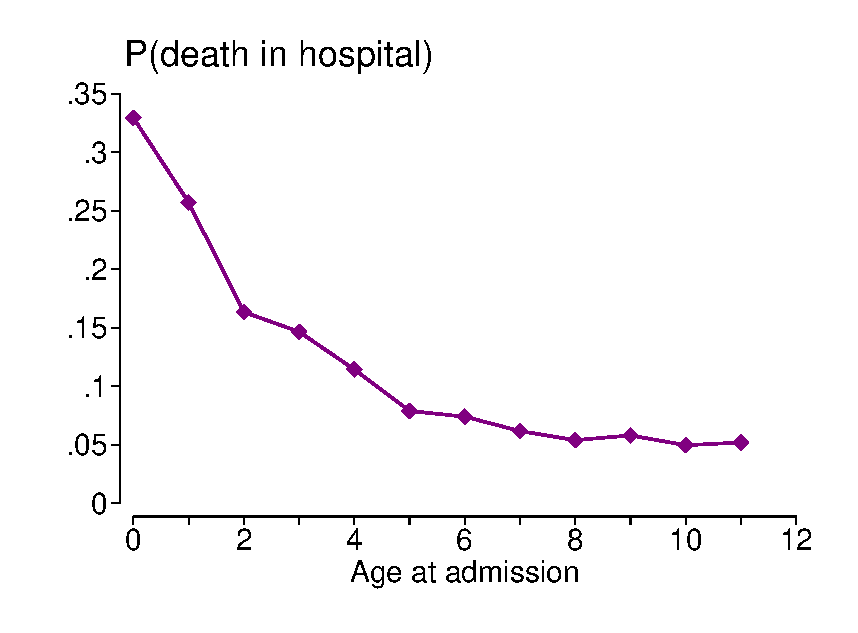
\includegraphics[width=0.65\linewidth]{../output/02_appendix/figure_a03a.eps}
	\caption{Raw data}
	\label{fig:mort-age-raw}
\end{subfigure}
\begin{subfigure}{\textwidth}
	\centering
	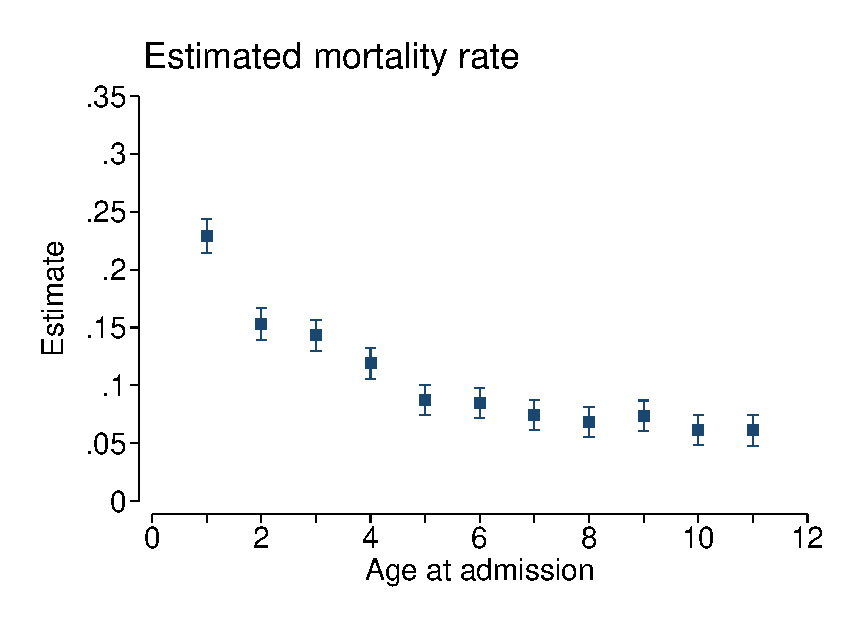
\includegraphics[width=0.65\linewidth]{../output/02_appendix/figure_a03b.eps}
	\caption{Regression adjusted}
	\label{fig:mort-age-reg}
\end{subfigure}
\Fnote{Panel A plots the in-hospital mortality rate by age at admission and Panel B presents regression-adjusted estimates. Panel B plots estimated fixed effects on age at admission (with age 0 as the excluded category) from a linear probability model which also includes admission year, hospital, gender, and number-of-comorbidity fixed effects, as well as indicators for above or below median length of stay, being treated by a doctor, and transferred to another hospital as covariates. The samples include data on all in-patients aged 0 to 11 born between 1870 and 1902, and admitted between 1870 and 1902 to the Hospital for Sick Children at Great Ormond Street, Guy's Hospital, or St. Bartholomew's Hospital, in London.}
\label{fig:hosp-mort-age}
\end{figure}

% Figure A4
\begin{figure}[!ht]
\caption[In-hospital mortality by year of admission]{In-hospital mortality by year of admission}
\centering
\begin{subfigure}{\textwidth}
	\centering
	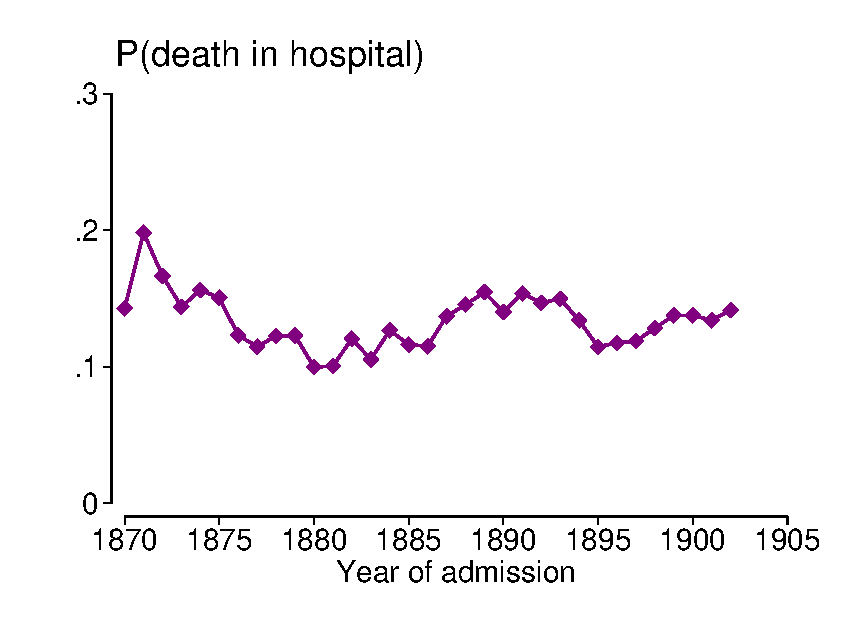
\includegraphics[width=0.65\linewidth]{../output/02_appendix/figure_a04a.eps}
	\caption{Raw data}
	\label{fig:mort-by-yr-raw}
\end{subfigure}
\begin{subfigure}{\textwidth}
	\centering
	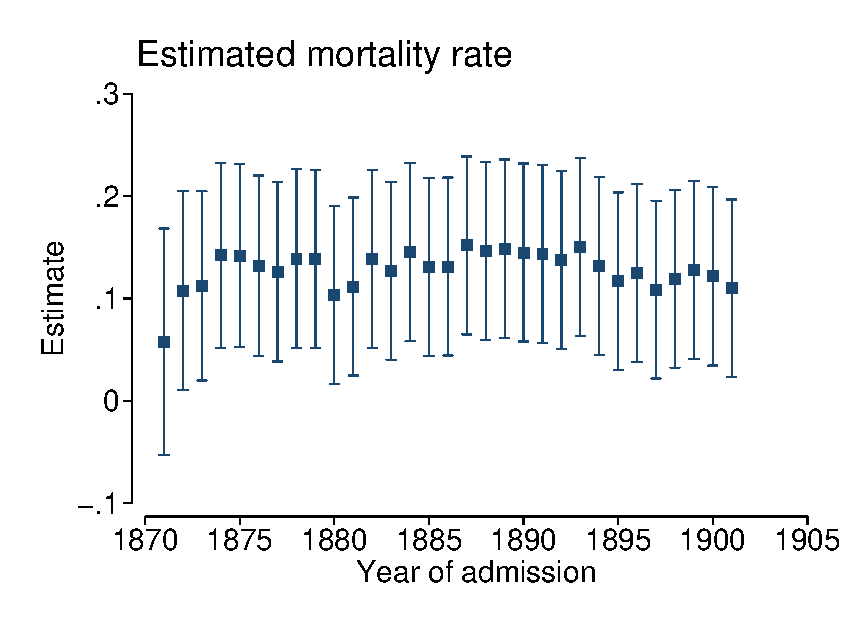
\includegraphics[width=0.65\linewidth]{../output/02_appendix/figure_a04b.eps}
	\caption{Regression adjusted}
	\label{fig:mort-by-yr-reg}
\end{subfigure}
\Fnote{Panel A plots the in-hospital mortality rate by year of admission and Panel B presents regression-adjusted estimates. Panel B plots estimated fixed effects on year of admission (with 1870 as the excluded category) from a linear probability model which also includes admission age, hospital, gender, and number-of-comorbidity fixed effects, as well as indicators for above or below median length of stay, being treated by a doctor, and transferred to another hospital as covariates. The samples include data on all in-patients aged 0 to 11 born between 1870 and 1902, and admitted between 1870 and 1902 to the Hospital for Sick Children at Great Ormond Street, Guy's Hospital, or St. Bartholomew's Hospital, in London.}
\label{fig:hosp-mort-by-yr}
\end{figure}

% Figure A5
\begin{figure}[!ht]
    \caption{Share of children living with a parent in 1881, by age}        	
    \centering
    \includegraphics[width=1.0\textwidth]{../output/02_appendix/figure_a05.eps}
    \Fnote{This figure plots the share of children who were enumerated in the 1881 census in a household in which at least one parent was present. The sample consists of all households in the County of London. Results are similar in the 1891 census. The vertical red line indicates age 11, which is the oldest age at admission of a hospital patient in our data.}
    \label{fig:live-parent-age}
\end{figure}

% Figure A6
\begin{figure}[!ht]
    \caption{Labor force participation and participation in schooling by age in 1881}    
    \centering
    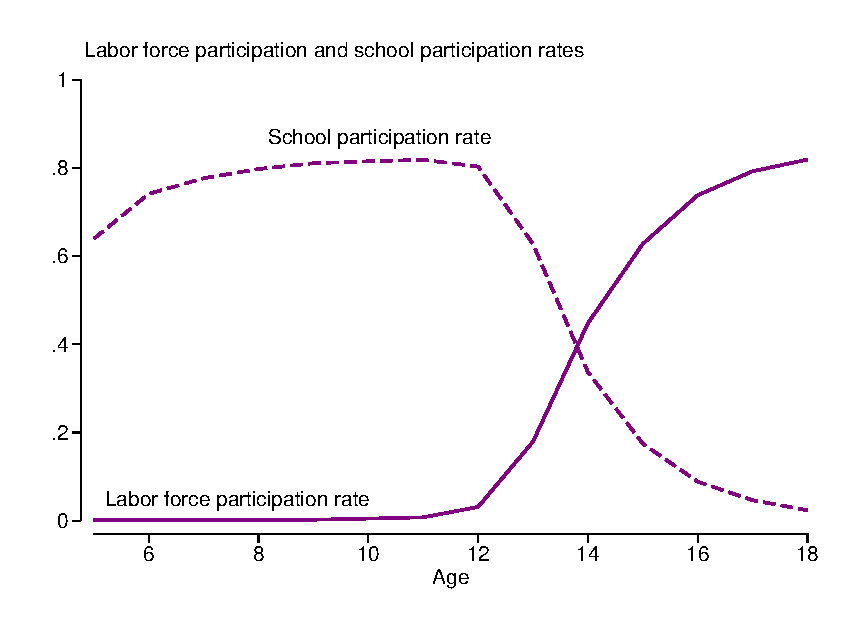
\includegraphics[width=1.0\textwidth]{../output/02_appendix/figure_a06.eps}
    \Fnote{This figure plots the labor force participation rate (solid line) and the rate of participation in schooling (dashed line) by age (5 to 18) in the 1881 Population Census of England, for male individuals residing in the County of London. An individual is considered to be in the labor force if any gainful occupation is reported in the census as measured by a valid Historical International Standard Classification of Occupations (HISCO) code. See Section~\ref{subsec:schooling-spec} for a description of how participation in schooling is coded. Results are similar in the 1891 census.}
    \label{fig:Fig_LFP_SchoolByAge}
\end{figure}

% Figure A7
\begin{figure}[!ht]
    \caption[Changes in father's occupation across adjacent censuses]{Changes in father's occupation across adjacent censuses}
    \centering
	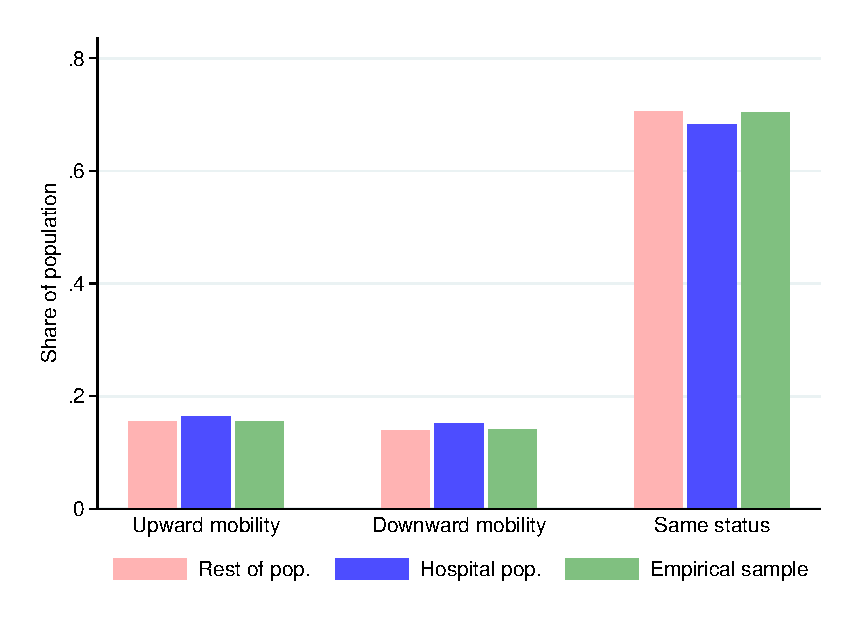
\includegraphics[width=1.0\linewidth]{../output/02_appendix/figure_a07.eps}
    \Fnote{This figure presents summary measures of occupational changes for fathers linked between the 1881 and 1891 or 1891 and 1901 censuses. It shows the share of fathers whose occupational rank increases (upward mobility), decreases (downward mobility) or stays the same (same status) from one census to the next. Shares are shown separately for the subset of the main empirical sample with linked fathers (green), the rest of the hospital population (blue), and the rest of the overall population (pink). See Online Appendix~\ref{sec:linking-fathers} for a description of the procedure for linking fathers.}
    \label{fig:intragen-fathers}
\end{figure}

% Figure A8
\begin{figure}[!ht]
\caption[Randomly assign lower father's SES to 15\% of patients 1000 times]{Randomly assign lower father's SES to 15\% of patients 1000 times}
\centering
\begin{subfigure}{0.49\textwidth}
	\centering
	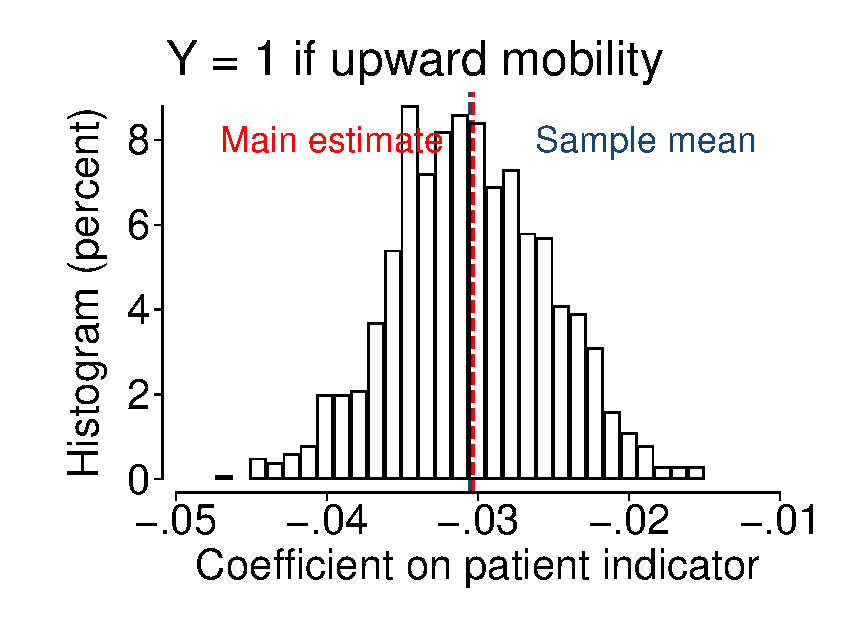
\includegraphics[width=1.00\linewidth]{../output/02_appendix/figure_a08_panel_01.eps}
\end{subfigure}
\begin{subfigure}{0.49\textwidth}
	\centering
	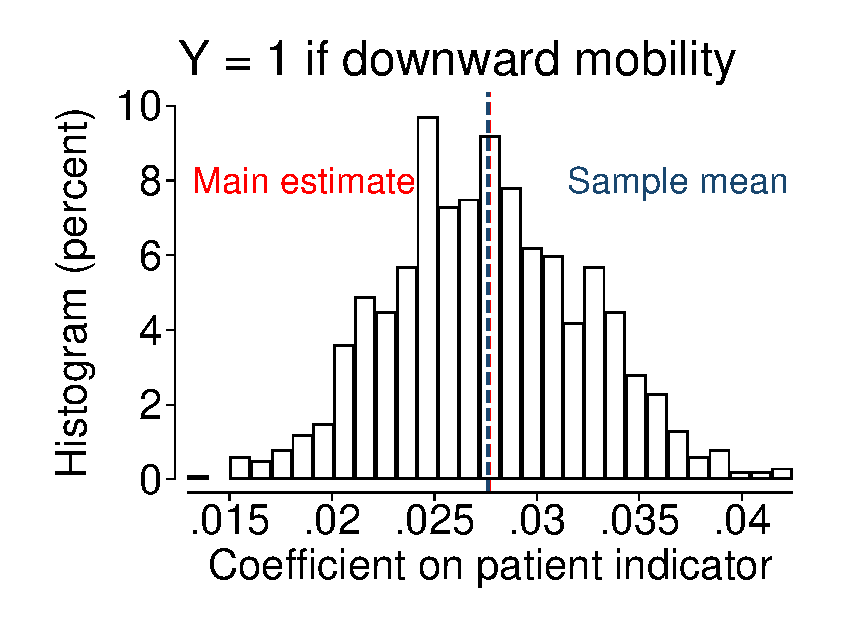
\includegraphics[width=1.00\linewidth]{../output/02_appendix/figure_a08_panel_02.eps}
\end{subfigure}
\begin{subfigure}{0.49\textwidth}
	\centering
	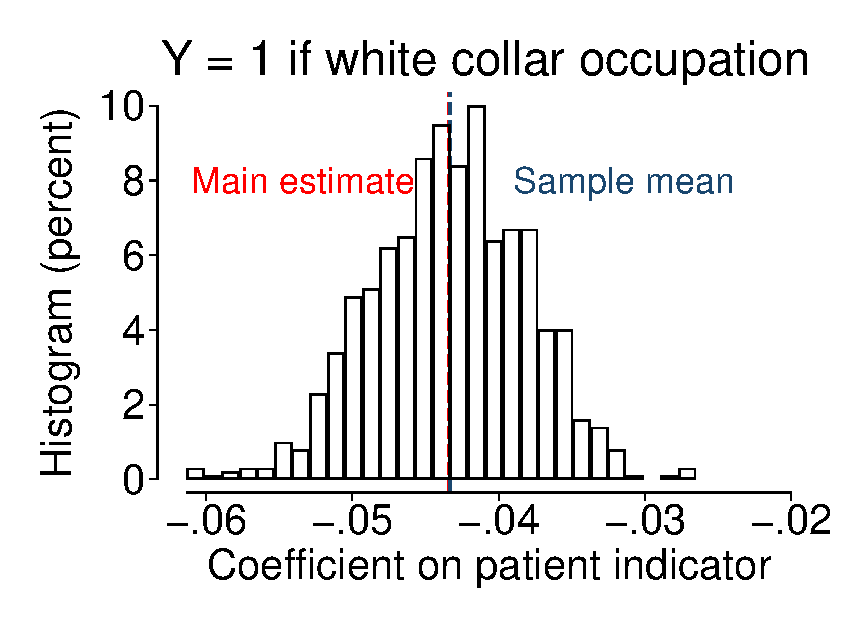
\includegraphics[width=1.00\linewidth]{../output/02_appendix/figure_a08_panel_03.eps}
\end{subfigure}
\begin{subfigure}{0.49\textwidth}
	\centering
	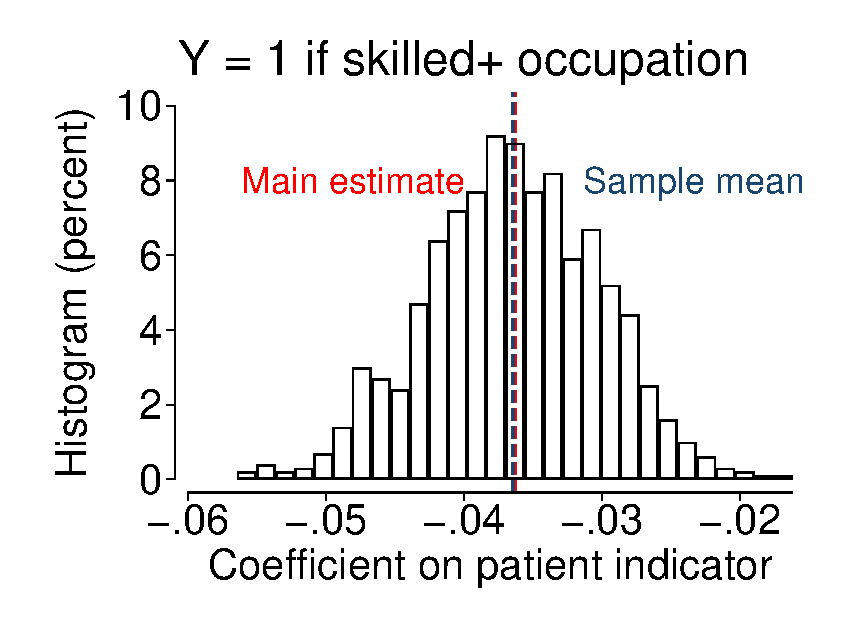
\includegraphics[width=1.00\linewidth]{../output/02_appendix/figure_a08_panel_04.eps}
\end{subfigure}
\begin{subfigure}{0.49\textwidth}
	\centering
	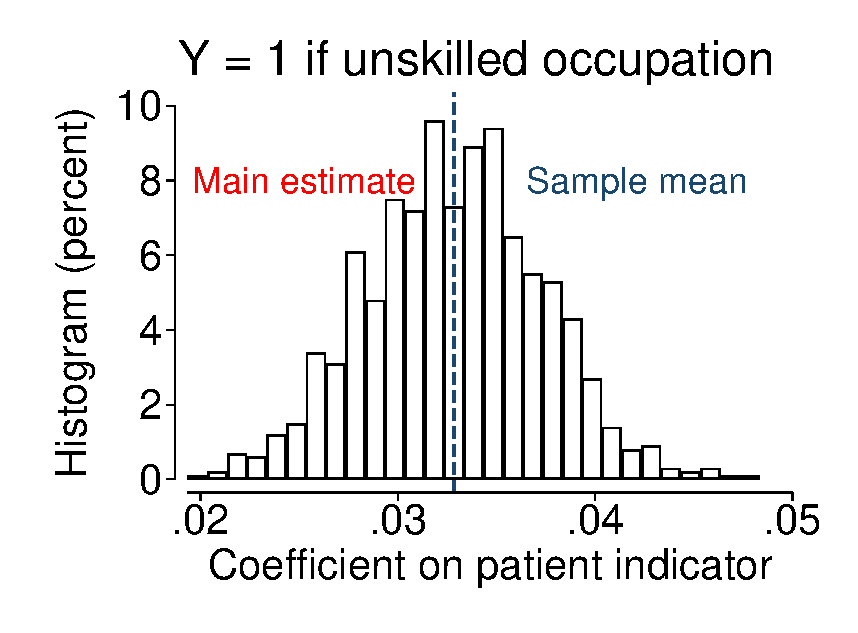
\includegraphics[width=1.00\linewidth]{../output/02_appendix/figure_a08_panel_05.eps}
\end{subfigure}
\begin{subfigure}{0.49\textwidth}
	\centering
	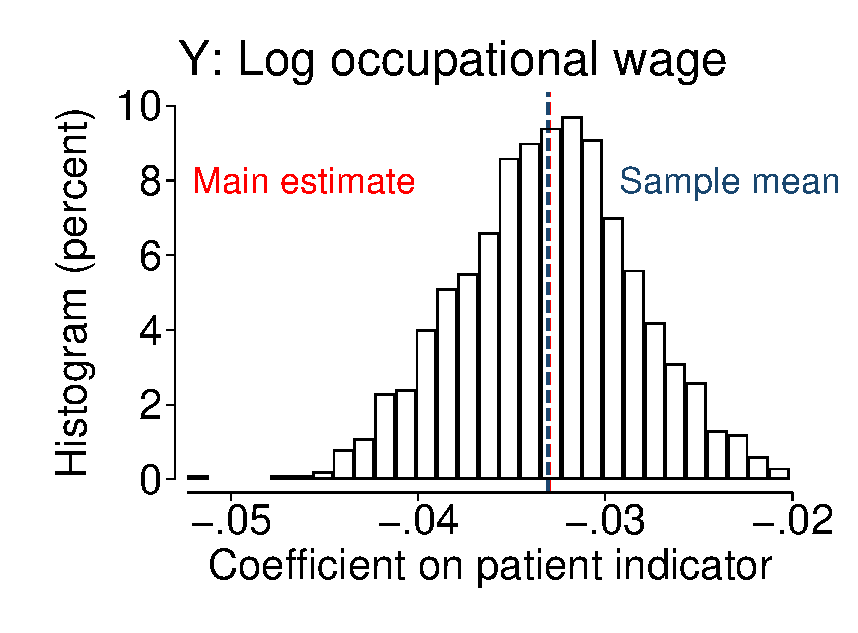
\includegraphics[width=1.00\linewidth]{../output/02_appendix/figure_a08_panel_06.eps}
\end{subfigure}
\Fnote{Each figure plots the distribution of estimated coefficients on the patient indicator from 1000 iterations of assigning the father's socioeconomic status (SES) to be one rank lower for 15 percent of the patients in the sample and re-estimating the main specification for the six dependent variables shown in Tables~\ref{tab:TabLR_Occup_Main}. When the father's SES is the lowest rank, it is assigned to be one rank higher for the non-hospitalized sibling only.}
\label{fig:randomize-sibs-father}
\end{figure}

% Figure A9
\begin{figure}[!ht]
\caption[Effects of hospitalization by common causes of admission]{Effects of hospitalization by common causes of admission}
\centering
\begin{subfigure}{0.325\textwidth}
	\centering
	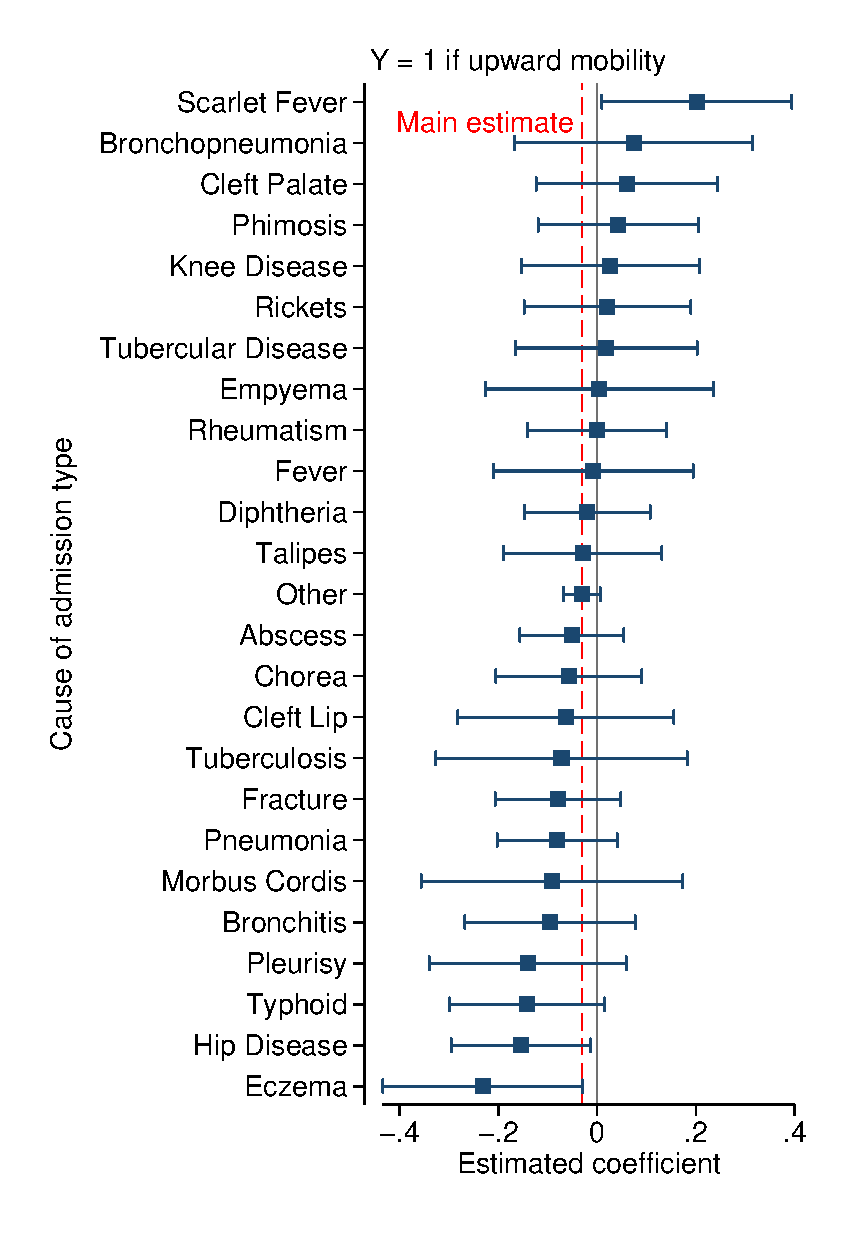
\includegraphics[width=1.00\linewidth]{../output/02_appendix/figure_a09_panel_1.eps}
\end{subfigure}
\begin{subfigure}{0.325\textwidth}
	\centering
	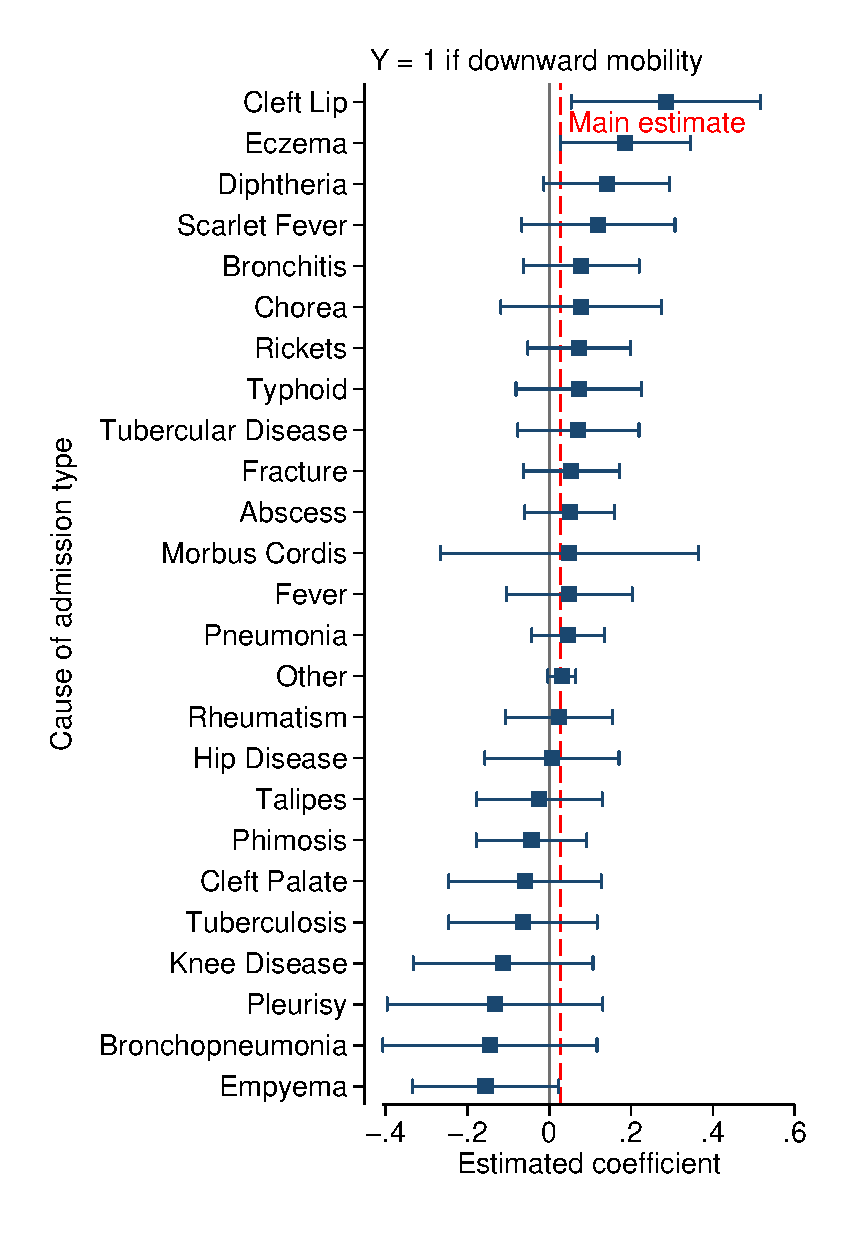
\includegraphics[width=1.00\linewidth]{../output/02_appendix/figure_a09_panel_2.eps}
\end{subfigure}
\begin{subfigure}{0.325\textwidth}
	\centering
	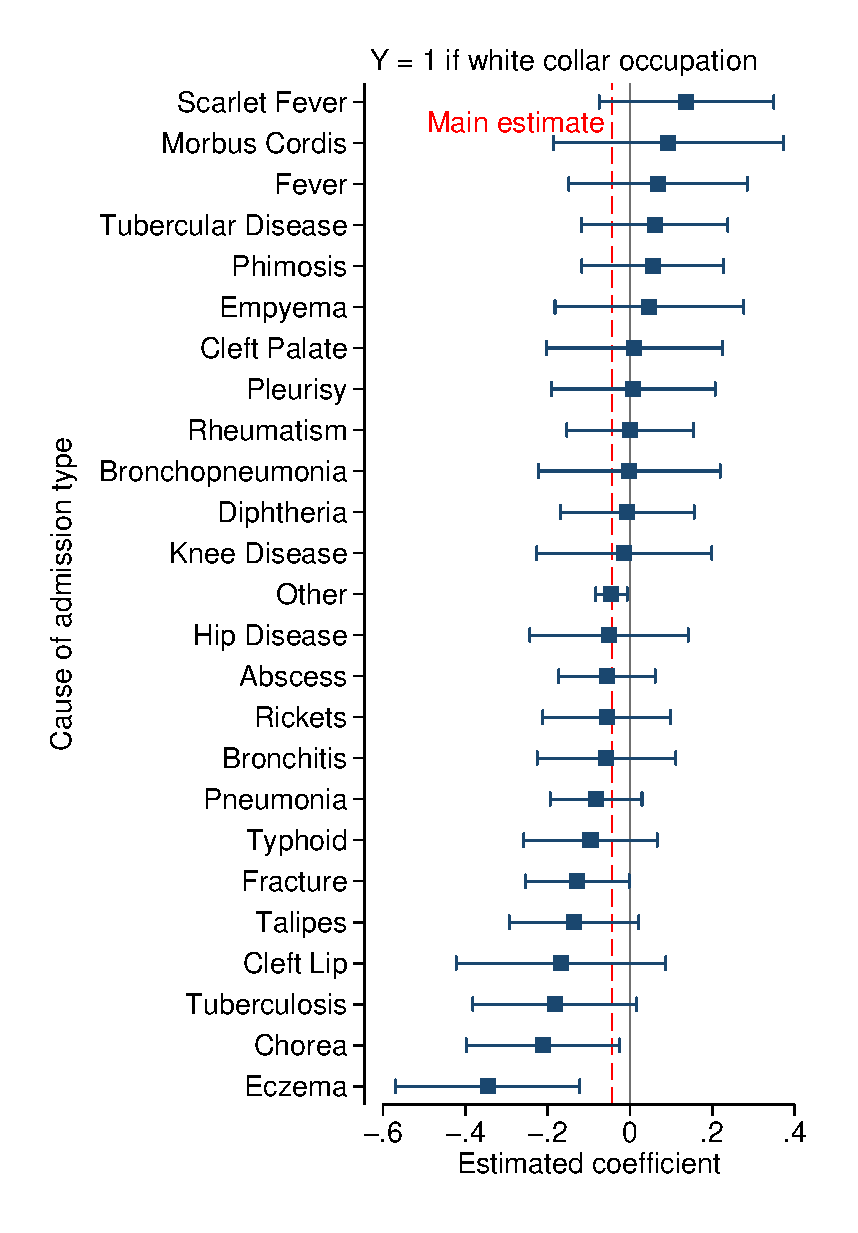
\includegraphics[width=1.00\linewidth]{../output/02_appendix/figure_a09_panel_3.eps}
\end{subfigure}
\begin{subfigure}{0.325\textwidth}
	\centering
	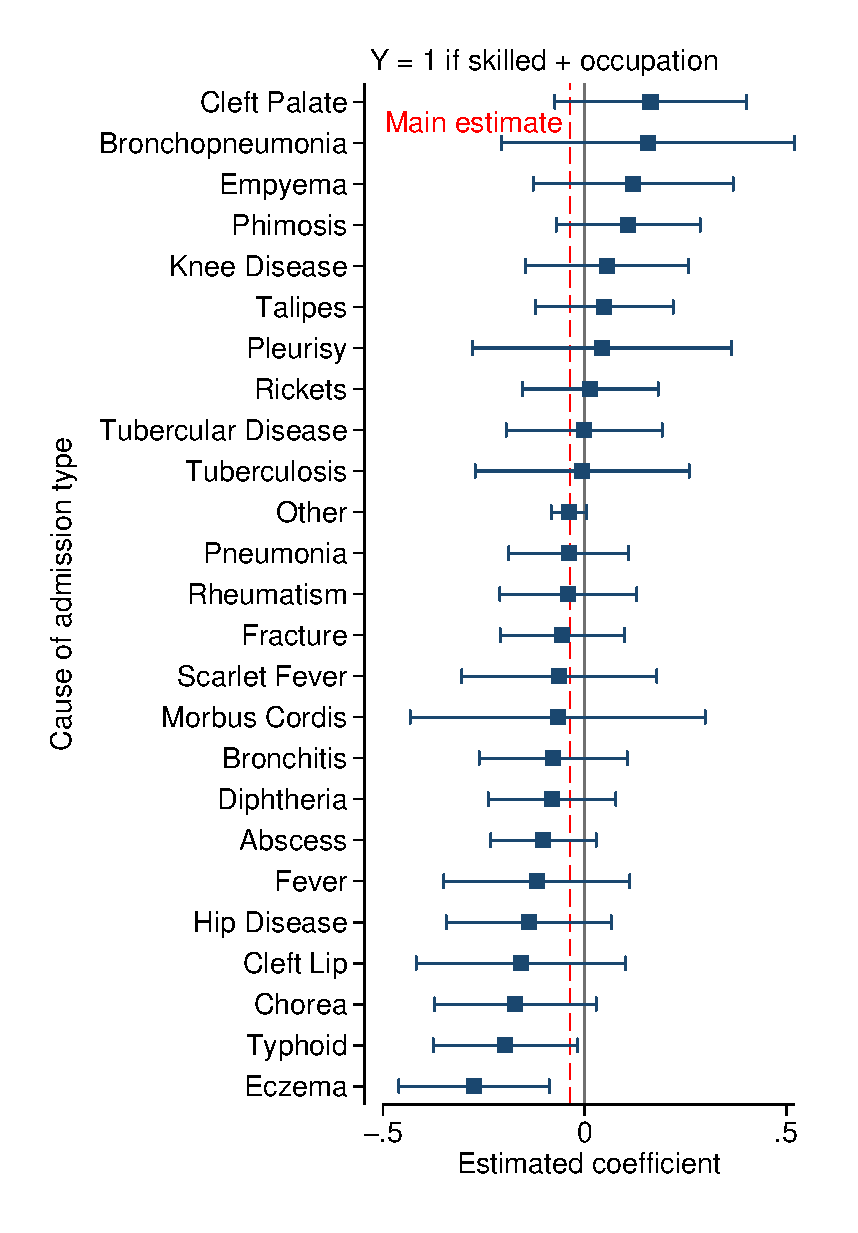
\includegraphics[width=1.00\linewidth]{../output/02_appendix/figure_a09_panel_4.eps}
\end{subfigure}
\begin{subfigure}{0.325\textwidth}
	\centering
	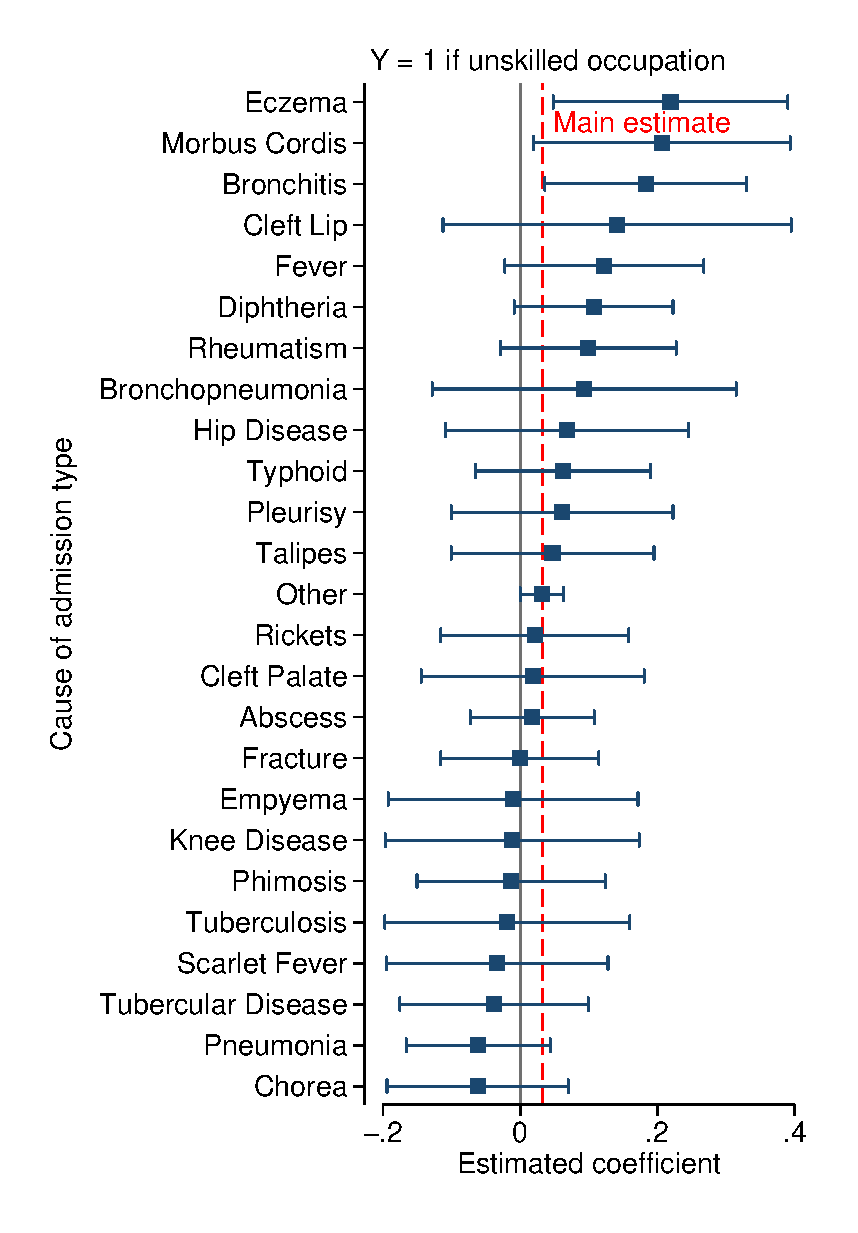
\includegraphics[width=1.00\linewidth]{../output/02_appendix/figure_a09_panel_5.eps}
\end{subfigure}
\begin{subfigure}{0.325\textwidth}
	\centering
	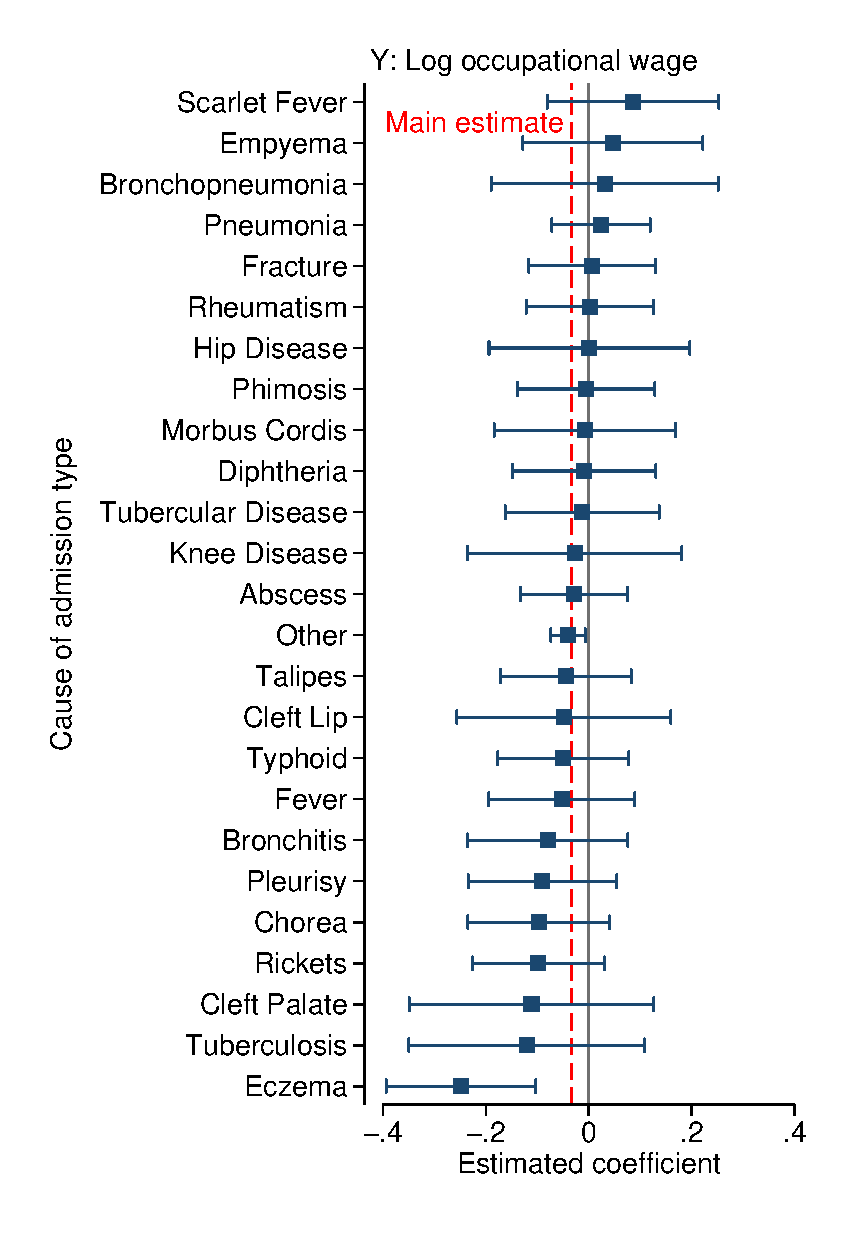
\includegraphics[width=1.00\linewidth]{../output/02_appendix/figure_a09_panel_6.eps}
\end{subfigure}
\Fnote{Each figure plots estimated coefficients on indicators for the most common causes of admission listed in Table~\ref{tab:top-25-coa}, and 95-percent confidence intervals from a single sibling fixed effects regression with one of six long-run occupational outcome variables shown in Table~\ref{tab:TabLR_Occup_Main}. In addition to the causes of admission plotted, the regressions include an indicator for admissions for multiple categories, as well as the same set of control variables listed in Table~\ref{tab:TabLR_Occup_Main}. Standard errors are clustered by childhood household.}
\label{fig:coa-common}
\end{figure}

% Figure A10
\begin{figure}[!ht]
\caption[Effects of hospitalization by hospital admission type]{Effects of hospitalization by hospital admission type}
\centering
\begin{subfigure}{0.49\textwidth}
	\centering
	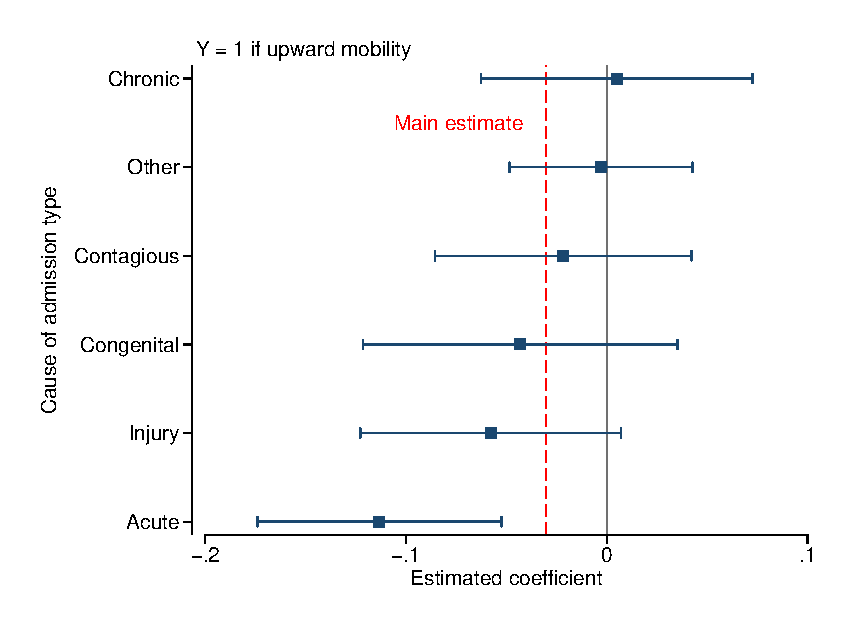
\includegraphics[width=1.00\linewidth]{../output/02_appendix/figure_a10_panel_1.eps}
\end{subfigure}
\begin{subfigure}{0.49\textwidth}
	\centering
	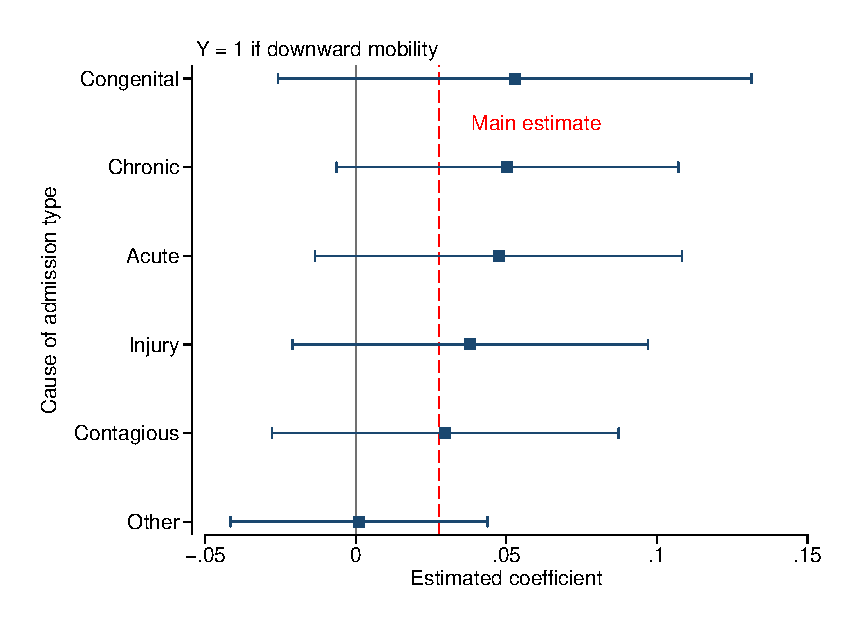
\includegraphics[width=1.00\linewidth]{../output/02_appendix/figure_a10_panel_2.eps}
\end{subfigure}
\begin{subfigure}{0.49\textwidth}
	\centering
	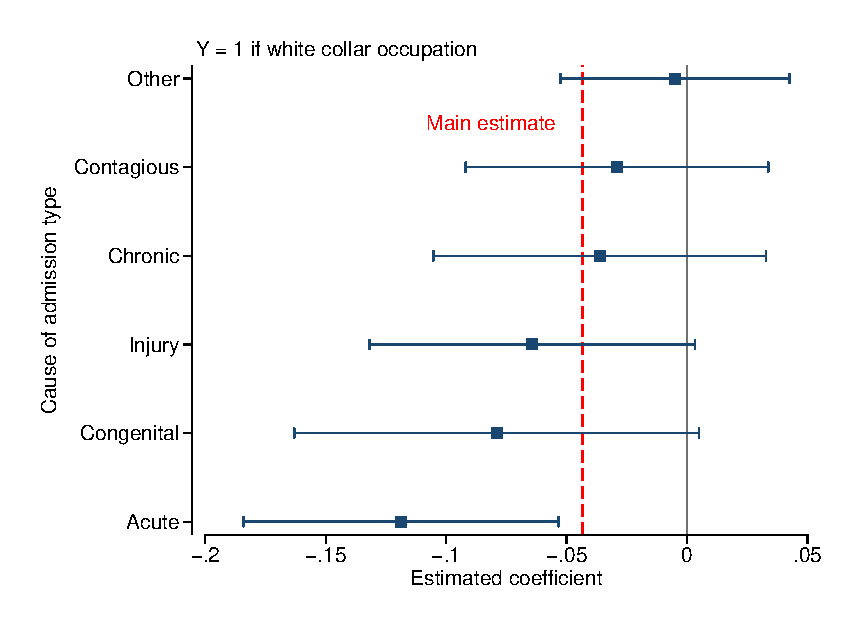
\includegraphics[width=1.00\linewidth]{../output/02_appendix/figure_a10_panel_3.eps}
\end{subfigure}
\begin{subfigure}{0.49\textwidth}
	\centering
	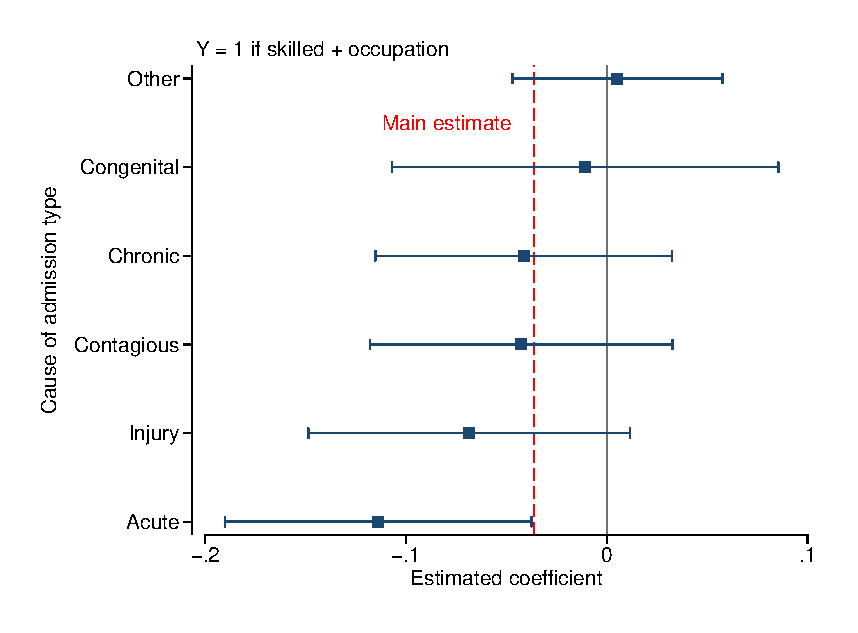
\includegraphics[width=1.00\linewidth]{../output/02_appendix/figure_a10_panel_4.eps}
\end{subfigure}
\begin{subfigure}{0.49\textwidth}
	\centering
	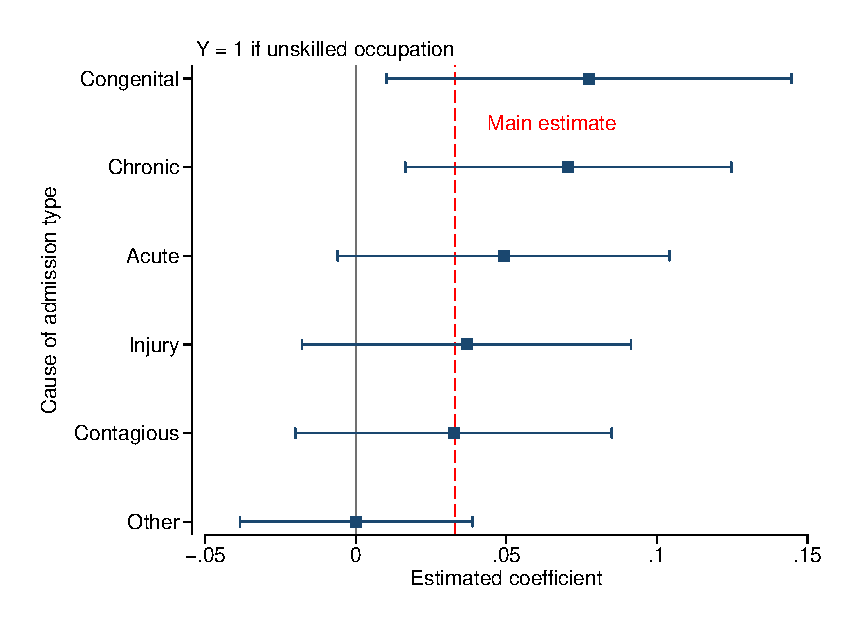
\includegraphics[width=1.00\linewidth]{../output/02_appendix/figure_a10_panel_5.eps}
\end{subfigure}
\begin{subfigure}{0.49\textwidth}
	\centering
	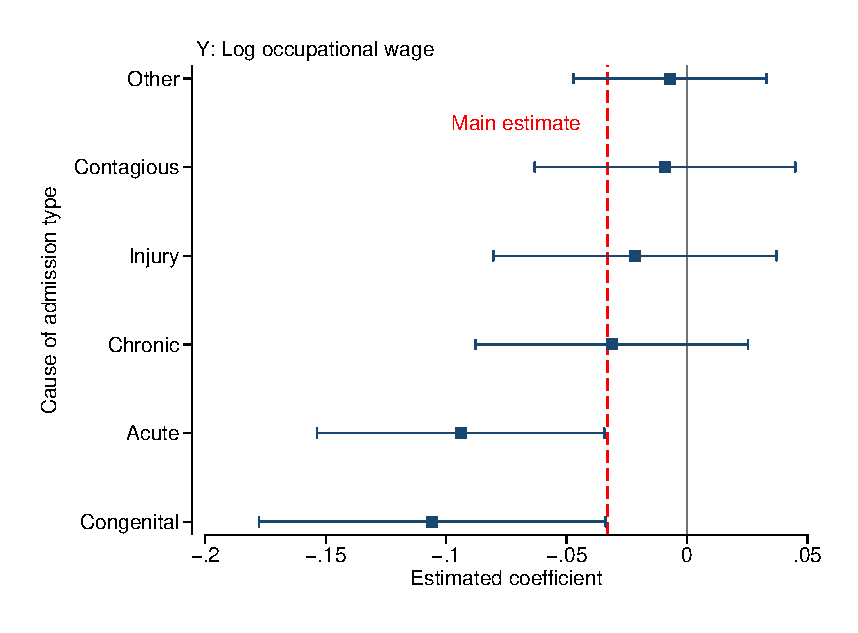
\includegraphics[width=1.00\linewidth]{../output/02_appendix/figure_a10_panel_6.eps}
\end{subfigure}
\Fnote{Each figure plots the estimated coefficients on indicators for a type of hospital admission and 95-percent confidence intervals from a single sibling fixed effects regression with one of six long-run occupational outcome variables shown in Table~\ref{tab:TabLR_Occup_Main}. In addition to the causes of admission plotted, the regressions include an indicator for admissions for multiple categories, as well as the same set of control variables listed in Table~\ref{tab:TabLR_Occup_Main}. Standard errors are clustered by childhood household.}
\label{fig:coa-type}
\end{figure}

% Figure A11
\begin{figure}[!ht]
\caption[Effects of hospitalization by body system classification]{Effects of hospitalization by body system classification}
\centering
\begin{subfigure}{0.49\textwidth}
	\centering
	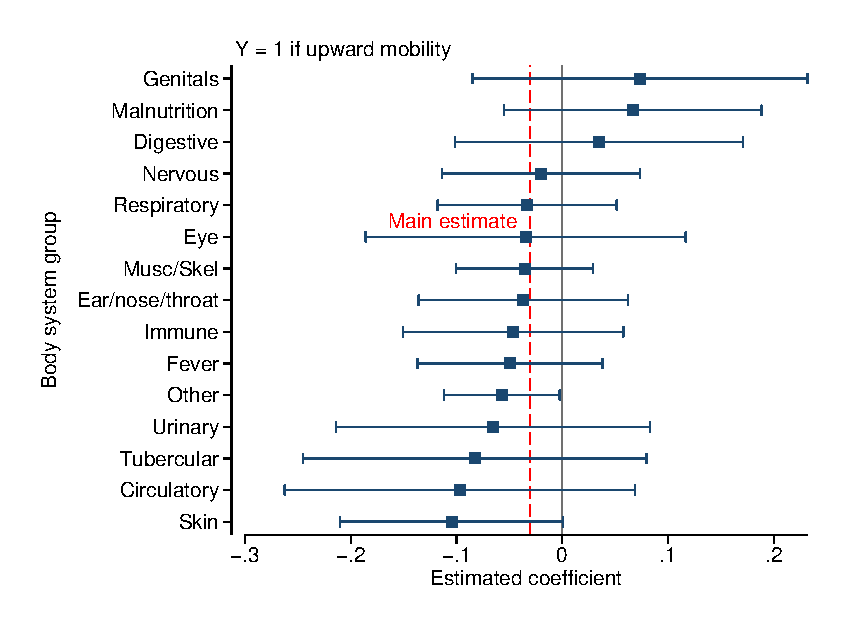
\includegraphics[width=1.00\linewidth]{../output/02_appendix/figure_a11_panel_1.eps}
\end{subfigure}
\begin{subfigure}{0.49\textwidth}
	\centering
	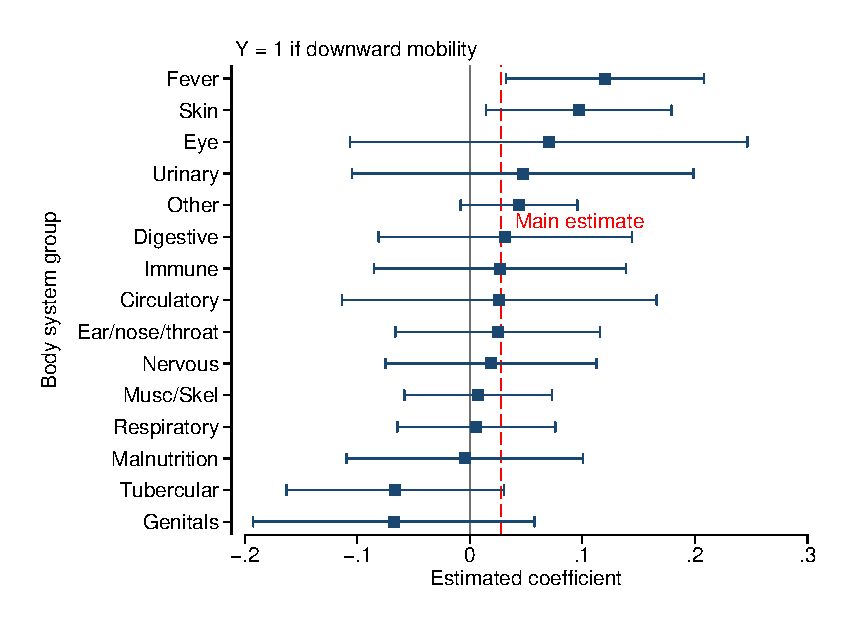
\includegraphics[width=1.00\linewidth]{../output/02_appendix/figure_a11_panel_2.eps}
\end{subfigure}
\begin{subfigure}{0.49\textwidth}
	\centering
	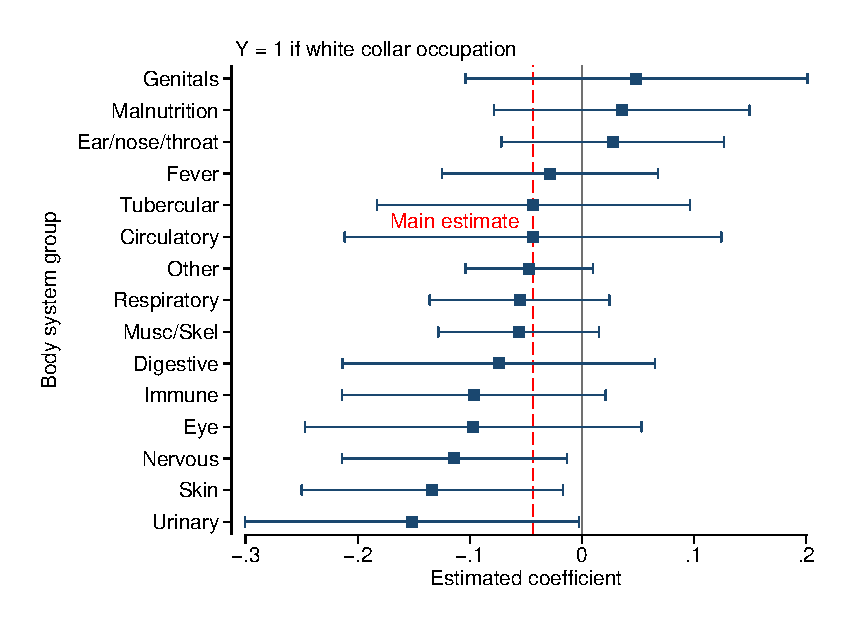
\includegraphics[width=1.00\linewidth]{../output/02_appendix/figure_a11_panel_3.eps}
\end{subfigure}
\begin{subfigure}{0.49\textwidth}
	\centering
	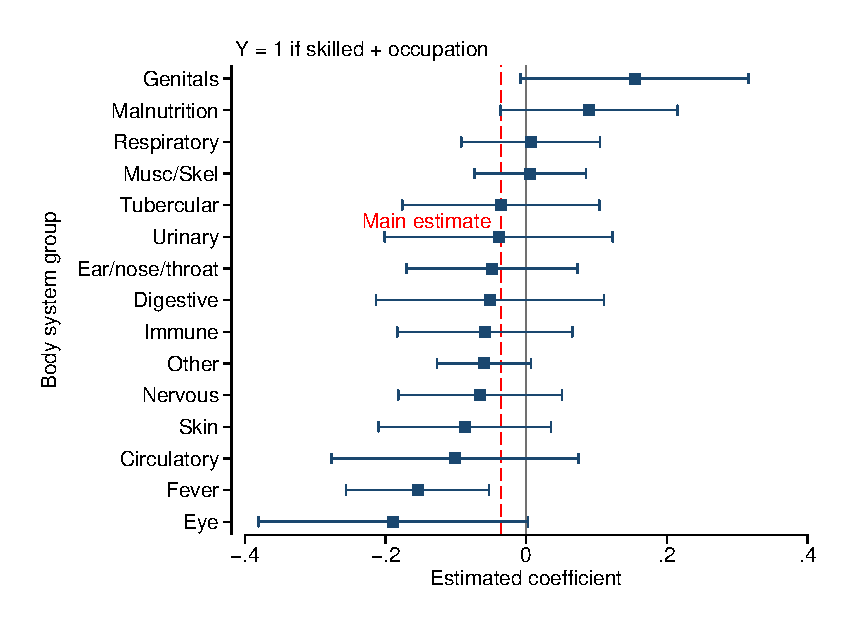
\includegraphics[width=1.00\linewidth]{../output/02_appendix/figure_a11_panel_4.eps}
\end{subfigure}
\begin{subfigure}{0.49\textwidth}
	\centering
	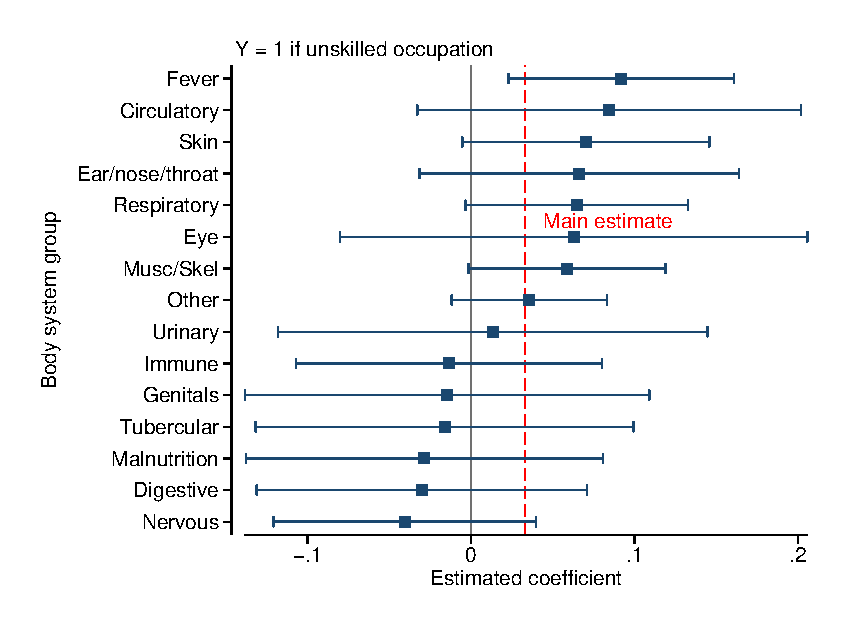
\includegraphics[width=1.00\linewidth]{../output/02_appendix/figure_a11_panel_5.eps}
\end{subfigure}
\begin{subfigure}{0.49\textwidth}
	\centering
	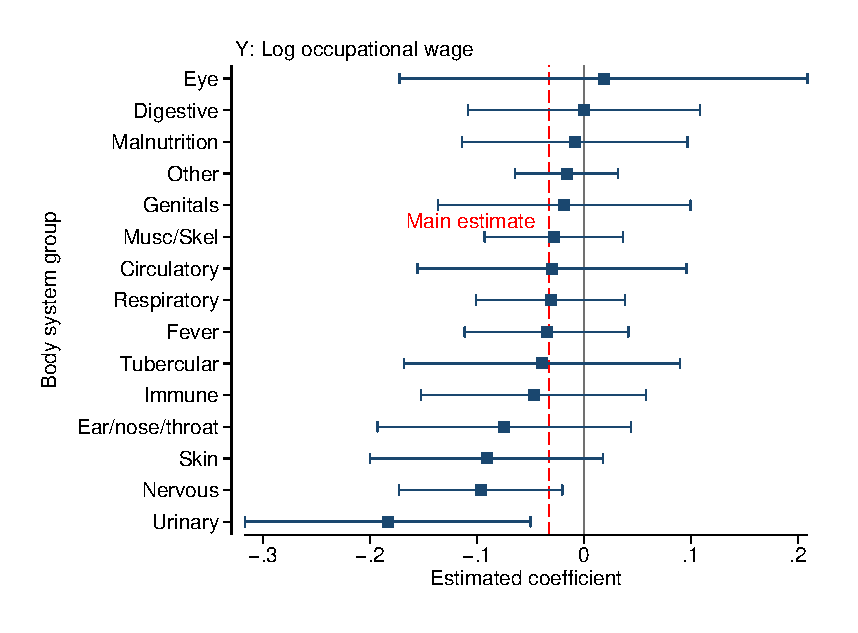
\includegraphics[width=1.00\linewidth]{../output/02_appendix/figure_a11_panel_6.eps}
\end{subfigure}
\Fnote{Each figure plots the estimated coefficients on indicators for the type of hospital admission, classified by body system, and 95-percent confidence intervals from a single sibling fixed effects regression with one of six long-run occupational outcome variables shown in Table~\ref{tab:TabLR_Occup_Main}. In addition to the causes of admission plotted, the regressions include an indicator for admissions for multiple categories, as well as the same set of control variables listed in Table~\ref{tab:TabLR_Occup_Main}. Standard errors are clustered by childhood household.}
\label{fig:coa-bodypt}
\end{figure}

% Figure A12
\begin{figure}[!ht]
\caption[Randomly assign treatment (=1) to 10\% of siblings 1000 times]{Randomly assign treatment (=1) to 10\% of siblings 1000 times}
\centering
\begin{subfigure}{0.49\textwidth}
	\centering
	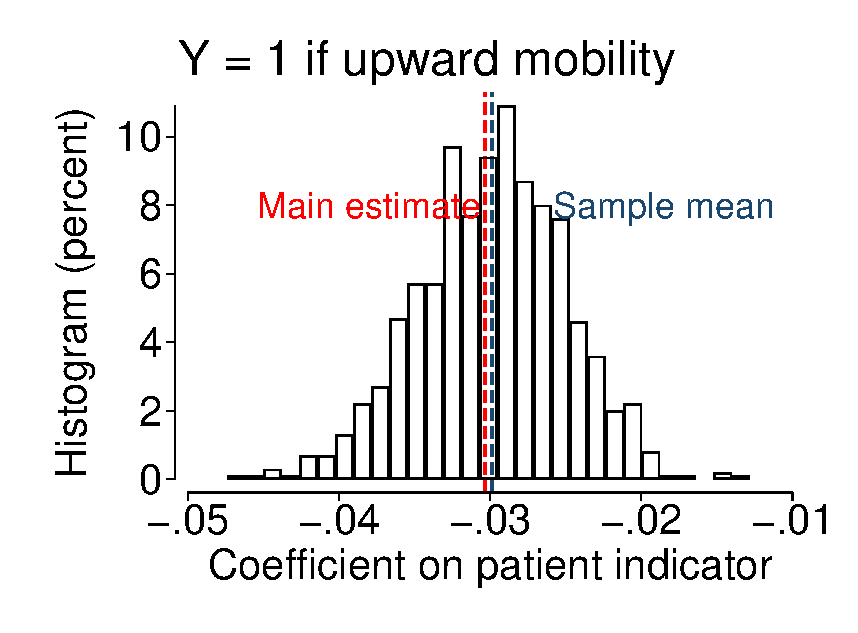
\includegraphics[width=1.00\linewidth]{../output/02_appendix/figure_a12_panel_01.eps}
\end{subfigure}
\begin{subfigure}{0.49\textwidth}
	\centering
	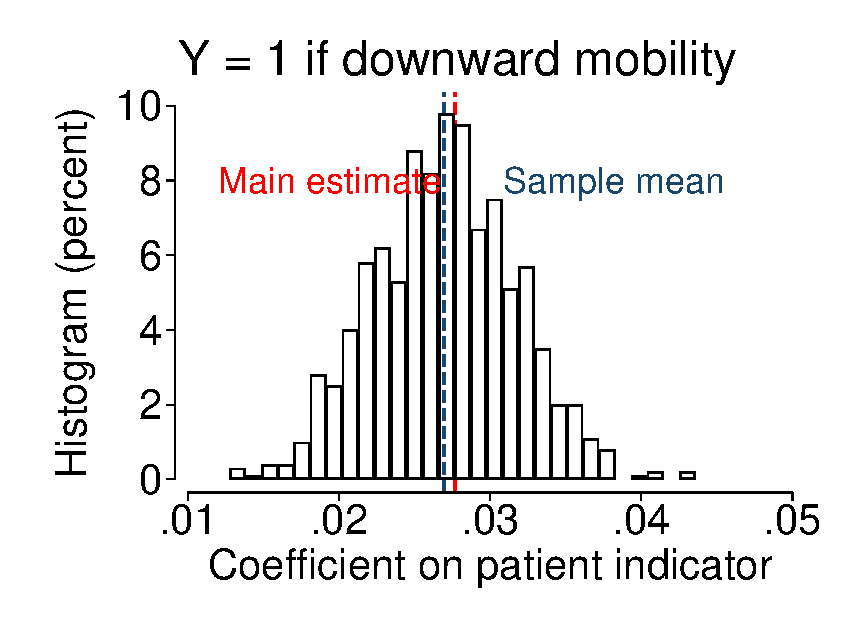
\includegraphics[width=1.00\linewidth]{../output/02_appendix/figure_a12_panel_02.eps}
\end{subfigure}
\begin{subfigure}{0.49\textwidth}
	\centering
	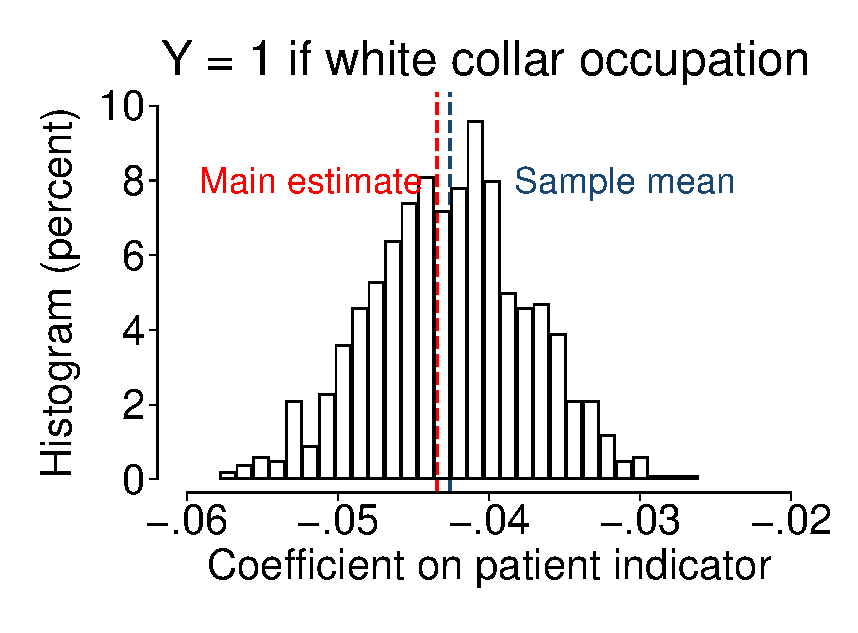
\includegraphics[width=1.00\linewidth]{../output/02_appendix/figure_a12_panel_03.eps}
\end{subfigure}
\begin{subfigure}{0.49\textwidth}
	\centering
	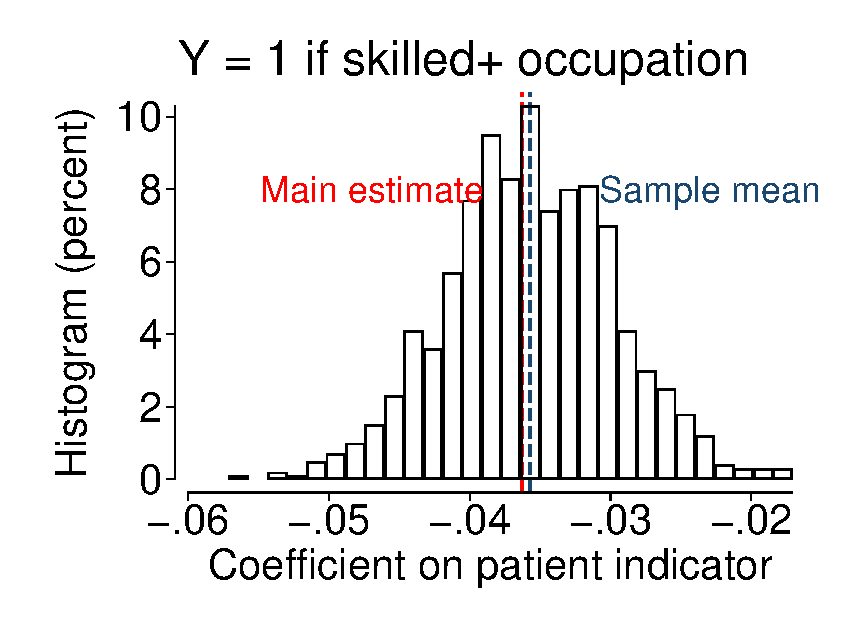
\includegraphics[width=1.00\linewidth]{../output/02_appendix/figure_a12_panel_04.eps}
\end{subfigure}
\begin{subfigure}{0.49\textwidth}
	\centering
	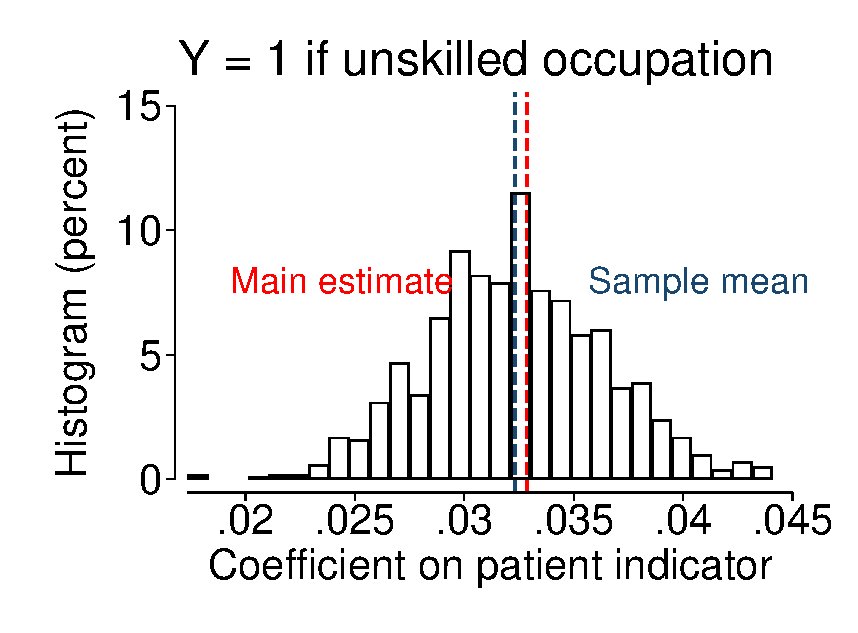
\includegraphics[width=1.00\linewidth]{../output/02_appendix/figure_a12_panel_05.eps}
\end{subfigure}
\begin{subfigure}{0.49\textwidth}
	\centering
	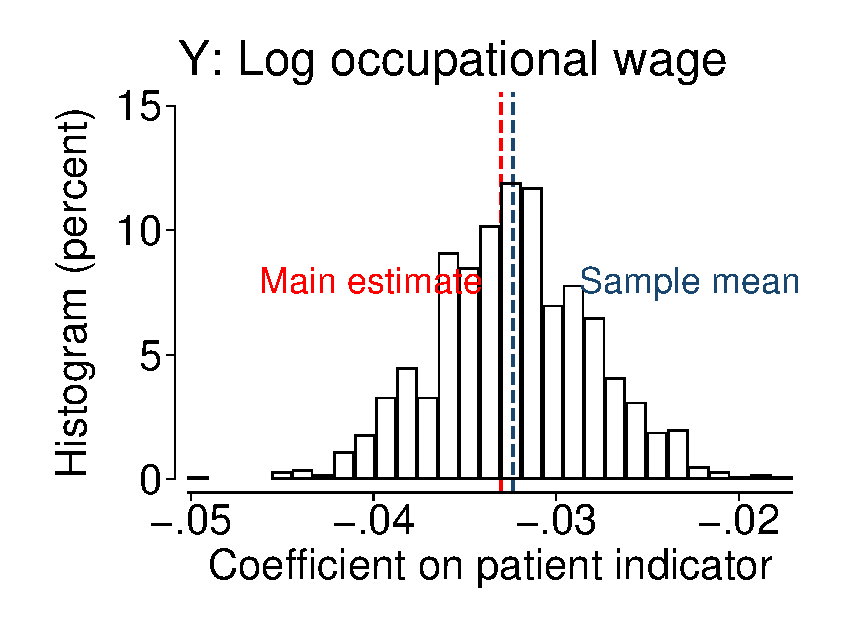
\includegraphics[width=1.00\linewidth]{../output/02_appendix/figure_a12_panel_06.eps}
\end{subfigure}
\Fnote{Each figure plots the distribution of estimated coefficients on the hospitalization indicator from 1,000 iterations of assigning the treatment indicator equal to one for 10 percent of the non-hospitalized siblings in the sample and re-estimating the main specification for the six dependent variables shown in Table~\ref{tab:TabLR_Occup_Main}.}
\label{fig:randomize-sibs}
\end{figure}

% Figure A13
\begin{figure}[!ht]
  \caption[Density of health deficiency index in population vs. estimation sample]{Density of health deficiency index in population vs. estimation sample}
    \centering
    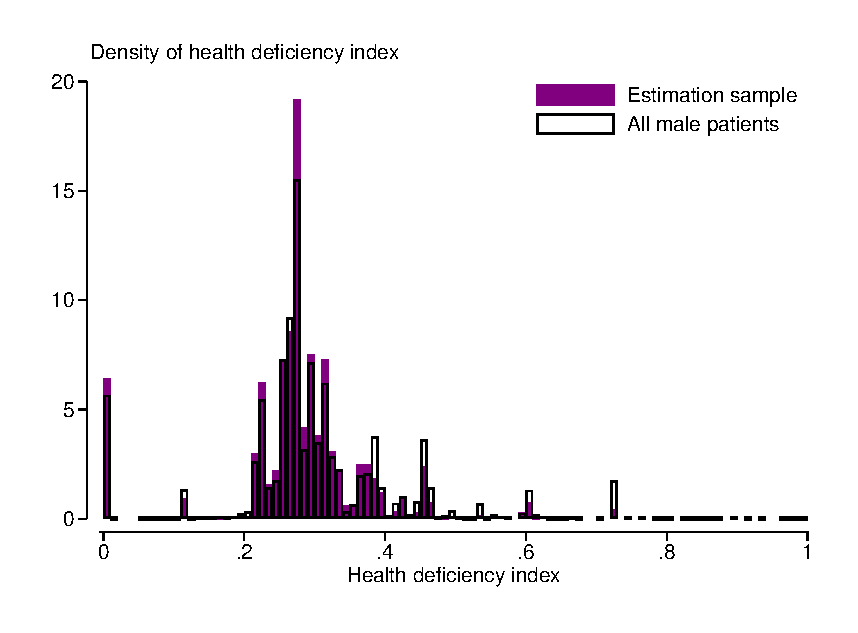
\includegraphics[width=\linewidth]{../output/02_appendix/figure_a13.eps}
    \Fnote{This figure presents a histogram of the health deficiency index for the population of male patients admitted to the hospitals in the full sample (white) and for the patients in the final estimation sample (solid purple). See Online Appendix~\ref{sec:health-deficiency-index} for a description of the procedure used to construct the health deficiency index.}
  \label{fig:hi-density}
\end{figure}

% Figure A14
\begin{figure}[!ht]
\caption[Robustness of effects on single marital status]{Robustness of effects on likelihood of being enumerated as a single adult}
\centering
\begin{subfigure}{0.66\textwidth}
    \centering
    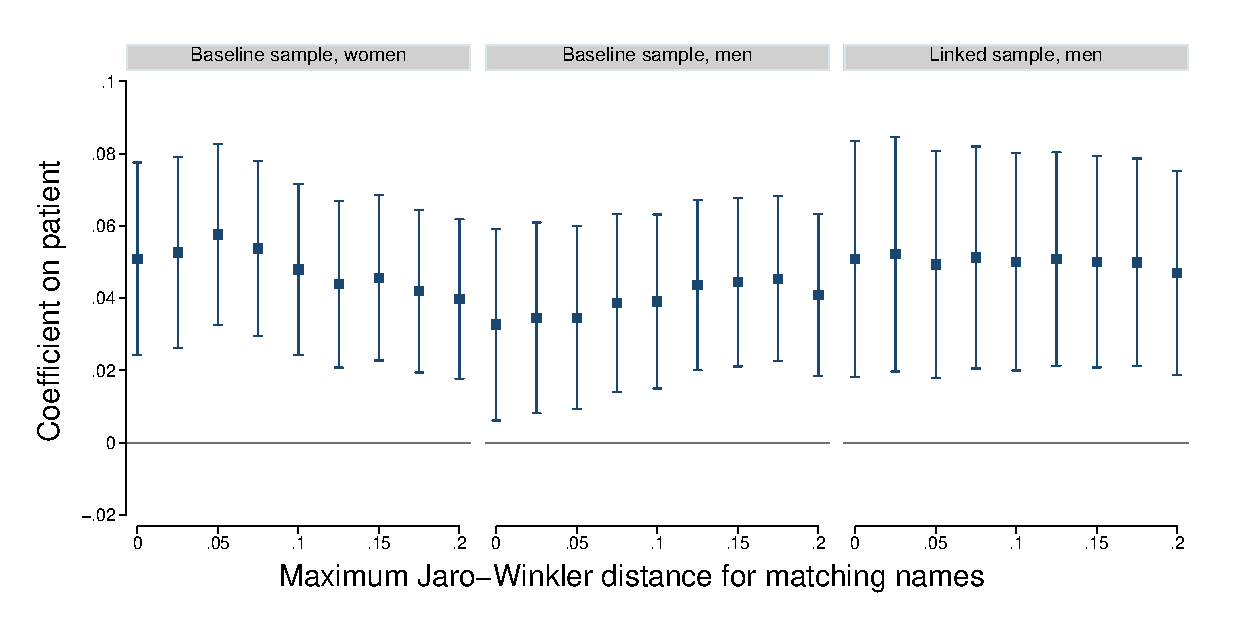
\includegraphics[width=1.0\linewidth]{../output/02_appendix/figure_a14_panel_1.eps}
    \caption{Changing Jaro-Winkler distance threshold}
    \label{fig:jw-robust-single}
\end{subfigure}
\begin{subfigure}{0.66\textwidth}
    \centering
    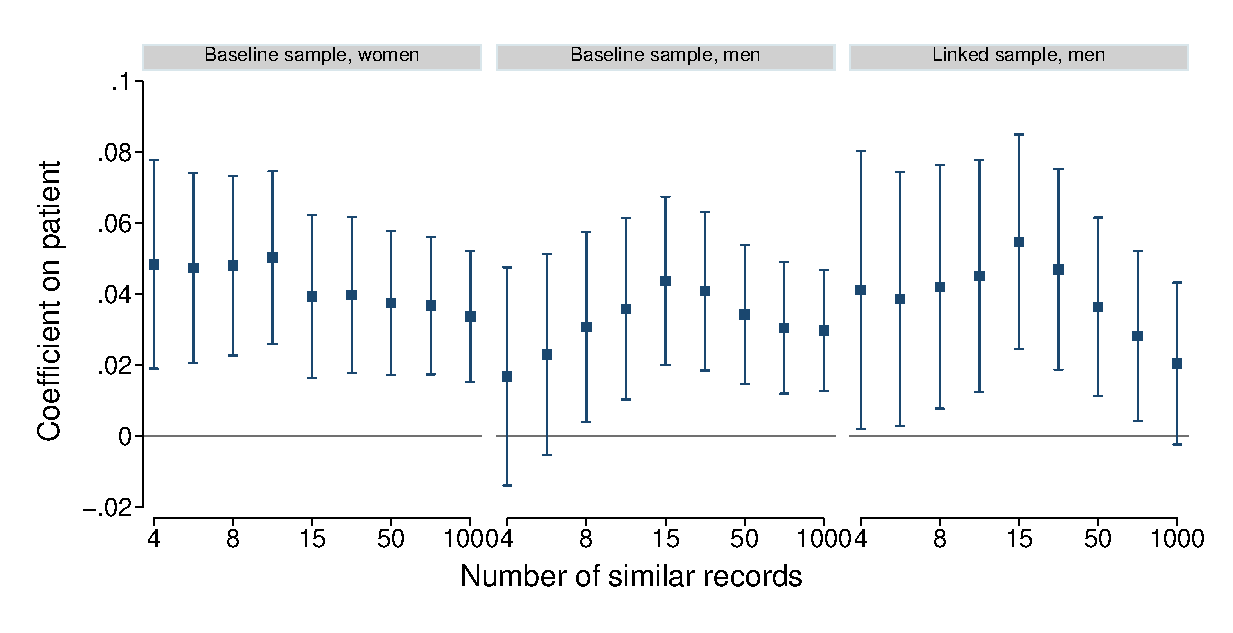
\includegraphics[width=1.0\linewidth]{../output/02_appendix/figure_a14_panel_2.eps}
    \caption{Changing similar names threshold}
    \label{fig:sim-records-robust-single}
\end{subfigure}
\begin{subfigure}{0.66\textwidth}
    \centering
    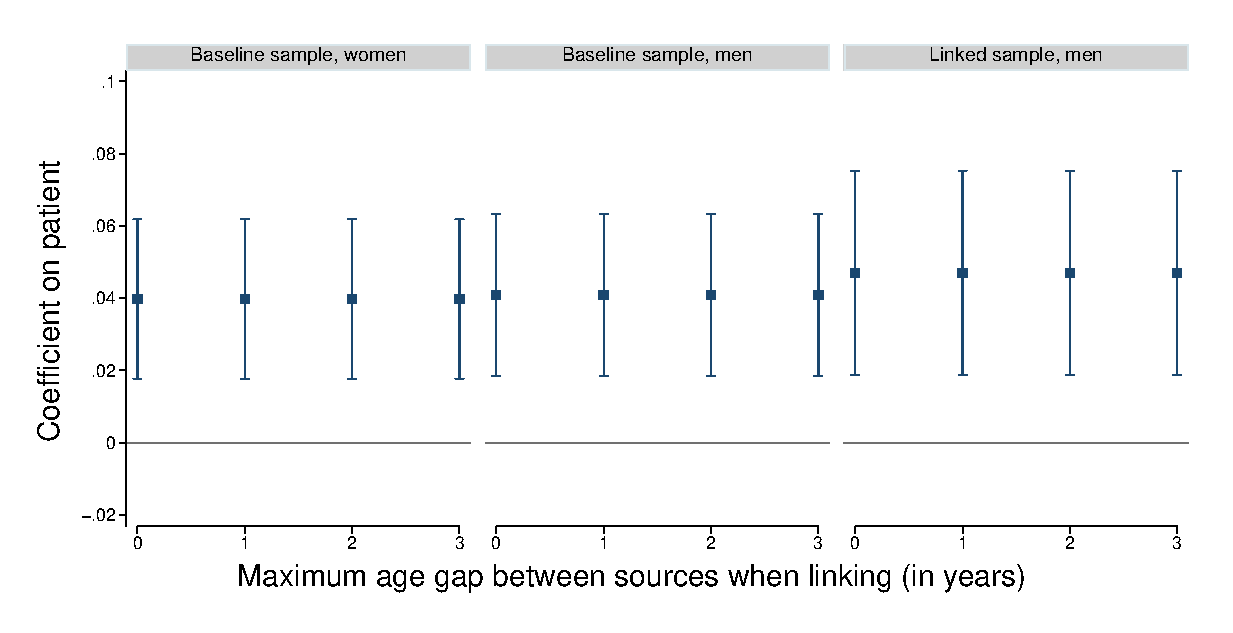
\includegraphics[width=1.0\linewidth]{../output/02_appendix/figure_a14_panel_3.eps}
    \caption{Changing age-gap threshold for linking}
    \label{fig:age-dist-robust-single}
\end{subfigure}
\Fnote{This figure presents estimated coefficients on the patient indicator variable and 95-percent confidence intervals from robustness specifications for the effects on the likelihood of being enumerated as a single adult. See Table~\ref{tab:TabLR_Single_Marital_Status} for a description of the empirical specifications and Figures~\ref{fig:jw-robust} to \ref{fig:age-gap-robust} for a description of the robustness exercises.}
\label{fig:robust-single-marital-status}
\end{figure}

% Figure A15
\begin{figure}[!ht]
    \caption{Share of population ever married by age and sex in 1911}    
    \centering
    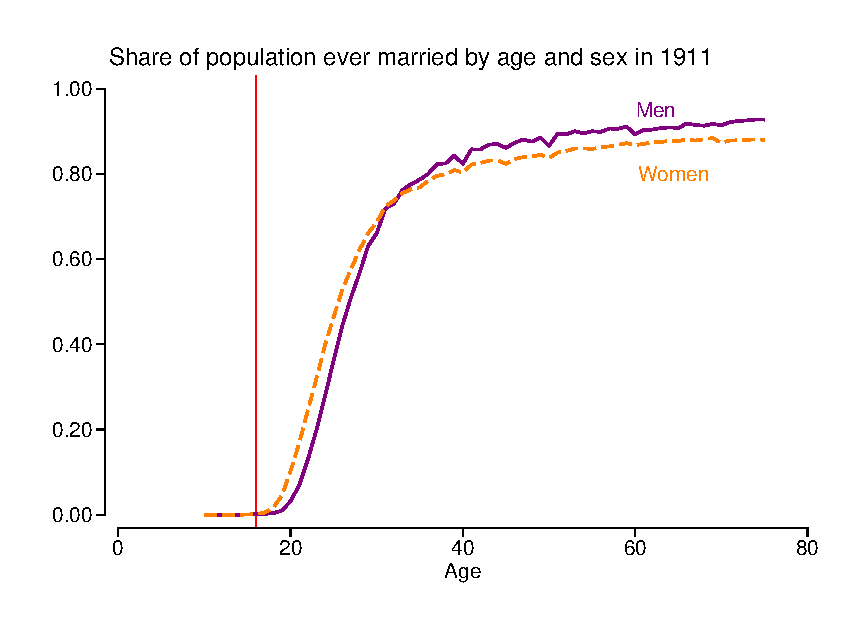
\includegraphics[width=1.0\textwidth]{../output/02_appendix/figure_a15.eps}
    \Fnote{This figure plots the share of the population of England enumerated in the 1911 census who report ever being married by age, starting at age 15. Separate plots are shown by gender for men (solid purple line) and women (dashed orange line). Ever married consists of the following codes in response to the question on marital status: married with spouse present in household, married without spouse present, divorced, or widowed. The excluded group consists of individuals who report single marital status. Individuals with missing age, gender, or marital status are excluded from the analysis. The vertical red line indicates age 16 to highlight the  restriction that individuals must be no older than age 15 when enumerated in the childhood census in the analysis of marital status. }
    \label{fig:Fig_MarriedByAge}
\end{figure}

\end{document}